\documentclass[12pt]{article}
\usepackage[OT4]{fontenc}
\usepackage[polish]{babel}
\usepackage[legalpaper, margin=2cm]{geometry}
\usepackage{mathtools}
\usepackage{float}
\usepackage{hyperref}
\usepackage{svg}
\usepackage{graphicx}
\usepackage{placeins}
\usepackage{chngcntr}

\newif\ifpokazsekcjaszesc
\pokazsekcjaszesctrue
% \pokazsekcjaszesctrue

\newcommand{\wykrespngwniosek}[4]{%
\begin{figure}[H]
    \centering
    \ifpokazsekcjaszesc
        \includegraphics[width=0.72\textwidth,height=0.24\textheight,keepaspectratio]{#1}%
    \else
        \fbox{%
            \parbox[c][0.20\textheight][c]{0.72\textwidth}{%
                \centering
                \texttt{#1}\\[0.4em]
                \small miejsce na wykres
            }%
        }%
    \fi
    \caption{#2}
    \label{fig:#3}
\end{figure}
\noindent\textbf{Wniosek:} #4
\par\vspace{0.2cm}
}


\title{Sprawozdanie z pierwszej połowy projektu\\
Przedmiotu "Wizualizacja Danych"}
\author{Grupa Pon 14:15 - 17:00, \\zespół 4 - Jan Domański, Maciej Kurzydłowski, Jan Machowski}
\date{sem. 26L}

\begin{document}
\maketitle
\tableofcontents
\newpage

% Proponowana struktura rozdziału
% 1. Źródło danych
% 2. Opis zbioru i istotnych pojęć - o czym jest, pojęcia z nim związane, kolumny, czy dane są kateg / liczb/
% 3. Wizualizacja + krótki opis co pokazuje
% 4. Wnioski


% \subsubsection{}
% \begin{figure}[H]
%     \includegraphics[width=\textwidth]{phts/}
%     \caption{}
% \end{figure}


\section{Standarized price-to-income ratio (MATLAB)}

Przygotowane przez: Jan Machowski

\subsection{Źródło danych}
\href{https://ec.europa.eu/eurostat/databrowser/view/tipsho60/default/table?lang=en}{Eurostat tipsho60 - Standarized price-to-income ratio - annual data}\\
\url{https://ec.europa.eu/eurostat/databrowser/view/tipsho60/default/table?lang=en}

\subsection{Opis zbioru i istotnych pojęć}
\begin{itemize}
    \item Zbiór przedstawia uśrednione wartości PTI dla poszczególnych krajów;
    \item Dane zostały zebrane na przestrzeni lat 2000 - 2024;
    \item Dane pochodzą z 27 krajów członkowskich Unii Europejskiej;
    \item \textbf{AGDI} - Average Gross Domestic Income - skorygowany dochód do dyspozycji brutto gospodarstwa domowego;
    \item \textbf{PTI} - Price-to-income, ustandaryzowany stosunek średniej ceny mieszkania do AGDI gospodarstwa domowego;
    \item \textbf{RoC} - Rate of Change, współczynnik zmiany wartości PTI wzgledem poprzedniego roku (w roku 2000 wartości NaN);
    \item \textbf{Większość danych z okresu 2000 - 2004 są estymatami} - należy brać te dane na poprawkę;
    \item Zwiększenie / zmniejszenie indeksu PTI nie oznacza jednoznacznie zwiększenia / zmniejszenia ceny mieszkania 
    - oznacza że \textbf{stosunek mieszkania wzgledem zarobku się zmienił};
    \item Indeks PTI dla kraju można interpretować jako \textbf{średnią, względną wartość domu w danym kraju}.
\end{itemize}


\subsection{Wizualizacje zbioru}
\subsubsection{Statystyka opisowa Price-to-Income}
\begin{figure}[H]
    \includesvg[width=\textwidth]{phts/1/svg/1.1}
    \caption{Statystyka opisowa danych PTI względem kraju.}
\end{figure}

Wykres przedstawia podstawowe statystyki opisowe wartości PTI względem średniej długoterminowej dla zbioru krajów. 
Średnia na przestrzeni lat prezentuje się równomiernie, wszystkie kraje znajdują się w zakresie 90\% - 120\% PTI.
Widać jednak, że odchylenie jednego z państw - Rumunii - dominuje nad pozostałymi. Sugeruje to, że dane dla tego 
kraju będą bardzo zmienne, co również widać po wartościach miniumalnej i maksymalnej Rumunii.


\subsubsection{Indeks Price-to-Income względem kraju}
\begin{figure}[H]
    \includesvg[width=\textwidth]{phts/1/svg/1.2}
    \caption{Wartość indeksu PTI względem kraju na przestrzeni lat względem roku 2015.}
\end{figure}

Jak wspomniano w opisie, dane przedstawione na wykresie są PTI wzgledem roku 2015 w poszczególnym kraju - stąd kumulacja linii w tym punkcie.
Dla klarowności, dane podzielono na Europę Wschodnią i Europę Zachodnią. Najbardziej zmienna jest faktycznie Rumunia, uzyskująca szczyt w 2007 roku 
powyżej 250\% PTI, i stopniowo spadająca od tego momentu.

Na wykresie widać tendencję spadkową indeksów PTI wszystkich krajów na przestrzeni lat 2007 - 2015. Jest to w znacznym stopniu spowodowane
kryzysem na rynku mieszkaniowym z 2008 roku, zapoczątkowanym w Stanach Zjednoczonych. Jak widać, kryzys nie udeżył krajów Europy tak mocno, 
jak Stany Zjednoczone, ale wpływ globalnej gospodarki pod koniec lat 10 XXI wieku jest nie do podważenia.

\subsubsection{Price-to-Income w 2024 względem średniej długoterminowej}
\begin{figure}[H]
    \includesvg[width=\textwidth]{phts/1/svg/1.4}
    \caption{Indeks PTI krajów w 2024 roku względem średniej długoterminowej.}
\end{figure}

Wyrkes ten w intuicyjny sposób przedstawia różnicę najnowszej wartości indeksu PTI krajów Europejskich względem średniej długoterminowej.
Jak widać, najbardziej wartościowe domy Europejskie można znaleźć w Portugalii, Luksemburgu i Austrii. Warto zauważyć, że podział na Europę Wschodnią 
oraz Zachodnią nie determinuje tego czy mieszkania są średnio bardziej wartościowe niż w przeciwnej połowie podziału - zarówno w krajach "powyżej 0" 
oraz "poniżej 0" występują kraje wschodnie i zachodnie.  

\subsubsection{Zmiana Price-to-Income między 2000 a 2024}
\begin{figure}[H]
    \includesvg[width=\textwidth]{phts/1/svg/1.7}
    \caption{Zmiana indeksu PTI krajów między 2000 a 2024 rokiem.}
\end{figure}

Dzięki powyższej wizualizacji jesteśmy w stanie klarownie określić, czy od roku 2000 (lub pierwszego dostępnego w zbiorze) do roku 2024 (lub ostatniego) 
średnia wartość mieszkania wzrosła, czy zmalała. Podobnie jak w przypadku poprzedniego wykresu, widzimy podział względnie równy, gdzie najbardziej odstającymi
krajami są Luksemburg (na plus - wartość wzrosła) oraz Bułgaria (na minus - wartość zmalała).

\subsubsection{Zmiana Price-to-Income między minimum a maksimum}
\begin{figure}[H]
    \includesvg[width=\textwidth]{phts/1/svg/1.8}
    \caption{Zmiana indeksu PTI krajów między najmniejszą a największą dostępną wartością.}
\end{figure}

Na tym wykresie również dominuje Luksemburg, dwukrotnie przewyżając następny w kolejności kraj - Szwecję. Oczywiście nie oznacza to że Luksemburg ma 
średnio najbardziej wartościowe mieszkania, tylko że odczuł największą całkowitą różnicę wartości od 2000 do 2024 roku.

\subsubsection{Statystyki opisowe Rate of Change}
\begin{figure}[H]
    \includesvg[width=\textwidth]{phts/1/svg/1.6}
    \caption{Statystyki opisowe wartości indeksu RoC.}
\end{figure}

RoC jest indeksem, który wskazuje zmianę PTI względem poprzedniego roku. Niedziwnym jest więc, że większość wartości RoC mieści się w przedziale od -10 pp.
do +10 pp. - aż 90\% wszystkich zmian zamyka się w tym przedziale. Jak wynika ze średniej i mediany, statystycznie jest nieznacznie więcej dodatnich RoC 
niż ujemnych - średnia RoC wynosi 0.5pp. a mediana 0.3pp. 

Analizujący wykres po prawej stronie, nie trudno zauważyć że w każdym przedziale poza 2007-2012 doświadczono nieujemnych średnich wartości RoC. 
Oczywiście, większa ujemność wartości z lat 2007-2012 spowodowana jest wyżej wspomnianym kryzysem mieszkanowym. 


\subsubsection{Indeks Rate of Change względm kraju}
\begin{figure}[H]
    \includesvg[width=\textwidth]{phts/1/svg/1.3}
    \caption{Wartość indeksu RoC względem kraju na przestrzeni lat.}
    \label{wykres:1_8}
\end{figure}

Analizując wykres pokazujący RoC z podziałem na Europę Wschodnią i Zachodnią jesteśmy w stanie stwierdzić, że RoC jest wartością bardziej chaotyczną niż 
PTI. Natomiast, analogicznie do poprzedniego wykresu, Rumunia przoduje wartościami maksymalnymi RoC a, o dziwo, w roku szczytowym dorównuje jej Polska.

\subsubsection{Heatmap wartości Rate of Change}
\begin{figure}[H]
    \includesvg[width=\textwidth]{phts/1/svg/1.5}
    \caption{Heatmap'a wartości Rate of Change krajów na przestrzeni lat.}
\end{figure}

Na wykresie typu heatmap klarownie widać jak kraje na przestrzeni lat zmagały się ze zmianami indeksu PTI. Widzimy, że rok 2005 i 2006 miały szczytowe wartości pozytywnych 
dla niektórych państw (Bułgaria, Litwa, Łotwa, Luksemburg), który niechybnie upadły w w latach 2008-2010. Po tym, mieszanka różnych kolorów odzwierciedla sytuację na 
Rysunku \ref{wykres:1_8} - chaotyczne ruchy zarówno w kierunku pozytywnym jak i negatywnym.

\subsubsection{Wyrkesy dla Polski}
\begin{figure}[H]
    \includesvg[width=\textwidth]{phts/1/svg/1.10}
    \caption{Wykresy PRI, RoC na przestrzeni lat dla Polski.}
\end{figure}

Skupiając się wyłącznie na polsce, widać tendencyjny spadek w latach 2008 - 2012 obecny dla pozostałych krajów Europy. Ciekawym jednak jest fakt, iż do aż 2017 roku
RoC było negatywne - oznacza to, że wartości mieszkań statystycznie malały w porównaniu z latami poprzednimi, a dopiero w 2018 roku zaczęły rosnąć i utrzymały swój 
wzrost w czasach pandemicznych. Odzwierciedla to również PTI, które "odbija się" w roku 2017 i średnio idzie w górę od tamtego roku, z wyjątkiem 2022 i 2023 
gdzie wartość znacznie spada, prawdopodobnie z uwagi na wartość inflacji w okresie Pandemii.

\newpage
\subsection{Wnioski}
\begin{enumerate}
    \item Na przełomie lat 2008-2015, w większości krajów Europy indeks PTI drastycznie spadł, po czym powoli wzrastał;
    \item 85\% wartości Rate of Change na przestrzeni wszystkich lat znajduje się w przedziale <-10 pp; 10pp>. Sugeruje to, że gospodarka mieszkaniowa jest, średnio, stabilna.
    \item Specjalnym przypadkiem jest Rumunia, w której PTI i RoC są bardzo zmienne i odstające od pozostałych krajów.
\end{enumerate}


\newpage
\section{Noclegi i miejsca do spania dla turystów w Europie (MATLAB)}

Przygotowane przez: Jan Machowski

\subsection{Źródło danych}
\href{https://ec.europa.eu/eurostat/databrowser/view/tour_cap_nuts2dc__custom_12660565/default/table}
{Eurostat\ tour\_cap\_nuts2dc - Establishments and Bed-places in Tourist Accommodation by Urbanisation \& Coastal type} \\
\url{https://ec.europa.eu/eurostat/databrowser/view/tour_cap_nuts2dc__custom_12660565/default/table}

\subsection{Opis zbioru i istotnych pojęć}
\begin{itemize}
    \item Dane zostały zbierane na przestrzeni lat 2012 - 2024;
    \item Dane pochodzą z 27 krajów członkowskich Unii Europejskiej;
    \item Granulacja danych występuje względem państw, województw (NUTS2), miast/przedmieść/wsi, miejsc przybrzeżnych/nieprzybrzeżnych;
    \item Dane dla niektórych krajów, zwłaszcza we wczesnych latach, są estymatami.
    \item \textbf{Placówka noclegowa / turystyczna} - ośrodek, który przyjmuje i kwateruje turystów z możliwością snu. 
            Wchodzą w to hotele, hostele, pola kempingowe i rekreacyjne, domki turystyczne i inne;
    \item \textbf{Miejsce do spania} - pełnoprawne, odpowiednie miejsce do odpoczynku nocnego dla jednej osoby.
            Wchodzą w to m.in. łóżko, rozkładana kanapa. Nie wchodzą w to m.in. nierozkładany fotel.
\end{itemize}


\subsection{Wizualizacje zbioru}

\subsubsection{Kraje z największą liczbą placówek noclegowych}
\begin{figure}[H]
    \includesvg[width=\textwidth]{phts/2/svg/2.1}
    \caption{20 państw Europy z największą liczbą placówek noclegowych w 2024 roku.}
\end{figure}
Na powyższym wykresie pokazane są kraje z największą liczbą placówek noclegowych w najnowszym dostępnym roku - 2024.
Jak widać, znaczną dominację sprawują Włochy mające ok. 265 000 zarejestrowanych placówek turystycznych na terenie państwa.
Jest to dwukrotnie więcej niż drugie w kolejności państwo - Chorwacja. Nie oznacza to jednak, że Włochy są w stanie
przenocować największą liczbę osób. Czy tak faktycznie jest zobaczymy na następnych wykresach.


\subsubsection{Kraje z największą liczbą miejsc do spania}
\begin{figure}[H]
    \includesvg[width=\textwidth]{phts/2/svg/2.2}
    \caption{20 państw Europy z największą liczbą miejsc do spania w 2024 roku.}
\end{figure}
Podobnie jak na poprzednim wykresie, Włochy zajęły pierwsze miejsce w liczbie miejsc do spania w całym kraju.
Zaskakująca sytuacja wydarzyła się na kolejnych miejscach - Chorwacja, która była druga względem liczby placówek turystycznych,
spadła na 7 miejsce. Pokazuje to oczywisty, ale istotny fakt: \textbf{nie każda placówka turystyczna ma taką samą liczbę 
miejsc do spania.} Jak widać, w Chorwacji jest wiele placówek które mają niedużą liczbę miejsc do spania, 
a przykładowo we Francji jest sytuacja odwrotna - mniej placówek, ale wysoka liczba miejsc do spania (np. hotele).


\subsubsection{Średnia liczba miejsc do spania na placówkę turystyczną}
Zależność przedstawioną w ramach opisach wyższego wykresu przedstawia następujący wykres:
\begin{figure}[H]
    \includesvg[width=\textwidth]{phts/2/svg/2.7}
    \caption{Średnia liczba miejsc do spania na placówkę turystyczną.}
\end{figure}
Niespodziewanym wynikiem jest Szwecja, która wyszła na czoło rankingu w perspektywie stosunku miejsc do spania 
do liczb placówek turystycznych. Sugeruje to jedno - Szwecja ma relatywnie mało placówek noclegowych, które mają relatywnie 
dużo miejsc do spania - hotele, hostele i tym podobne.
Włochy, kraj dotychczas dominujący, znajduje się na 16 miejscu. Można z tego wysnuć oczywisty wniosek: 
we Włoszech jest wiele małych placówek, które akceptują niewielką liczbę osób na noc.

Ciekawym jest fakt, że "przełęcz" między krajami dominującymi na dwóch poprzednich wykresach, a aktualnym, jest znacznie 
zmniejszona - wartości odstające są dominujące tylko i wyłącznie w specyficznych perspektywach. 
Dodatkowo, patrząc na pozostałe kraje w rankingu, klarownie widać iż kształt figury stworzonej przez ich słupki jest
analogiczny na wspomnianych trzech wykresach. Potwierdza to wcześniej nawiązaną hipotezę. 


\subsubsection{Zmienność liczby placówek noclegowych na przestrzeni lat}
\begin{figure}[H]
    \includesvg[width=\textwidth]{phts/2/svg/2.3}
    \caption{Wyrkes zmienności liczby placówek noclegowych na przestrzeni lat.}
\end{figure}
Z uwagi na dominację dwóch państw Europy w perspektywie liczby placówek noclegowych, tj. Włoch i Chorwacji, 
pozostałe kraje wyglądają jakby miały relatywnie stałą liczbę placówek. Jest to zła koncepcja - zmiany działy się, 
i były względnie znaczące dla danych krajów, jednak są przykryte skalą państw dominujących. Poniższy wykres przedstawia 
te zależności bez obecności Włoch i Chorwacji:
\begin{figure}[H]
    \includesvg[width=\textwidth]{phts/2/svg/2.11}
    \caption{Wyrkes zmienności liczby placówek noclegowych na przestrzeni lat - bez Włoch i Chorwacji.}
\end{figure}
Jak widać, zmiany nie wyglądają tak samo nieznacznie jak na wykresie z dominującymi państwami. Przykładowo, 
liczba hoteli stopniowo spada w Niemczech, rośnie w Hiszpanii a w Grecji miała znaczny spadek na początku pandemii Koronawirusa.
Warto zauważyć, że nawet po pozbyciu się Włoch i Chorwacji, skala dobrze ilustrująca pozostałe państwa to $ 10^4 $ . 
Ponownie biorąc Grecję, oznacza to zamknięcie ok. 16000 placówek turystycznych tylko i wyłącznie między 2019 a 2020 rokiem. 

\subsubsection{Indeks wzrostu liczby placówek turystycznych na przestrzeni lat}
\begin{figure}[H]
    \includesvg[width=\textwidth]{phts/2/svg/2.4}
    \caption{Wykres zmienności indeksu wzrostu liczby placówek turystycznych na przestrzeni lat.}
\end{figure}
Jesteśmy w stanie spojrzeć na całkowity wzrost liczby placówek z perspektywy indeksu względem jednej wyznaczonej daty, 
w celu porównania względnego wzrostu możliwości przyjęcia turystów w wybranych krajach Europy. Biorąc początkowe dane jako 
dane z roku 2012 i obliczając owy indeks widać, że mimo ogromnej liczby hoteli we Włoszech ich względny wzrost nie był aż tak duży, jak w przypadku Chorwacji oraz, 
co zaskakujące, Hiszpanii - kraju, który w czasach pandemicznych wystrzelił na szczyt w perspektywie indeksu wzrostu liczby placóek turystycznych. 


\subsubsection{Liczba placówek turystycznych w wybranych krajach, z podziałem na stopień urbanizacji}
\begin{figure}[H]
    \includesvg[width=\textwidth]{phts/2/svg/2.5}
    \caption{Liczba placówek turystycznych w wybranych krajach, z podziałem na stopień urbanizacji.}
\end{figure}

Sortując istniejące dane dot. placówek po stopniu urbanizacji lokalizacji, w którym dana placówka się znajduje, jesteśmy w stanie spojrzeć na 
dominujący stopień urbanizacji dla poszczególnego kraju względem potencjału przyjęcia turystów. Dla wybranych na wykresie krajów widać, 
że większość z nich posiada najwięcej placówek turystycznych w obszarach wiejskich (w co wchodzą również lasy, oddalone od miast niziny, etc.)
Państwem odstającym od tego trendu są Włochy, które mają najwięcej placówek w obszarach przedmiejskich.  

\subsubsection{Liczba placówek turystycznych w wybranych krajach, z podziałem na dostęp do morza}
\begin{figure}[H]
    \includesvg[width=\textwidth]{phts/2/svg/2.6}
    \caption{Liczba placówek turystycznych w wybranych krajach, z podziałem na dostęp do morza.}
\end{figure}

Dane można również posortować względem tego, czy lokalizacja jest przybrzeżna czy nie jest przybrzeżna. Dzięki temu jesteśmy w stanie zobaczyć
dla poszczególnych krajów, czy jest ono znane z dostępu do akwenu wodnego czy nie. 
Jak widać, tutaj podział jest nierównomierny - część krajów, np. Hiszpania, ma znacznie więcej placówek przybrzeżnych, a inne - takie jak Niemcy czy 
Polska, mają o wiele więcej placówek obecnych z dala od brzegów mórz i oceanów. Co ciekawe, Włochy ponownie odstają od reszty, mając bardzo równomierny 
podział liczby placówek względem przybrzeżności. Z perspektywy kształu i usytuowania kraju w Europie, ten podział jest prawdopodobny - większość granicy 
Włoskiej jest przybrzeżna.


\subsubsection{Liczba placówek turystycznych i miejsc do spania w Polsce, z podziałem na województwa}
Analiza wykresów dla Polski będzie odbywać się na podstawie podziału \textbf{NUTS2}, który różni się od podstawowego podziału Polski na województwa tym,
że uwzględnia obszar \textit{Warszawski Stołeczny}, w który wchodzi Warszawa oraz okoliczne miasteczka (Pruszków, Falenice, Otwock, etc.). 
Poniżej znajduje się mapa ilustrująca ten podział: 
\begin{figure}[H]
    \includesvg[width=\textwidth]{phts/2/svg/2.nuts2}
    \caption{NUTS2 - podział Polski na wybrane jednostki geograficzne, z wyodrębnieniem jednostki 'warszawska stołeczna'.}
\end{figure}

Poniżej znajduje się wykres przedstawiający zarówno liczbę placówek jak i miejsc do spania w poszczególnych obszarach.

\begin{figure}[H]
    \includesvg[width=\textwidth]{phts/2/svg/2.8}
    \caption{Liczba placówek turystycznych i miejsc do spania w Polsce, z podziałem na województwa.}
\end{figure}
Jak widać na powyższym wykresie, mamy klarowne podium w obu kategoriach:
na pierwszym miejscu jest Zachodniopomorskie, potem Pomorskie a na końcu Małopolskie. Widać, że pomimo niedużego wkładu placówek przybrzeżnych w całości liczby polskich placówek 
turystycznych, lokalnie najwięcej znajduje się w dwóch województwach z dostępem do Bałtyku. 
Ciekawym jest fakt, iż mimo relatywnie niskiej liczby placówek turystycznych w obszarze Warszawskim stołecznym, jest on piąty względem liczby miejsc do spania. 
Oznacza to, że w Warszawie i okolicach jest większe skupienie na hotelach i ośrodkach przeznaczonych dla dużej liczby turystów, niż w innych województwach.


\subsubsection{Liczba placówek turystycznych i miejsc do spania w Polsce, z podziałem na stopień urbanizacji oraz dostęp do morza}
\begin{figure}[H]
    \includesvg[width=\textwidth]{phts/2/svg/2.9}
    \caption{Liczba placówek turystycznych i miejsc do spania w Polsce, z podziałem na stopień urbanizacji oraz dostęp do morza.}
\end{figure}
Patrząc na dane podzielone, widzimy że w Polsce również dominują obszary nieprzybrzeżne i niezurbanizowane. Centralny trend pandemiczny widoczny jest we wszystkich 
grupach, w jednych bardziej niż w innych - w miastach, o wiele mniej placówek zbankturowało niż w obszarach wiejskich, co pokrywa się z faktem zauwazonym w poprzedniej sekcji.
Większe placówki, hotele, są bardziej wytrzymałe na ekstremalne sytuacje niż mniejsze, lokalne domki do wynajęcia.

\subsubsection{Dodatkowe wizualizacje dla Polski}
\begin{figure}[H]
    \includesvg[width=\textwidth]{phts/2/svg/2.10}
    \caption{Dodatkowe wizualizacje dla Polski.}
\end{figure}
W dodatkowych wizualizacjach charakterystyczny jest spadek liczby placówek turystycznych na początku pandemii COVID-19. Jak widać, niecałe 1500 placówek zostało 
zamknięte przez występującą wtedy pandemię. Jest to, oczywiście, znany fakt.

\subsection{Wnioski}
\begin{enumerate}
    \item Włochy są krajem z największą liczbą placówek turystycznych. Większość z nich prawdopodobnie jest w postaci domków turystycznych,
     przyjmujące niewielką liczbę gości, jednak są również hotele / ośrodki przyjmujące dużą liczbę turystów;
    \item Placówka placówce nie równa - to, że dany kraj ma wiele placówek turystycznych nie oznacza, że dany kraj może przyjąć wiele turystów na noc. 
    Istotne jest spojrzenie na liczbę miejsc do spania. Idealnym przykładem tego jest Chorwacja - drugi kraj względem liczby placówek, a siódmy względem miejsc do spania;
    \item Lokalizacje o zurbanizowaniu wiejskim - małe miejscowości, obszary leśne, wyżyny i schroniska górskie - posiadają najwięcej placówek turystycznych w państwach Europy. Ponownie należy zauważyć, \
    że nie oznacza to dużej przepustowości turystów;
    \item Okres pandemii COVID-19 wpłynął na biznes turystyczny poprzez zamknięcie małych placówek turystycznych. Nie oznacza to jednak znacznego spadku liczby miejsc do spania w Europejskich krajach;
    \item W Polsce, najwięcej ośrodków znajduje się w obszarach przybrzeżnych (woj. Zachodniopomorskie i Pomorskie). 
\end{enumerate}

\newpage
\section{Niedominujące wyznania religijne w PRL i wczesnej III Rzeczypospolitej (MATLAB)}

Przygotowane przez: Jan Machowski

\subsection{Źródło danych}
\href{https://bdl.stat.gov.pl/bdl/}{GUS - wyznania religijne}\\
\url{https://bdl.stat.gov.pl/bdl/}

\subsection{Opis zbioru i istotnych pojęć}
\begin{itemize}
    \item Dane zostały zebrane na przestrzeni lat 1940 - 1998
    \item Dane dotyczą wyłącznie Polski
    \item Wiele danych jest brakujących lub bardzo ogólnych, prawdopodobnie ze względu na panujący w tych czasach reżim.
            Oznacza to, że wizualizacja jest znacznie utrudniona - często nie jesteśmy w stanie pokazać tych samych wartości (np. liczba wiernych) dla różnych wyznań, gdyż nie posiadamy tych danych.
    
    \item Główne liczby w zbiorze danych, które zostały wykorzystane do wizualizacji, to:
    \begin{itemize}
        \item \textbf{Liczba duchownych} - liczba praktykujących duchownych danego wyznania religijnego. Odnosi się to m.in. do diakonów, kapłanów, biskupów, sióstr zakonnych (Mariawici), rabinów, imamów.
        \item \textbf{Liczba wiernych} - statystyka podawana przez kościół lub dostępna w powszechnych spisach ludności.
        \item \textbf{Obiekt kultu / miejsca modlitwy} - miejsca uznawane w danym wyznaniu za istotne dla wiary, dostępne dla wiernych w celach kultywowania wyznania. W to wchodzą kościoły, kaplice, cerkwie,
                synagogi, meczety. 
    \end{itemize} 
\end{itemize}

\subsection{Wizualizacje zbioru}
\subsubsection{PAKP - Liczba duchownych i miejsc modlitwy}
\begin{figure}[H]
    \includesvg[width=\textwidth]{phts/3/svg/3.1.svg}
    \caption{Polski Autokefaliczny Kościół Prawosławny - liczba duchownych, cerkwii i kaplic na przestrzeni lat.}
\end{figure}
Polski Autokefaliczny Kościół Prawosławny -  jeden z autokefalicznych, czyli samodzielnych, kanonicznych Kościołów prawosławnych, obejmujący swoją jurysdykcją wszystkie parafie prawosławne na terenie Polski.

Jak widać na powyższym wykresie, liczba zarówno duchownych jak i miejsc modlitwy (cerkwii i kaplic) powoli wzrasta od końca II Wojny Światowej. Ciekawym aspektem jest wypiętrzenie liczby duchownych 
w latach ok. 1978 - 1982, oraz ich spadek po tym roku - czyli podczas Stanu Wojennego w Polsce. Aspektem historycznym, który będzie się przewijał podczas tego rozdziału sprawozdania, jest wprowadzenie zapisu 
o swobodzie wiary i sumienia obywateli Polski z dnia 16 lutego 1976 r. Jest to jedna z prawdopodobnych przyczyn tego skoku.

\subsubsection{PAKP - Liczba duchownych a liczba parafii}
\begin{figure}[H]
    \includesvg[width=\textwidth]{phts/3/svg/3.2.svg}
    \caption{Polski Autokefaliczny Kościół Prawosławny - liczba duchownych a liczba parafii na przestrzeni lat. Wykres posiada dwie osie Y.}
\end{figure}
Jak można było wywnioskować po poprzednim wykresie, liczba parafii i filii PAKP jest dodatnio skorelowana z liczbą miejsc modlitwy. Warto tutaj zauważyć, że te liczby nie są takie same - 
przykładowo, dana parafia może mieć przypsane pod siebie wiele kaplic. Dlatego została wydzielona oddzielna skala osi Y przeznaczona dla liczby parafii.


\subsubsection{Kościoły Starokatolickie - liczba duchownych}
\begin{figure}[H]
    \includesvg[width=\textwidth]{phts/3/svg/3.3.svg}
    \caption{Kościoły Starokatolickie - porównanie liczby duchownych na przestrzeni lat.}
\end{figure}
Kościoły Starokatolickie to kościoły należące do katolicyzmu, które powstały w 1870 roku w wyniku sprzeciwu części Kościoła rzymskokatolickiego wobec ogłoszenia przez sobór watykański I 
dogmatu o nieomylności i prymacie papieża. Kościoły, które się "oddzieliły" od głownego dogmatu katolickiego uważały, że postanowienia z soboru watykańskiego I - w tym 
\textit{Pastor aeternus}, \textit{Dei Filius} uniemożliwiają przyszłe zjednoczenie Kościołów chrześcijańskich. Co ciekawe, protest ten nie jest postrzegany jako bunt przez starokatolików, 
a świadectwo prawdy o Kościele. 

Patrząc na wykres, widać że w początkach PRL wszystkie kościoły mają podobną liczbę duchownych, jednak w początkach lat 60 Kościół Polskokatolicki zyskał znacznie więcej duchownych niż pozostałe 2
najistotniejsze Kościoły Starokatolickie - polskokatoliccy duchowni podwoili się na przestrzeni 10 lat, i utrzymywali swoją liczebność do końca PRL.
Prawdopodobne powody tego wzrostu zostaną podane poniżej, w sekcji związanej z Kościołem Polskokatolickim.


\subsubsection{Kościół Polskokatolicki - liczba duchownych i miejsc modlitwy}
\begin{figure}[H]
    \includesvg[width=\textwidth]{phts/3/svg/3.4.svg}
    \caption{Kościół Polskokatolicki - liczba duchownych i miejsc modlitwy na przestrzeni lat.}
\end{figure}
Wraz ze wzrostem liczby duchownych, zauważonym na poprzednim wykresie, wzrosła również liczba kościołów i kaplic polskokatolickich - ta również zwiększyła się niemal dwukrotnie.
Liczby te niestety nie są objawą dobrej woli, lecz systemu w jakim kościół się znajdował. 

15 grudnia 1951 roku Polski Narodowy Kościół Katolicki wydał dekret o odłączeniu się od 
zachodnich części Kościoła, tworząc niezależny Kościół Polskokatolicki. Wówczas z tym rozpoczęła się czystka wśród kapłanów, którzy nie zgadzali się w pełni z nowym reżimem władz kościoła. 
Na puste miejsca zostali mianowani nowi, posłuszni kapłani i biskupi - na ten ruch mocno wpływały władze komunistyczne, które w pełni przejęły panowanie nad nowym odłamem kościoła. 
Rozwój kościołą zwolnił tępo w połowie lat 60 i do końca PRL był względnie stabilny. 


\subsubsection{Kościół Katolicki Mariawitów - liczba duchownych i wiernych}
\begin{figure}[H]
    \includesvg[width=\textwidth]{phts/3/svg/3.5.svg}
    \caption{Kościół Katolicki Mariawitów - liczba duchownych i wiernych na przestrzeni lat. Wykres posiada dwie osie Y.}
\end{figure}
Kościół Katolicki Mariawitów, jak większość kościołów w czasach PRL, miał wewnątrz siebie wpływy partii komunistycznej. Niestety niewiele jest wiadomo na temat dokładnej historii kościoła, 
jednak dane pokazują tendencję spadkową zarówno wiernych jak i duchownych. Jako ciekawostkę warto podać, że w 2024 roku kapłaństwo służebne Kościołu Katolickiego Mariawitów składa się wyłącznie z kobiet - jest to jeden z niewielu odłamów katolickich, które pozwala 
kobietom sprawować rolę Biskupek.

\subsubsection{Największe wyznania protestanckie - liczba członków}
\begin{figure}[H]
    \includesvg[width=\textwidth]{phts/3/svg/3.6.svg}
    \caption{Porównanie największych wyznań protestanckich względem liczby członków.}
\end{figure}
Przechodząc do wyznań protestanckich widzimy, że z dostępnych danych najbardziej dominującym kościołem jest Kościół Adwentystów Dnia Siódmego, posiadający ponad 9000 członków w roku 1998. W faktycznym stanie 
rzeczy, jest to prawdopodobnie drugi największy kościół protestancki - po Ewangelicko-Augsburskim (luterańskim), dla którego źródło danych nie posiadało liczb wiernych. 
Pozostałe znaczne kościoły protestanckie mają śrendio mniej niż połowę liczby członków w ostatnim dostępnym w danych roku. W dalszych częściach skupimy się tylko na wybranych kościołach protestanckich. 

\subsubsection{Kościół Adwentystów D.S. - liczba członków}
\begin{figure}[H]
    \includesvg[width=\textwidth]{phts/3/svg/3.7.svg}
    \caption{Kościół Adwentystów Dnia Siódmego - liczba członków na przestrzeni lat.}
\end{figure}
Kościół Adwentystów Dnia Siódmego jest najbardziej znany z tego, że przestrzegają sobotę jako dzień święty. Wiele osób jednak zapomina o fakcie, iż istotną cechą ich dogmatu jest wiara w bliskie  
nadejście Chrystusa (oraz potrzeby przygotowania się na nie - stąd Adwentyzm), konceptu sądu śledczego oraz klarownie zdefiniowanych 28 Zasad Wiary.

Jak widać na wykresie, liczba członków Kościoła Adw. D.S. w Polsce stopniowo wzrasta na przestrzeni lat PRL, a zwłaszcza na początku III RP. Podobnie jak w przypadku Mariawitów, nie udostępniona jest dokładna 
historia kościoła w Polsce, co może wynikać z ograniczeń wolności słowa w czasach komunistycznych.  

\subsubsection{Kościół Chrześcijan Baptystów - analiza wielu wskaźników}
\begin{figure}[H]
    \includesvg[width=\textwidth]{phts/3/svg/3.8.svg}
    \caption{Kościół Chrześcijan Baptystów - wizualizacja wielu dostępnych wskaźników na przestrzeni lat.}
\end{figure}
Kościół Chrześcijan Baptystów jest jednym z niewielu wyznań, które zawierają więcej niż podstawowe dane dot. liczby duchownych. 
Sam kościół odstaje od innych kościołów protestanckich tym, że akcentuje indywidualizm w relacji do Boga, ogranicza praktykę chrztu tylko i wyłącznie do osób, które są w pełni świadome tego sakramentu, 
oraz uważa zbawienie za wyłącznie niezasłużony dar łaski Boga na podstawie osobistej, ufnej wiary każdego człowieka.   

Patrząc na dostępne dane można wywnioskować, iż kościół znajdował się w miejscu stabilnym w PRL, z niewielką tendencją wzrostową w połowie lat 60 oraz lekkim spadkiem z początkiem lat 90. 
Liczby w latach późniejszych nie dorównują tym związanym z Kościołem Adwentystów Dnia Siódmego, jednak są one wzrostowe na przestrzeni lat.


\subsubsection{Kościół Ewangelicko-Augsburski - liczba duchownych i miejsc modlitwy}
\begin{figure}[H]
    \includesvg[width=\textwidth]{phts/3/svg/3.9.svg}
    \caption{Kościół Ewangelicko-Augsburski - liczba duchownych i miejsc modlitwy na przestrzeni lat. Wykres posiada dwie osie Y.}
\end{figure}

Kościół Ewangelicko-Augsburski, znany również jako luterański, jest najstarszym kościołem protestanckim w Polsce. Jak wiadomo, odłamy luterańskie rozpoczęły swoje istnienie wraz z działaniami Marcina Lutra, 
opierającymi się na pięciu filarach wiary: "Tylko Pismo", "Tylko Chrystus", "Tylko Wiara", "Tylko Łaska", "Soli Deo Honor et Gloria" (Jedynemu Bogowi cześć i chwała). Najważniejszym z tych filarów, 
a zarówno centrum reformy luterańskiej, jest "Tylko Chrystus". Filar ten głosi iż Jezus Chrystus jest Prawdziwym Bogiem, jedynym pośrednikiem między człowiekiem a Bogiem, jedynym Zbawicielem i ratunkiem dla 
grzesznika. Oznacza to m.in., że luteranie odrzucają wszelkie dogmaty, sobory, papieży ustanowionych przez Kościół Katolicki (z wyjątkiem pierwszych czterech soborów powszechnych), a tylko Pismo Święte jest
źródłem objawienia.

Dane GUS-u jasno wskazują, że liczba duchownych i miejsc modlitwy Kościoła Ewangelicko-Augsburskiego są bardzo chaotyczne - widoczne są kilkukrotne, nagłe spadki i wzrosty, prawdopodobnie spowodowane 
błędnymi zapisami, oraz brak klarownej tendencji spadkowej dot. liczby kościołów. 


\subsubsection{Dynamika liczby członków w czterech wybranych wyznaniach protestanckich}
\begin{figure}[H]
    \includesvg[width=\textwidth]{phts/3/svg/3.10.svg}
    \caption{Dynamika liczby członków w Kościele Adwentystów Dnia Siódmego, Kościele Chrześcijan Baptystów, Kościele Metodystów oraz Kościele Ewangelicko-Reformowanym (kalwiniści) na przestrzeni lat.}
\end{figure}

Powyższy wykres klarownie ilustruje tendencje wśród wybranych kościołów protestanckich z dostępnymi danymi dot. liczby wiernych - są to, ogólnie, tendencje monotoniczne, nieopadające. 
Każdy z kościołów mieści swoją liczbę wiernych w przedziale od 4000 do 9000, z chwilowymi wyjątkami (Ewangelicko-Reformowany i Adwentyści D.S.). Widać natomiast, że żadne z tych wyznań nie jest dominującą
większością protestancką w Polsce.


\subsubsection{Muzułmański Związek Religijny - liczba członków i miejsc modlitwy}
\begin{figure}[H]
    \includesvg[width=\textwidth]{phts/3/svg/3.11.svg}
    \caption{Muzułmański Związek Religijny - liczba członków i meczetów na przestrzeni lat. Wykres posiada dwie osie Y.}
\end{figure}
Odchodząc od religii Katolickich, należy również spojrzeć na religie Bliskiego Wschodu. Muzułmański Związek Religijny, czyli największy w Polsce związek wyznań Sunnizmu (jednego z trzech odłamu Islamu 
obejmującego ok. 90\% wierzących tego państwa), posiada tendencję wzrostową sięgającą wczesnego PRL wzgledem liczby wiernych - od roku 1947, liczba wiernych spadła tylko raz, w roku 1971, po nagłym wzroście w 1769 roku. 
Prawdopodobnie jest to błąd zapisowy.
Dopiero pod koniec okresu PRL, w późnych latach 80, luczby muzułmanów w Polsce zaczęły szybować w górę - wierni zwiększyli się 2.5 razy na przestrzeni 12 lat, oraz wybudowano aż 5 razy więcej meczetów.  

\subsubsection{Związek Gmin Wyznaniowych Żydowskich - liczba członków i miejsc modlitwy}
\begin{figure}[H]
    \includesvg[width=\textwidth]{phts/3/svg/3.12.svg}
    \caption{Związek Gmin Wyznaniowych Żydowskich - liczba członków, synagog i domów modlitwy na przestrzeni lat. Wykres posiada dwie osie Y.}
\end{figure}
Jak powszechnie wiadomo, historia żydów w Polsce jest bardzo długa. Podczas II Wojny Światowej, większość Żydów została zabita w obozach koncentracyjnych, torturowana w gettach lub wyludniona z ziem okupowanych
przez III Rzeszę. Po wprowadzeniu komunistycznego reżimu w Polsce, spadkowa sytuacja żydów na terenie Rzeczypospolitej Ludowej znacznie się nie poprawiła na papierze - liczba wiernych spadała aż do końca lat 90, 
wraz z liczbą synagog i domów modlitwy żydów.

Najbardziej charakterystycznym spadkiem widocznym na wykresie jest w latach 1968-1970, która przedstawia drastyczną emigrację żydów w PRL spowodowaną masowymi działaniami Władysława Gomułki
oraz ówczesnego szefa służb bezpieczeństwa, Mieczysława Moczara, które dotknęły nie tylko aktywnie wyznających poglądy judaistyczne ale również pochodzenia żydowskiego.      


\subsubsection{Liczba obiektów kultu w wybranych wyznaniach w roku 1998}
\begin{figure}[H]
    \includesvg[width=\textwidth]{phts/3/svg/3.13.svg}
    \caption{Liczba obiektów kultu w wybranych wyznaniach religijnych, z podziałem na grupy wyznaniowe oraz specyficzne wyznania, w roku 1998.}
\end{figure}

Powyższy wykres przedstawia liczbę obiektów kultu / miejsc modlitwy w wybranych, dominujących wyznaniach w najnowszym dostępnym roku. Jasno na nim widać wpływ oraz liczebność poszczególnych 
niedominujących wyznań religijnych w perspektywie placówek, które do nich należą. 

Największą liczbę miejsc modlitwy ma PAKP, jednak patrząc na skumulowane wartości nurtów - wyznania protestanckie (bez brania pod uwagę nurtu starokatolickiego) przewyższają sumarycznie
wyznania prawosławne pod względem obiektów kultu. 

Na samym końcu znajdują się wyznania Judaistyczne oraz Muzułmańskie, które dopiero się podnosiły w Polsce pod koniec rządu komunistycznego, nie wspominając o względnym braku rozwoju za tzw. głębokiej komuny. 


\subsubsection{Wskaźnik obsadzenia duchownych na obiekt kultu w wybranych wyznaniach religijnych w roku 1998}
\begin{figure}[H]
    \includesvg[width=\textwidth]{phts/3/svg/3.14.svg}
    \caption{Wskaźnik obsadzenia duchownych na obiekt kultu w wybranych wyznaniach religijnych w roku 1998. Wykres posiada dwie osie Y.}
\end{figure}

Powyższy wykres został stworzony w celu pokazania stosunku między liczbą duchownych a obiektów kultu w roku 1998 tam, gdzie to możliwe. Pokazuje zarówno twarde liczby dotyczące duchownych i miejsc, 
jak i wskaźnik będący średnią liczbą duchownych na obiekt kultu.

Z wykresu wynika, iż obraz ten nie jest jednoznaczny dla każdego wyznania - są takie, jak Kościół Polskokatolicki, gdzie mamy średnio więcej niż jednego duchownego na obiekt kultu, a również takie jak
Kościół Ewangelicko-Augsburski, gdzie jest średnio dwa razy więcej obiektów kultu niż duchownych.  


\subsubsection{Wskaźnik członków przypadających na jednego duchownego w roku 1998}
\begin{figure}[H]
    \includesvg[width=\textwidth]{phts/3/svg/3.15.svg}
    \caption{Wskaźnik członków przypadających na jednego duchownego w wybranych wyznaniach religijnych w roku 1998.}
\end{figure}

Analogicznie do poprzedniego wyrkesu, powyższy powstał w celu przedstawienia liczby wiernych przypadających na jednego duchownego w ostatnim zebranym roku. 
Jak widzimy, w tym przypadku dominują muzułmanie, z uwagi na niską liczbę imamów w religii - aż 836 wyznawców przypada na jednego duchownego, to dwukrotnie więcej niż w przypadku następnego w kolejności kościoła -
Ewangelickiego-Reformowanego. Co ciekawe, jest to wartość bliska wartości tego wskaźnika dla Rzymskokatolików - dla tego odłamu, estymowany jest stosunek ok. 900 wyznawców na jednego duchownego.

Ciekawą tendencją jest fakt, iż większość wyznań z dostępnymi danymi przedstawionych w ramach tej prezentacji posiada więcej niż 100 wyznawców. Tendencję tą zaburzają Baptyści, którzy mają wskaźnik na poziomie
48 wiernych na duchownego.


\subsection{Wnioski}
\begin{enumerate}
    \item Większość niedominujących wyznań religijnych poczuła wzrost liczby miejsc modlitwy, duchownych oraz wiernych w okresie upadku Wschodniego Bloku. 
            Z danych nie wynika, czy jest to spowodowane konstytucyjnym zapisem o swobodzie wiary i sumienia obywateli Polski (z dnia 16 lutego 1976 r.),
            mniej restrykcyjnym podejściem władz kościołów do udostępniania rekordów czy większym otwarciem państwa Polskiego na wyznania innego nurtu,
            jednak wszystkie te powody są prawdopodobne.  
    \item Żadne z niedominujących wyznań religijnych w Polsce (z dostępnymi danymi) dorównuje nurtowi rzymskokatolickiemu w najwyższym dostępnym roku względem 
            liczby wiernych (~36 000 000), duchownych (~38 000) czy obiektów kultu (~11 000).
    \item Spośród niedominujących wyznań, największy jest nurt protestancki, który przewyższa pozostałe we wszystkich aspektach. Spośród analizowanych, najmniejsze wpływy ma judaizm.
    \item Większość wyznań ma co najmniej jednego duchownego na obiekt kultu, jednak nie jest to prawdziwe dla wszystkich wyznań.
\end{enumerate}

\newpage
\section{Kwartalny dług publiczny (MATLAB)}

Przygotowane przez: Jan Domański

\subsection{Źródło danych}
\href{https://ec.europa.eu/eurostat/databrowser/view/gov_10q_ggdebt/default/table?lang=en}
{Eurostat gov\_10q\_ggdebt - Quarterly government debt} \\
\url{https://ec.europa.eu/eurostat/databrowser/view/gov_10q_ggdebt/default/table?lang=en}

\subsection{Opis zbioru i istotnych pojęć}
\begin{itemize}
    \item Zbiór przedstawia kwartalne dane dotyczące długu sektora instytucji rządowych i samorządowych;
    \item Dane zostały zebrane na przestrzeni lat 2012--2025;
    \item Dane pochodzą z krajów członkowskich Unii Europejskiej;
    \item Zbiór analizowany w prezentacji pochodzi z Eurostatu i ma oznaczenie \textbf{gov\_10q\_ggdebt\_\_custom\_20309646};
    \item Ostatnia aktualizacja danych w wykorzystanym zbiorze miała miejsce 22/01/2026;
    \item \textbf{Dług publiczny} - zadłużenie sektora instytucji rządowych i samorządowych, wynikające m.in. z emisji obligacji, zaciągniętych pożyczek oraz innych zobowiązań finansowych państwa;
    \item \textbf{Indeks długu} - wartość długu przeliczona względem pierwszej dostępnej obserwacji, gdzie pierwszy kwartał przyjmuje wartość 100;
    \item \textbf{Dynamika r/r} - procentowa zmiana wartości długu względem analogicznego kwartału poprzedniego roku;
    \item \textbf{Odchylenie standardowe dynamiki r/r} - prosta miara niestabilności zmian zadłużenia w czasie;
    \item Przeliczenie wartości długu na indeks umożliwia porównywanie krajów niezależnie od ich waluty, wielkości gospodarki oraz bezwzględnego poziomu zadłużenia.
\end{itemize}


\subsection{Wizualizacje zbioru}

\subsubsection{Indeks długu publicznego dla 8 krajów o największym wzroście}
\begin{figure}[H]
    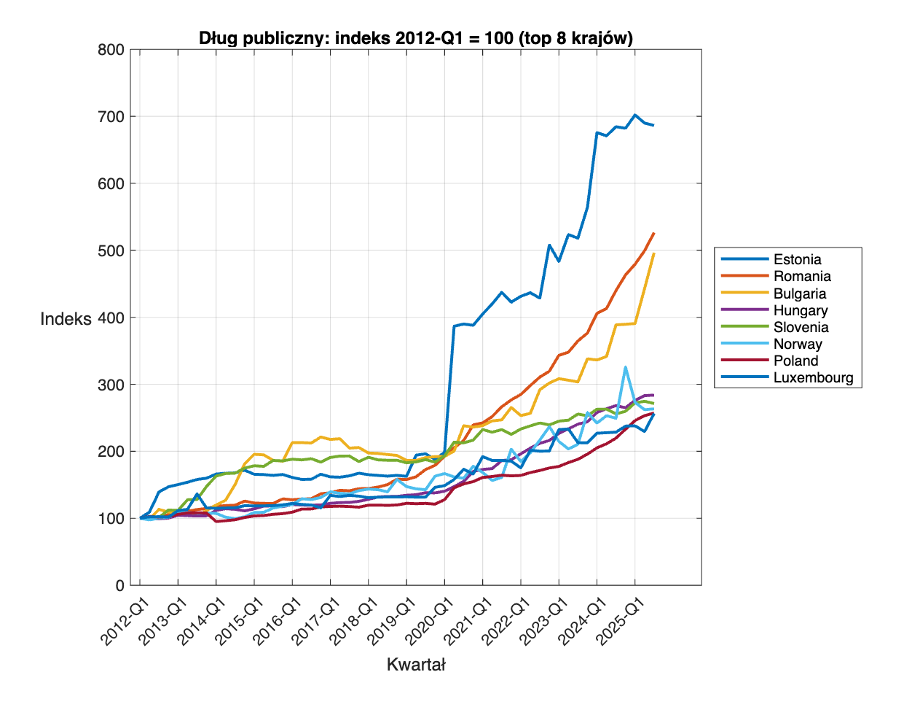
\includegraphics[width=\textwidth]{phts/4/png/4.1.png}
    \caption{Dług publiczny: indeks 2012-Q1 = 100 dla 8 krajów o największym wzroście.}
\end{figure}

Wykres przedstawia kraje, w których indeks długu publicznego wzrósł najmocniej względem początku analizowanego okresu.
Najbardziej wyróżnia się Estonia, której indeks w ostatnich latach osiąga wartości bliskie 700, co oznacza kilkukrotny wzrost względem 2012-Q1.
Silny wzrost widoczny jest również w Rumunii oraz Bułgarii, szczególnie po roku 2020.

Na wykresie wyraźnie widać, że dla większości państw tempo wzrostu zadłużenia przyspieszyło po okresie pandemicznym.
Nie oznacza to jednak, że państwa te mają największy dług nominalnie, tylko że ich dług wzrósł najbardziej względem własnego poziomu początkowego.


\subsubsection{Skumulowana zmiana długu od początku próby}
\begin{figure}[H]
    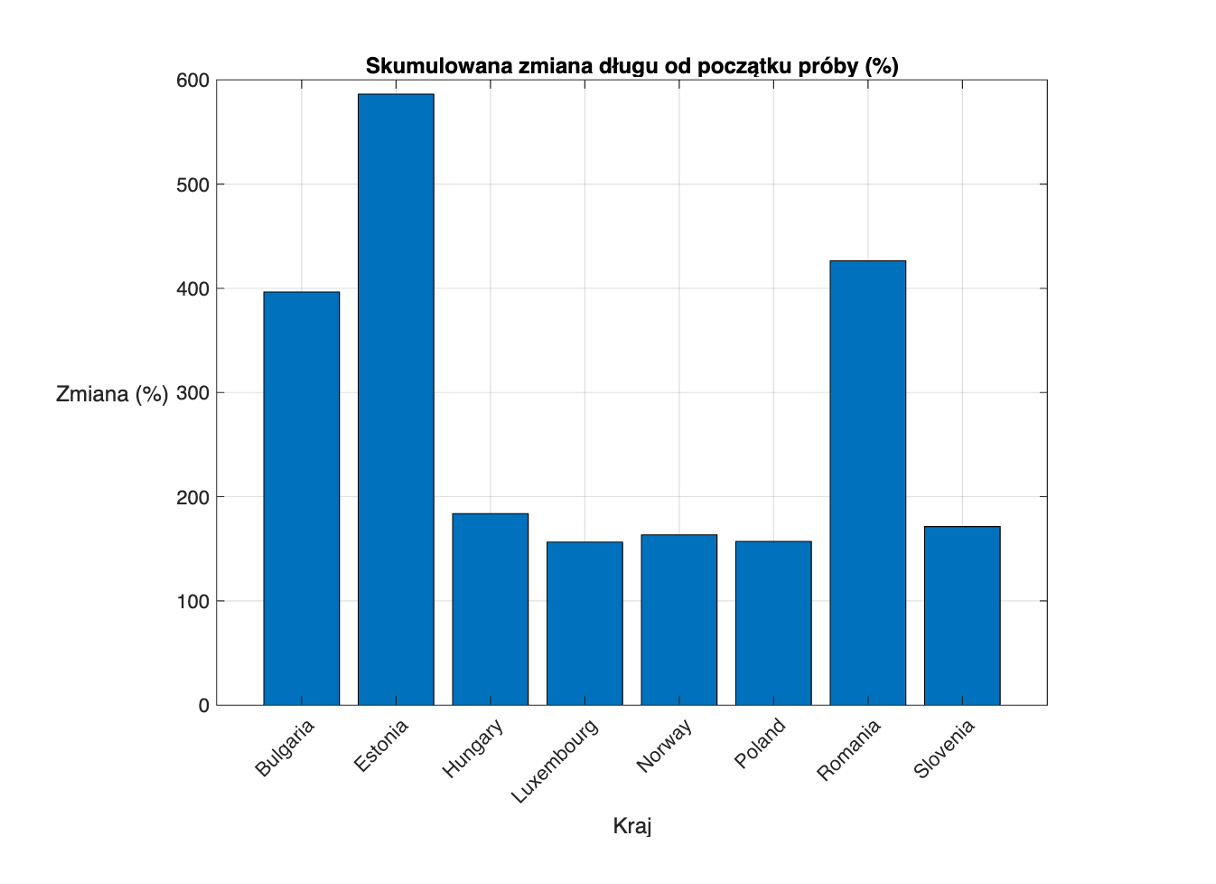
\includegraphics[width=\textwidth]{phts/4/png/4.2.png}
    \caption{Skumulowana zmiana długu publicznego od początku próby.}
\end{figure}

Wykres przedstawia skumulowaną zmianę długu publicznego od początku badanego okresu.
Najsilniejszy wzrost odnotowano w Estonii, gdzie skumulowana zmiana wyniosła około 586\%.
Wysokie wartości występują również w Rumunii oraz Bułgarii.

Polska znajduje się w grupie krajów z wyraźnym wzrostem długu, jednak nie osiąga wartości tak wysokich jak Estonia czy Rumunia.
Wizualizacja potwierdza obserwacje z wykresu indeksowego: kraje Europy Środkowo-Wschodniej należą do państw o największym względnym wzroście długu publicznego w analizowanym okresie.


\subsubsection{Indeks długu publicznego dla wybranych dużych gospodarek}
\begin{figure}[H]
    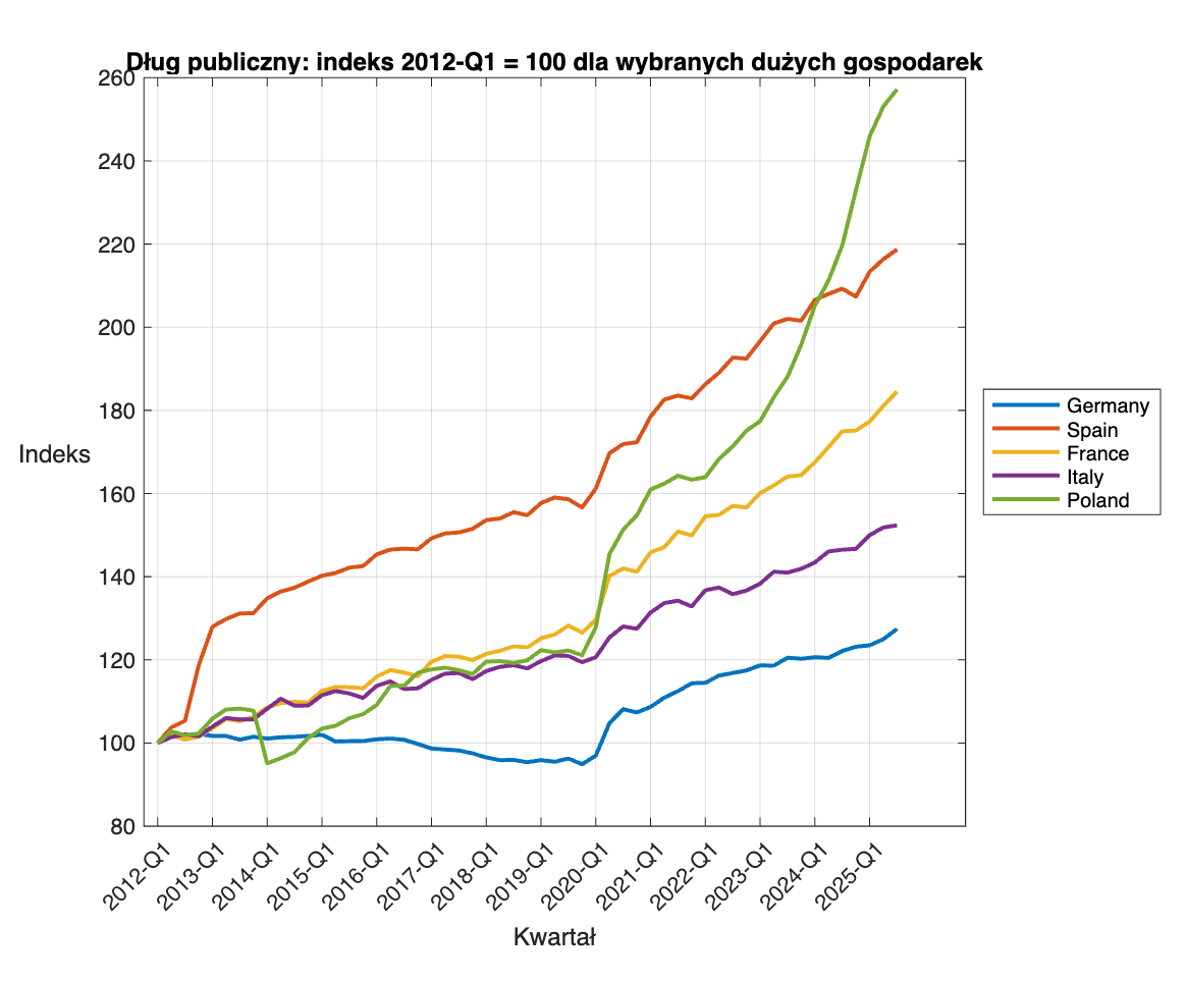
\includegraphics[width=\textwidth]{phts/4/png/4.3.png}
    \caption{Dług publiczny: indeks 2012-Q1 = 100 dla wybranych dużych gospodarek.}
\end{figure}

Wykres porównuje indeks długu publicznego dla wybranych dużych gospodarek europejskich: Niemiec, Hiszpanii, Francji, Włoch oraz Polski.
Największy wzrost w tej grupie widoczny jest dla Polski, szczególnie po roku 2020.
Hiszpania również osiąga wysokie wartości indeksu, ale jej wzrost był bardziej stopniowy.

Niemcy wyróżniają się najniższą wartością indeksu w tej grupie.
Ich dług publiczny przez dużą część analizowanego okresu pozostawał blisko poziomu początkowego, a wyraźniejszy wzrost pojawił się dopiero po 2020 roku.
W porównaniu z pozostałymi dużymi gospodarkami Polska cechuje się więc szczególnie mocnym wzrostem długu względem początku próby.


\subsubsection{Dynamika długu rok do roku dla krajów o najsilniejszych bieżących zmianach}
\begin{figure}[H]
    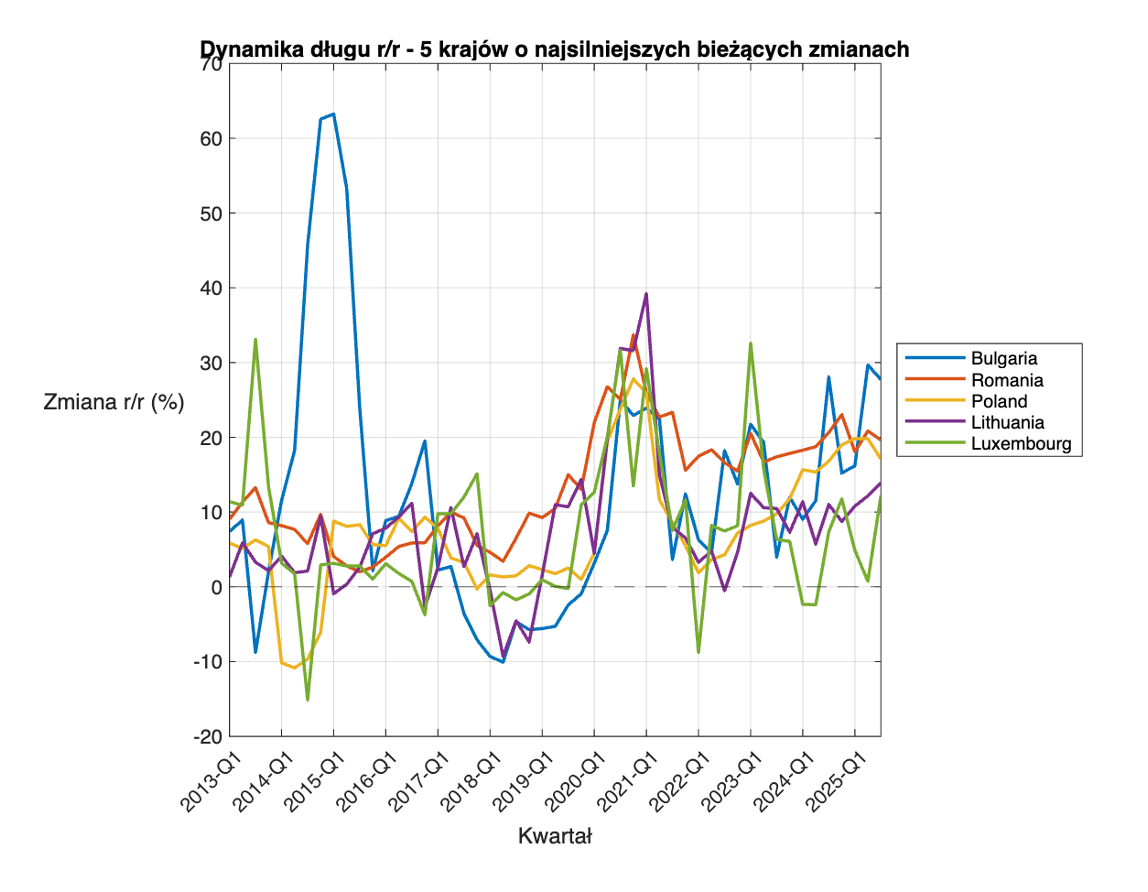
\includegraphics[width=\textwidth]{phts/4/png/4.4.png}
    \caption{Dynamika długu rok do roku - 5 krajów o najsilniejszych bieżących zmianach.}
\end{figure}

Wizualizacja pokazuje dynamikę długu publicznego rok do roku dla pięciu krajów o najsilniejszych bieżących zmianach.
Najbardziej gwałtowne wahania widoczne są dla Bułgarii, która w niektórych okresach osiągała bardzo wysokie dodatnie wartości dynamiki.
Wyraźne skoki można zauważyć również dla Rumunii, Polski, Litwy oraz Luksemburga.

Na wykresie dobrze widać, że dynamika długu jest znacznie bardziej chaotyczna niż sam indeks długu.
Wartość indeksu może rosnąć stosunkowo płynnie, natomiast dynamika rok do roku pokazuje krótkookresowe przyspieszenia i spowolnienia zmian zadłużenia.


\subsubsection{Najwyższa zmienność dynamiki długu rok do roku}
\begin{figure}[H]
    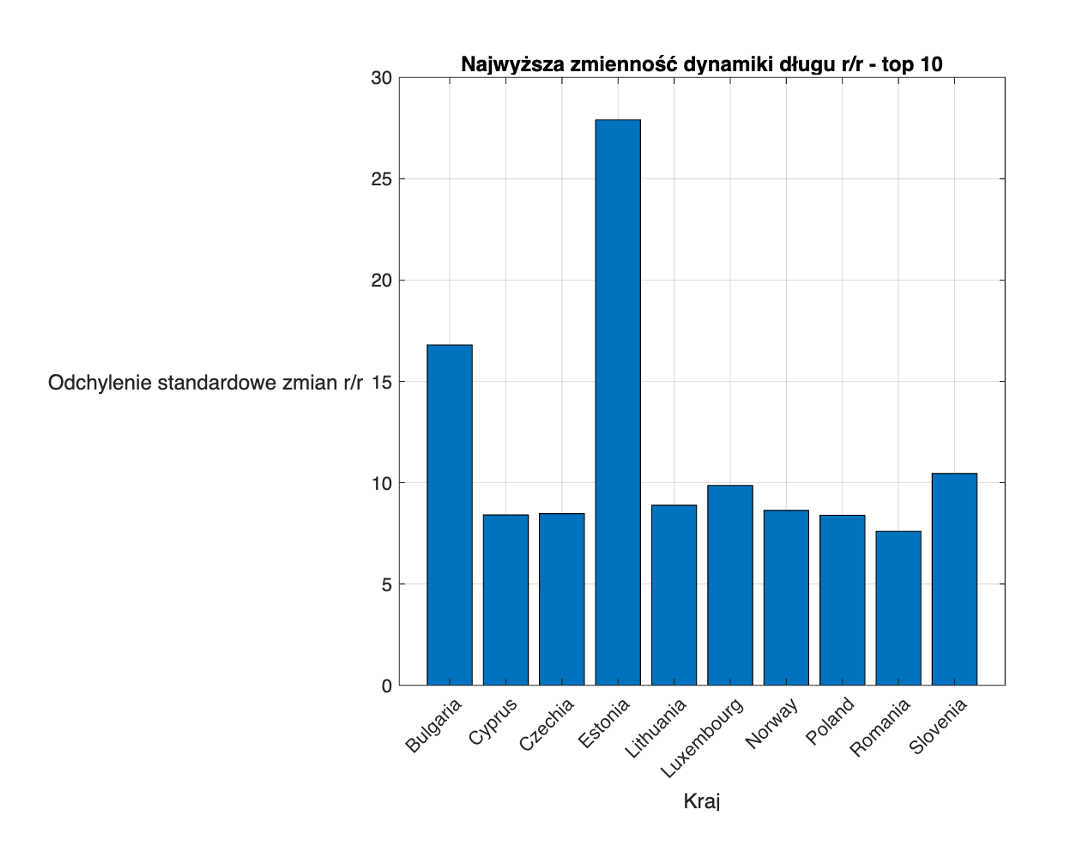
\includegraphics[width=\textwidth]{phts/4/png/4.5.png}
    \caption{Najwyższa zmienność dynamiki długu publicznego rok do roku - top 10 krajów.}
\end{figure}

Wykres przedstawia kraje o największym odchyleniu standardowym dynamiki długu rok do roku.
Największą zmienność wykazuje Estonia, co oznacza, że tempo zmian jej długu publicznego było najmniej stabilne spośród analizowanych państw.
Wysoka zmienność widoczna jest również dla Bułgarii oraz Słowenii.

Odchylenie standardowe nie pokazuje samego poziomu długu, lecz niestabilność jego zmian.
Kraj może mieć relatywnie niski poziom długu nominalnego, ale jednocześnie bardzo dynamiczne i nieregularne zmiany względem poprzednich lat.


\subsubsection{Heatmap indeksu długu publicznego}
\begin{figure}[H]
    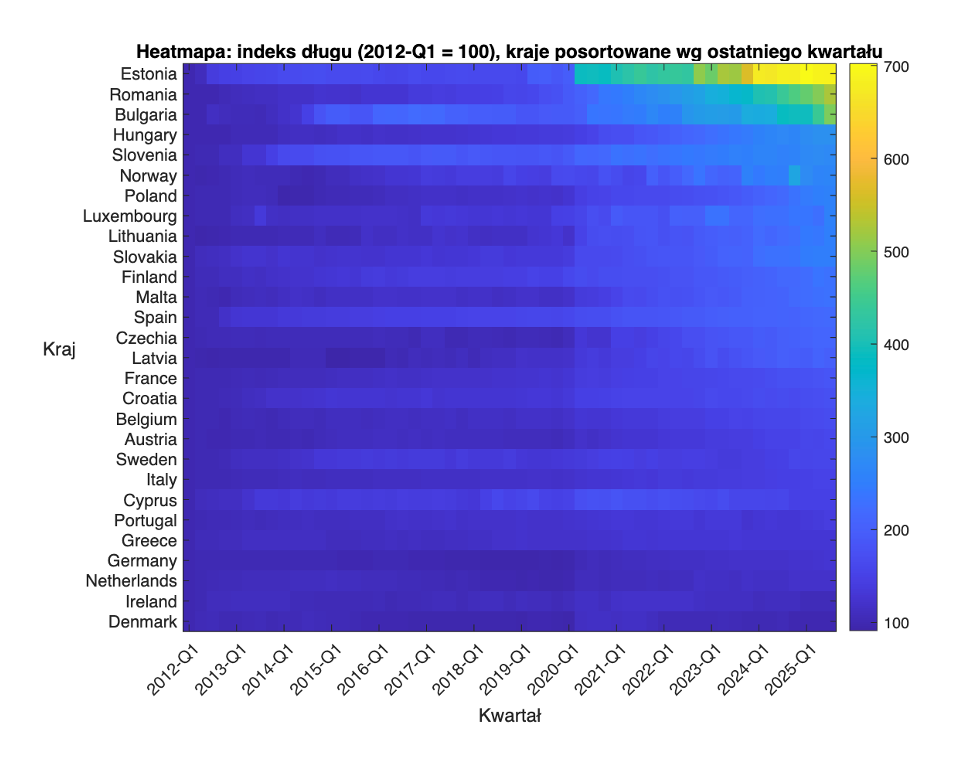
\includegraphics[width=\textwidth]{phts/4/png/4.6.png}
    \caption{Heatmapa indeksu długu publicznego względem 2012-Q1, kraje posortowane według ostatniego kwartału.}
\end{figure}

Heatmapa przedstawia przebieg indeksu długu publicznego dla wszystkich analizowanych krajów.
Kolory pozwalają szybko zauważyć, które kraje przez większość okresu utrzymywały się blisko punktu startowego, a które weszły na wyraźnie wyższe poziomy zadłużenia.

Najsilniejsze wartości widoczne są w górnej części wykresu, m.in. dla Estonii, Rumunii i Bułgarii.
W ich przypadku kolory stają się coraz jaśniejsze w końcowej części szeregu, co oznacza wzrost indeksu długu.
Z kolei kraje znajdujące się niżej na wykresie, takie jak Dania, Irlandia czy Holandia, zachowują bardziej stabilny poziom indeksu.


\subsubsection{Ostatni kwartał względem średniej z całego okresu}
\begin{figure}[H]
    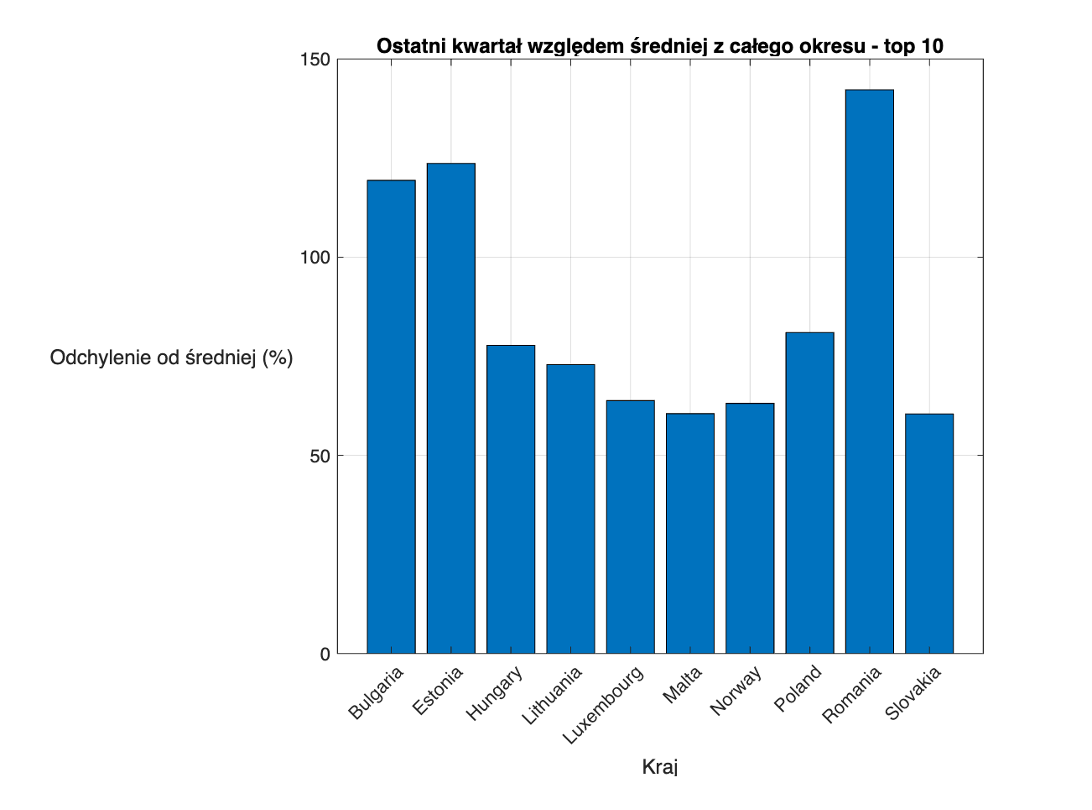
\includegraphics[width=\textwidth]{phts/4/png/4.7.png}
    \caption{Ostatni kwartał względem średniej z całego okresu - top 10 krajów.}
\end{figure}

Wykres pokazuje, o ile ostatnia dostępna wartość indeksu długu różni się od średniej wartości indeksu dla danego kraju z całego badanego okresu.
Największe dodatnie odchylenie występuje w Rumunii, Estonii oraz Bułgarii.
Oznacza to, że obecny poziom zadłużenia tych państw jest wyraźnie wyższy niż ich przeciętny poziom z lat 2012--2025.

Taka wizualizacja pozwala szybko wskazać kraje, które znajdują się obecnie na relatywnie wysokiej ścieżce zadłużenia.
Warto zauważyć, że w zestawieniu znajduje się również Polska, co oznacza, że ostatni poziom długu publicznego jest znacząco wyższy od średniej z całego okresu.


\subsubsection{Średni indeks długu w grupach krajów}
\begin{figure}[H]
    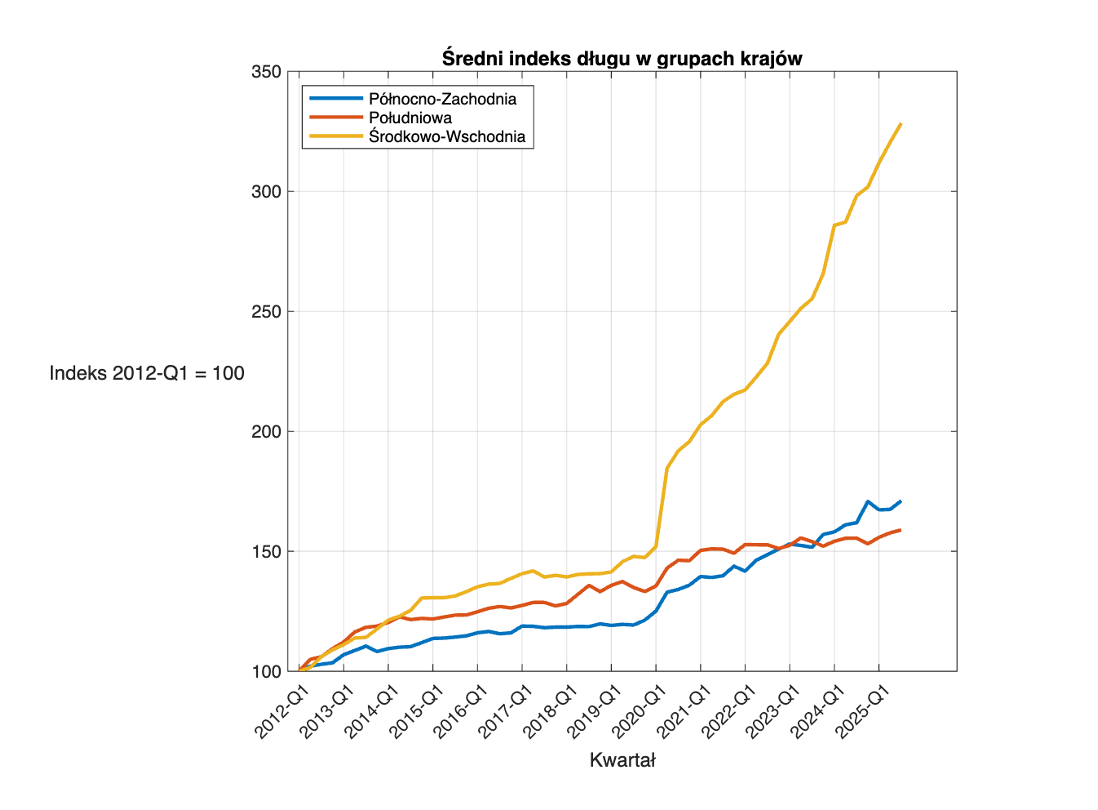
\includegraphics[width=\textwidth]{phts/4/png/4.8.png}
    \caption{Średni indeks długu publicznego w grupach krajów.}
\end{figure}

Na potrzeby analizy kraje zostały podzielone na trzy orientacyjne grupy: Europę Północno-Zachodnią, Europę Południową oraz Europę Środkowo-Wschodnią.
Wizualizacja pokazuje średnią wartość indeksu długu w każdej z tych grup.

Największy wzrost średniego indeksu widoczny jest w grupie państw Europy Środkowo-Wschodniej.
Do około 2020 roku różnice między grupami były zauważalne, ale nie aż tak duże. Po 2020 roku krzywa dla Europy Środkowo-Wschodniej zaczyna rosnąć znacznie szybciej.
Sugeruje to, że w tej grupie krajów dług publiczny wzrastał relatywnie mocniej niż w Europie Południowej oraz Północno-Zachodniej.


\subsection{Wnioski}
\begin{enumerate}
    \item Najsilniejszy wzrost nominalnego długu od początku próby odnotowano w Estonii, gdzie skumulowana zmiana wyniosła około 586.3\%.
    \item Największą zmienność dynamiki rok do roku miała Estonia, co oznacza, że jej zadłużenie zmieniało się najbardziej nieregularnie.
    \item Najbardziej stabilny przebieg dynamiki rok do roku występował we Włoszech.
    \item Najwyższa ostatnia dynamika rok do roku wystąpiła w Bułgarii i wyniosła około 27.7\%.
    \item Najsłabsza ostatnia dynamika rok do roku wystąpiła na Cyprze i wyniosła około -5.0\%.
    \item Po 2020 roku w wielu krajach widoczne jest przyspieszenie wzrostu długu publicznego, szczególnie w państwach Europy Środkowo-Wschodniej.
    \item Polska, w porównaniu z wybranymi dużymi gospodarkami europejskimi, charakteryzuje się jednym z mocniejszych wzrostów indeksu długu względem 2012-Q1.
\end{enumerate}


\newpage
\section{Misje kosmiczne (MATLAB)}

Przygotowane przez: Jan Domański

\subsection{Źródło danych}
\href{https://www.kaggle.com/datasets/agirlcoding/all-space-missions-from-1957}
{Kaggle - All Space Missions From 1957} \\
\url{https://www.kaggle.com/datasets/agirlcoding/all-space-missions-from-1957}

\subsection{Opis zbioru i istotnych pojęć}
\begin{itemize}
    \item Zbiór przedstawia globalne misje kosmiczne realizowane przez różne kraje, firmy oraz organizacje;
    \item Dane obejmują okres od 1957 do 2020 roku;
    \item Ostatnia aktualizacja wykorzystanego zbioru miała miejsce 13/08/2020;
    \item Dane kosztowe są dostępne tylko dla części misji, dlatego analiza kosztów opiera się na podzbiorze danych;
    \item Dekada 2020 nie jest pełna, dlatego została pominięta w analizie dekad;
    \item \textbf{Misja kosmiczna} - pojedyncze przedsięwzięcie związane ze startem rakiety lub pojazdu kosmicznego;
    \item \textbf{Status misji} - końcowy wynik misji, np. sukces, porażka, częściowa porażka lub porażka przedstartowa;
    \item \textbf{Skuteczność misji} - odsetek misji zakończonych sukcesem względem wszystkich misji w danej grupie;
    \item \textbf{Lokalizacja startu} - państwo lub obszar, z którego przeprowadzono start misji;
    \item \textbf{Firma / organizacja} - podmiot odpowiedzialny za przeprowadzenie misji, np. agencja kosmiczna, firma prywatna lub organizacja państwowa.
\end{itemize}


\subsection{Wizualizacje zbioru}

\subsubsection{Liczba misji kosmicznych w czasie}
\begin{figure}[H]
    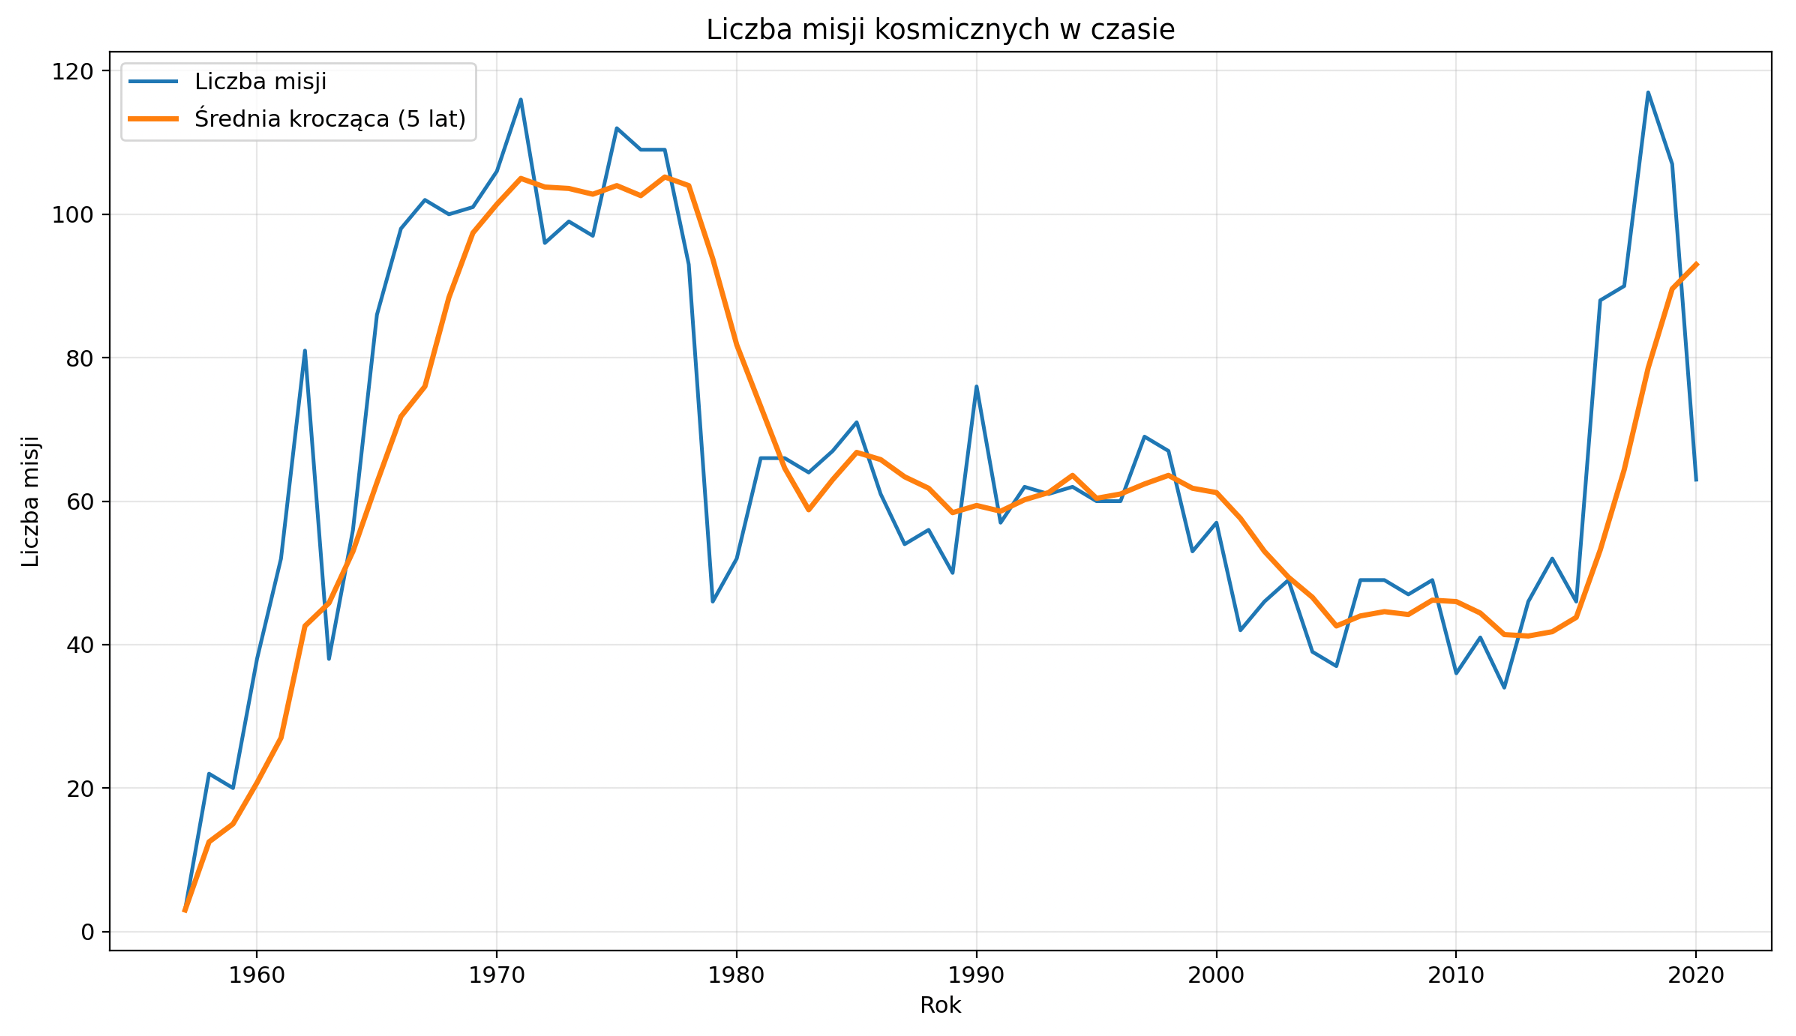
\includegraphics[width=\textwidth]{phts/5/png/5.1.png}
    \caption{Liczba misji kosmicznych w czasie.}
\end{figure}

Wykres przedstawia liczbę misji kosmicznych w poszczególnych latach oraz pięcioletnią średnią kroczącą.
Największa aktywność widoczna jest w okresie zimnej wojny, szczególnie od drugiej połowy lat 60. do końca lat 70.
W tym czasie liczba misji w wielu latach przekraczała 100 rocznie.

Po zakończeniu najbardziej intensywnego okresu rywalizacji kosmicznej liczba misji wyraźnie spadła i przez długi czas utrzymywała się na niższym poziomie.
Ponowny wzrost aktywności widoczny jest w drugiej połowie lat 2010., co można wiązać z rozwojem nowych technologii, większą rolą firm prywatnych oraz wzrostem zainteresowania komercyjnymi startami kosmicznymi.


\subsubsection{Liczba misji kosmicznych według dekad}
\begin{figure}[H]
    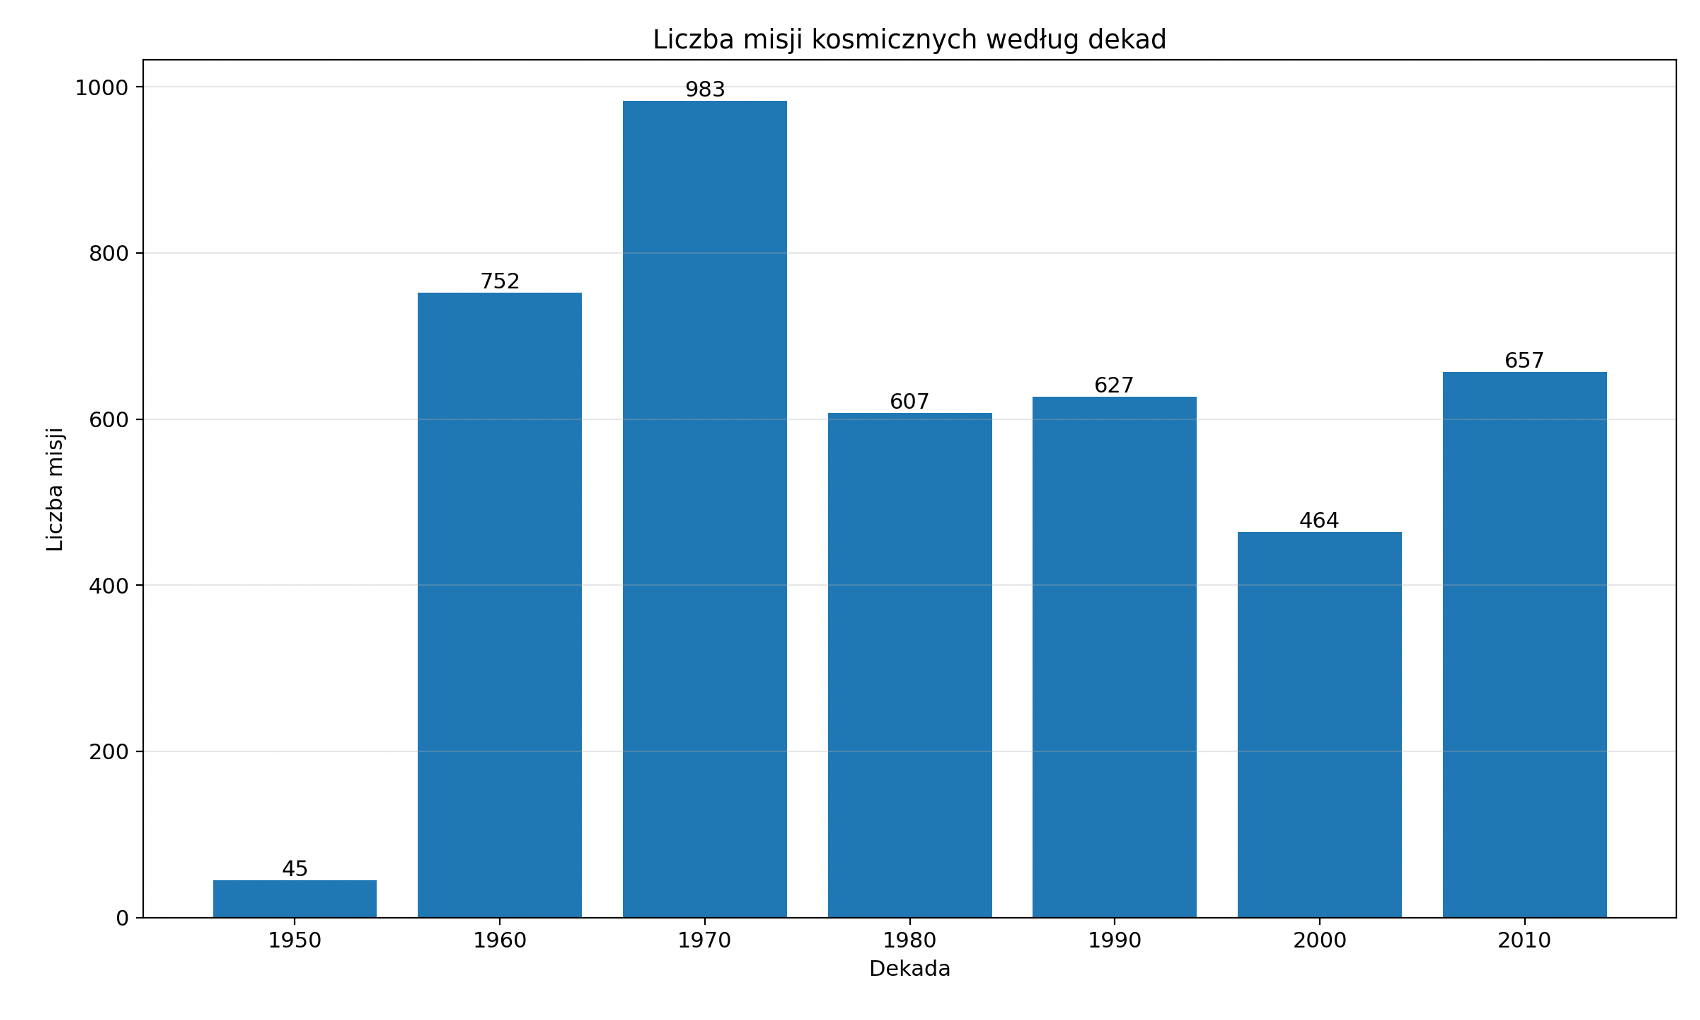
\includegraphics[width=\textwidth]{phts/5/png/5.2.png}
    \caption{Liczba misji kosmicznych według dekad.}
\end{figure}

Na wykresie pokazano łączną liczbę misji kosmicznych w poszczególnych dekadach.
Najwięcej misji przeprowadzono w latach 70., gdzie liczba startów wyniosła 983.
Bardzo wysoka aktywność widoczna jest również w latach 60., z liczbą 752 misji.

Po latach 70. nastąpił spadek liczby misji, szczególnie widoczny w dekadzie 2000.
W latach 2010. liczba misji ponownie wzrosła do 657, co pokazuje odbudowę aktywności sektora kosmicznego.
Dekada 2020 nie została tutaj uwzględniona, ponieważ w zbiorze nie jest kompletna.


\subsubsection{Top 10 krajów według liczby misji}
\begin{figure}[H]
    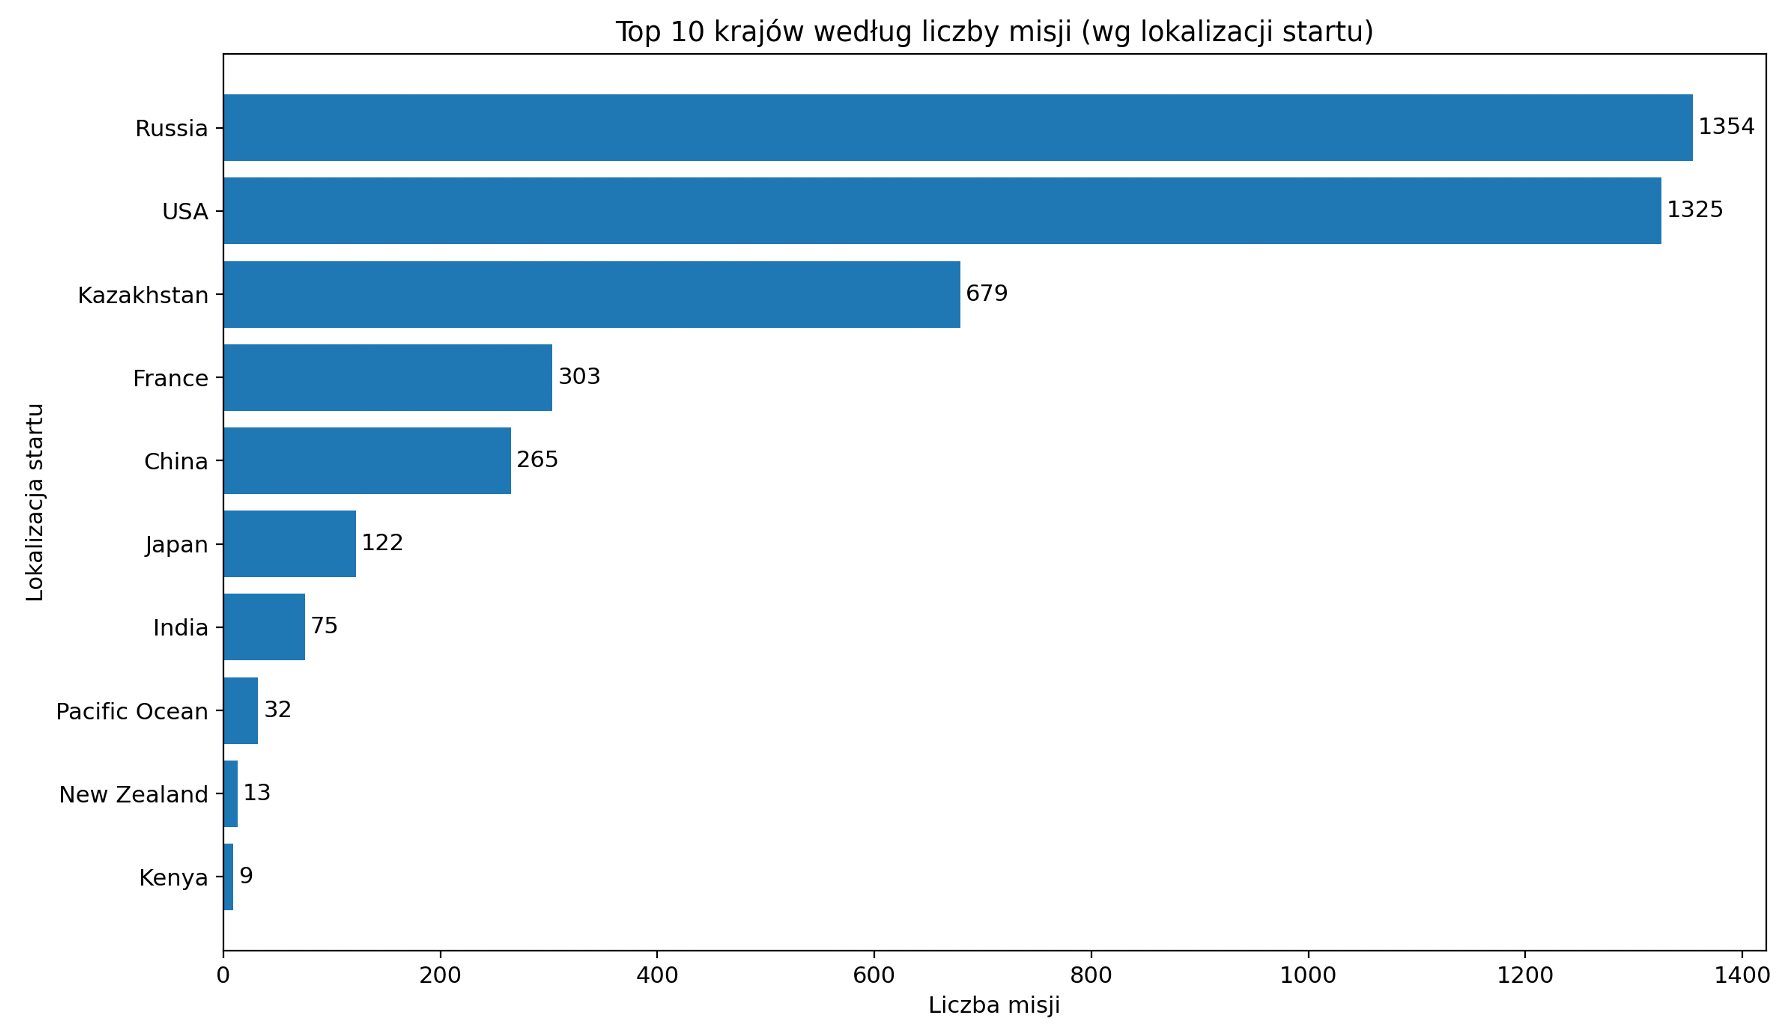
\includegraphics[width=\textwidth]{phts/5/png/5.3.png}
    \caption{Top 10 krajów według liczby misji kosmicznych według lokalizacji startu.}
\end{figure}

Wizualizacja przedstawia kraje i lokalizacje startu z największą liczbą misji kosmicznych.
Najwięcej misji przeprowadzono z Rosji oraz Stanów Zjednoczonych - odpowiednio 1354 i 1325.
Są to zdecydowanie dominujące lokalizacje w całym zbiorze.

Na trzecim miejscu znajduje się Kazachstan z 679 misjami, co wynika głównie z historycznego i strategicznego znaczenia kosmodromu Bajkonur.
Pozostałe kraje, takie jak Francja, Chiny, Japonia czy Indie, mają znacznie mniejszą liczbę startów, ale nadal stanowią istotną część globalnej aktywności kosmicznej.


\subsubsection{Top 10 firm i organizacji według liczby misji}
\begin{figure}[H]
    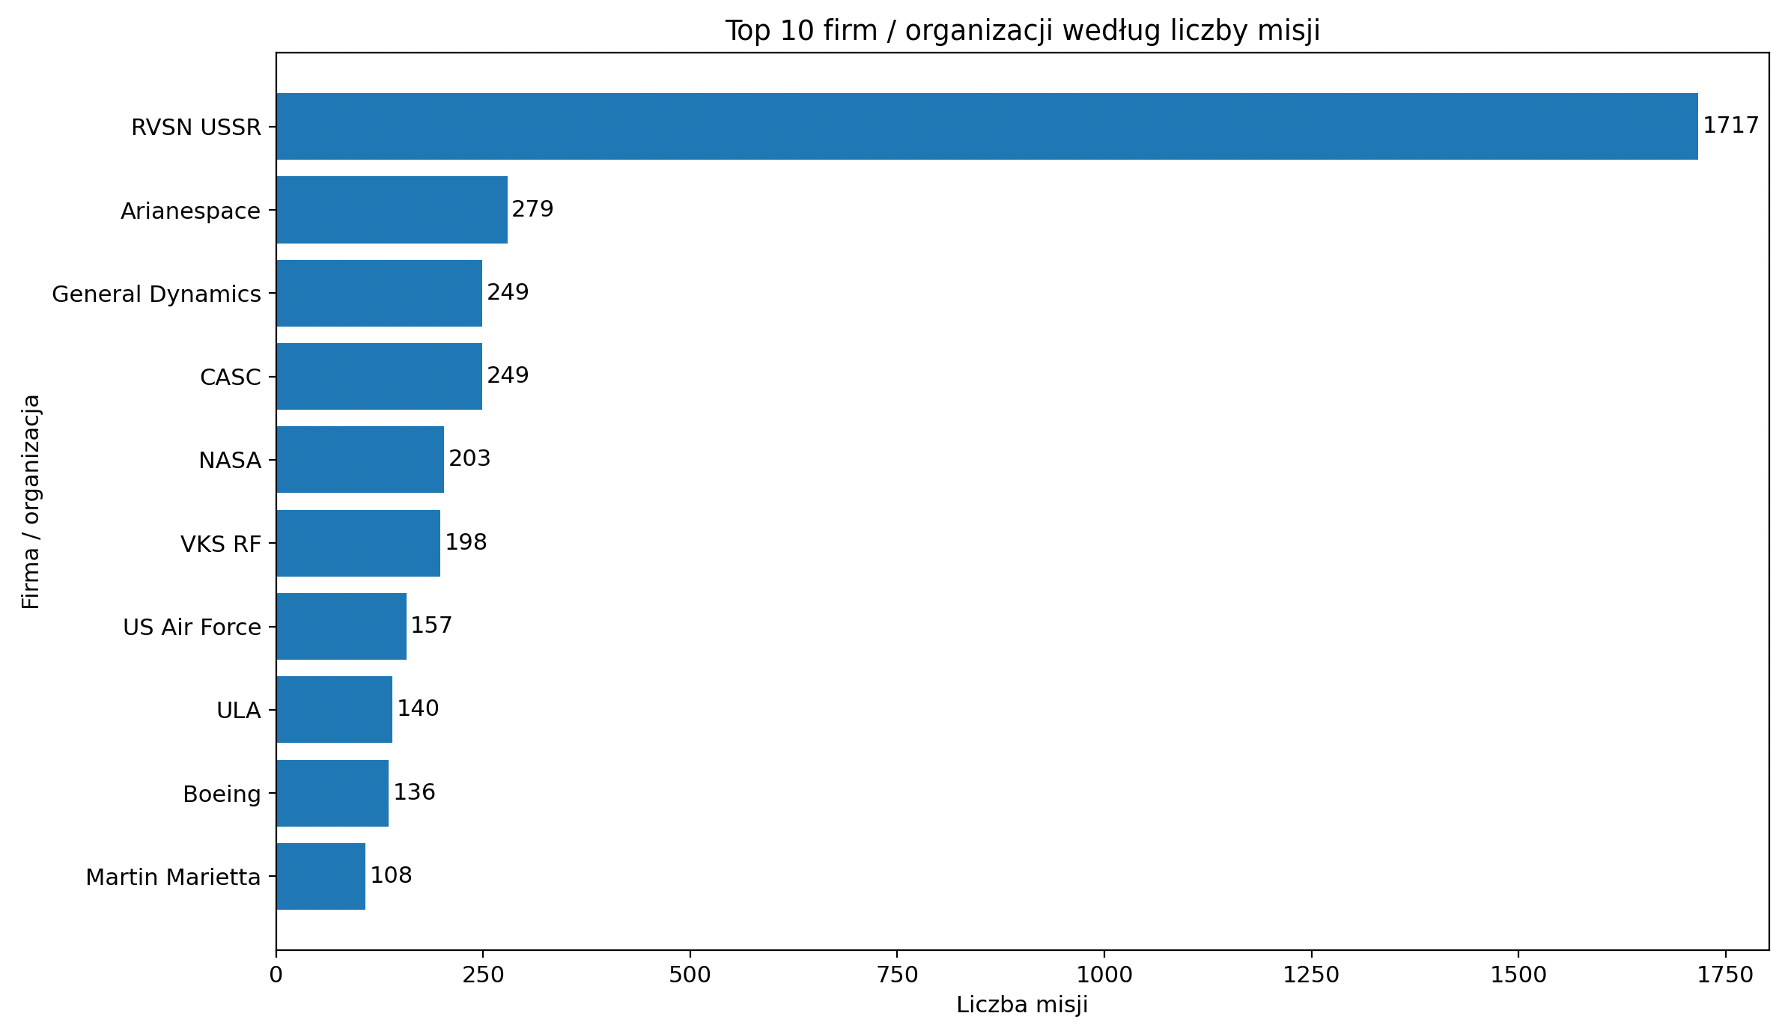
\includegraphics[width=\textwidth]{phts/5/png/5.4.png}
    \caption{Top 10 firm i organizacji według liczby misji kosmicznych.}
\end{figure}

Wykres przedstawia organizacje i firmy, które przeprowadziły największą liczbę misji kosmicznych.
Zdecydowanie dominuje RVSN USSR z 1717 misjami, czyli z wynikiem wielokrotnie większym niż kolejne organizacje w zestawieniu.
Tak duża przewaga dobrze pokazuje skalę radzieckiej aktywności kosmicznej w analizowanym okresie.

Na kolejnych miejscach znajdują się m.in. Arianespace, General Dynamics, CASC oraz NASA.
Ich wyniki są znacznie niższe niż RVSN USSR, ale pokazują zróżnicowanie podmiotów odpowiedzialnych za misje: od organizacji państwowych, przez agencje kosmiczne, po przedsiębiorstwa komercyjne.


\subsubsection{Aktywność top 5 firm w czasie}
\begin{figure}[H]
    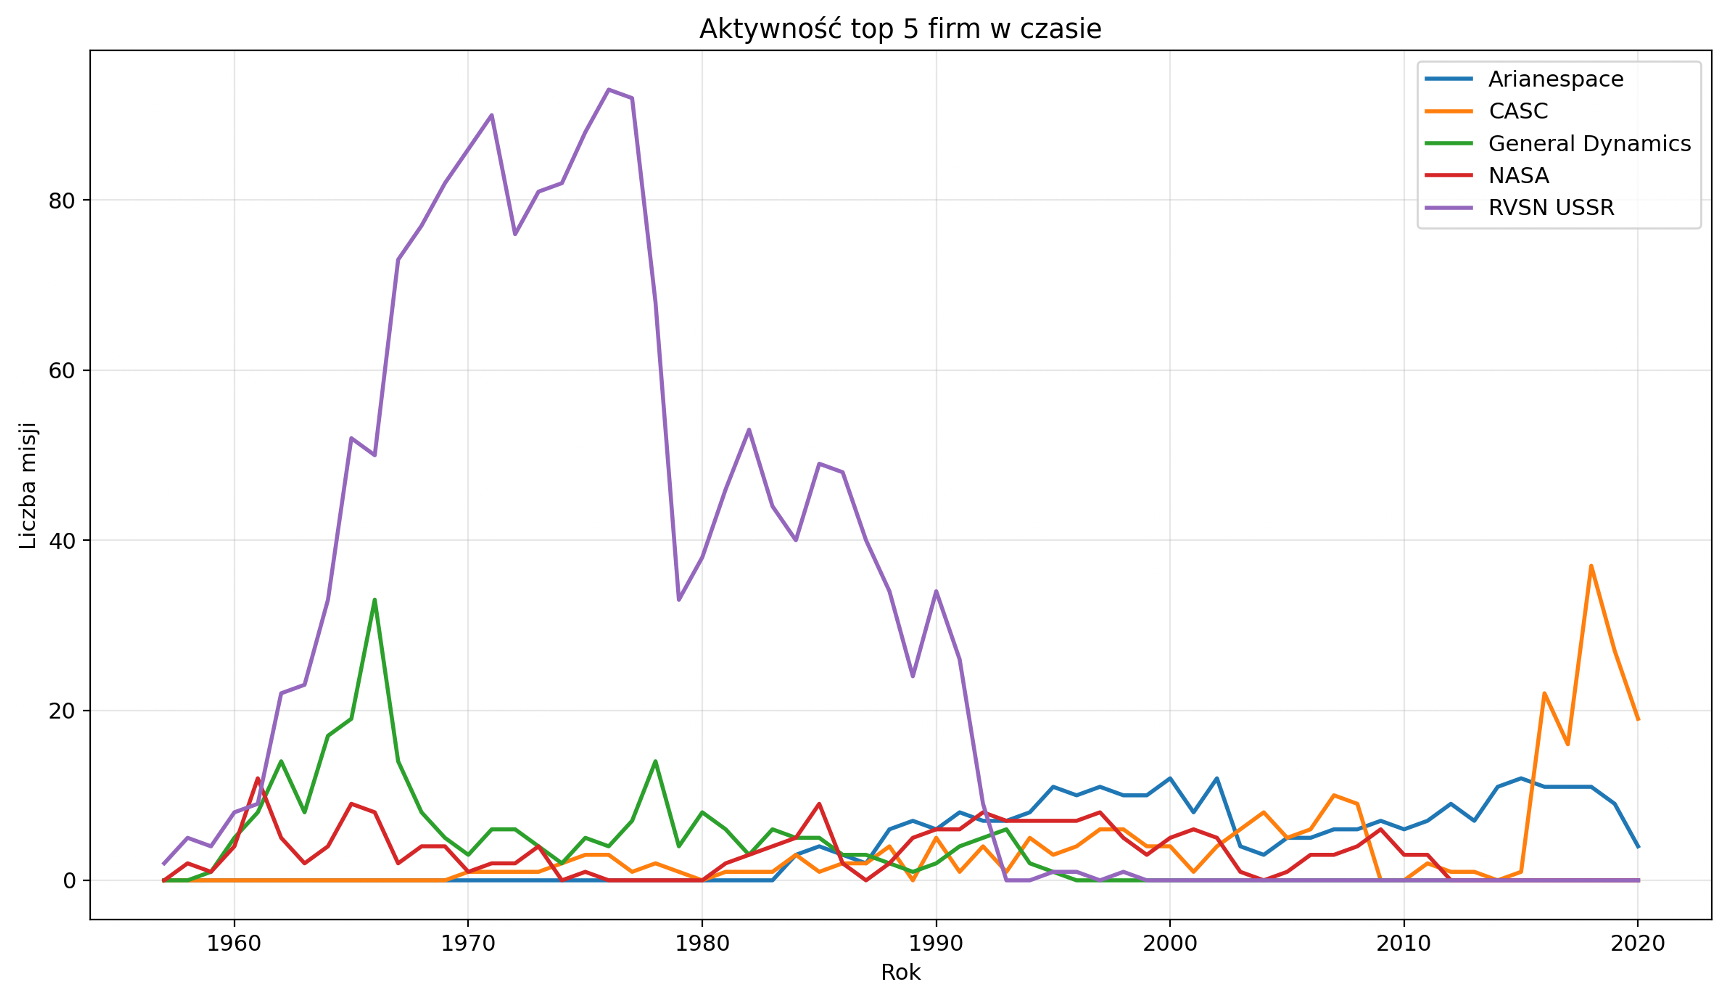
\includegraphics[width=\textwidth]{phts/5/png/5.5.png}
    \caption{Aktywność top 5 firm i organizacji w czasie.}
\end{figure}

Wykres pokazuje, jak zmieniała się aktywność pięciu najważniejszych organizacji w czasie.
Najbardziej charakterystyczny jest przebieg RVSN USSR, które osiągało bardzo wysoką liczbę misji w latach 60. i 70., a następnie jego aktywność gwałtownie spadła.
Widać więc silną koncentrację radzieckiej aktywności kosmicznej w określonym okresie historycznym.

W późniejszych latach większą rolę zaczęły odgrywać inne organizacje, takie jak Arianespace, NASA oraz CASC.
Szczególnie widoczny jest wzrost aktywności CASC w końcowej części szeregu czasowego, co wskazuje na rosnące znaczenie Chin w sektorze kosmicznym.


\subsubsection{Sezonowość startów kosmicznych według miesięcy}
\begin{figure}[H]
    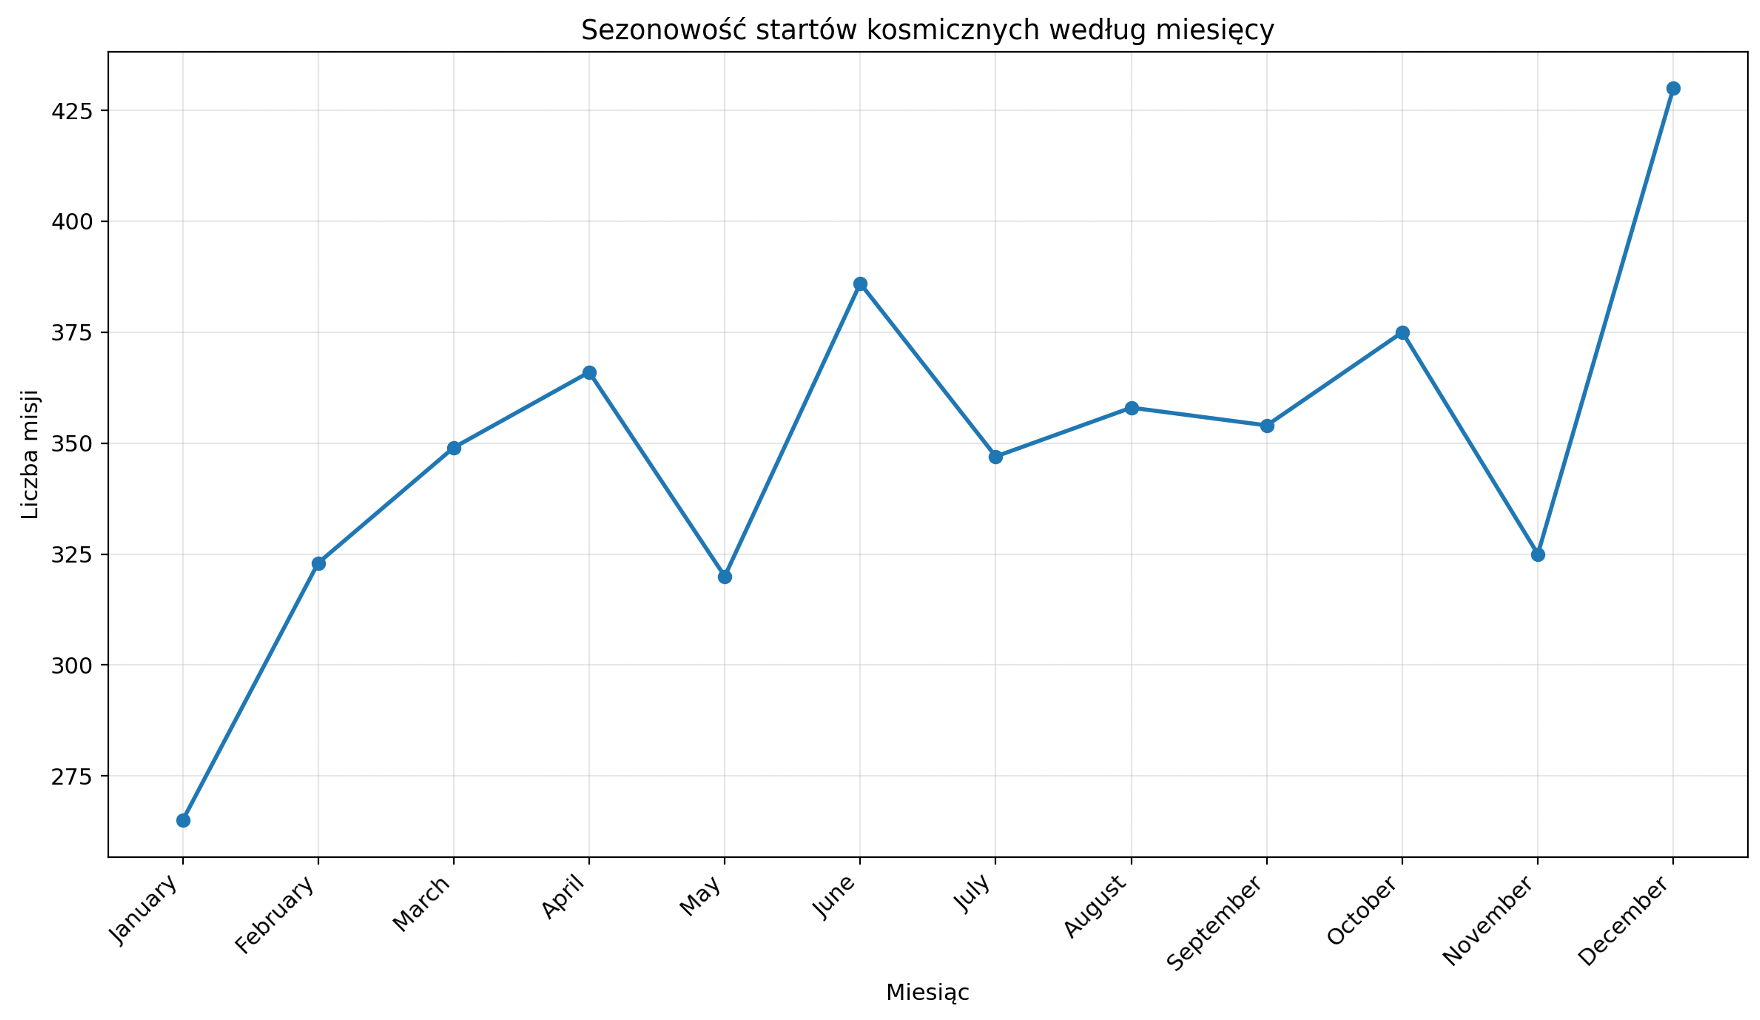
\includegraphics[width=\textwidth]{phts/5/png/5.6.png}
    \caption{Sezonowość startów kosmicznych według miesięcy.}
\end{figure}

Wykres przedstawia liczbę misji kosmicznych w podziale na miesiące.
Najwięcej startów odnotowano w grudniu, a wysokie wartości widoczne są również w czerwcu i październiku.
Najmniejsza liczba misji przypada natomiast na styczeń.

Taki rozkład może sugerować istnienie sezonowości w planowaniu startów, jednak różnice między miesiącami nie powinny być interpretowane wyłącznie jako efekt warunków pogodowych.
Na liczbę misji wpływają również harmonogramy techniczne, budżetowe, polityczne oraz organizacyjne.


\subsubsection{Rozkład wyników misji}
\begin{figure}[H]
    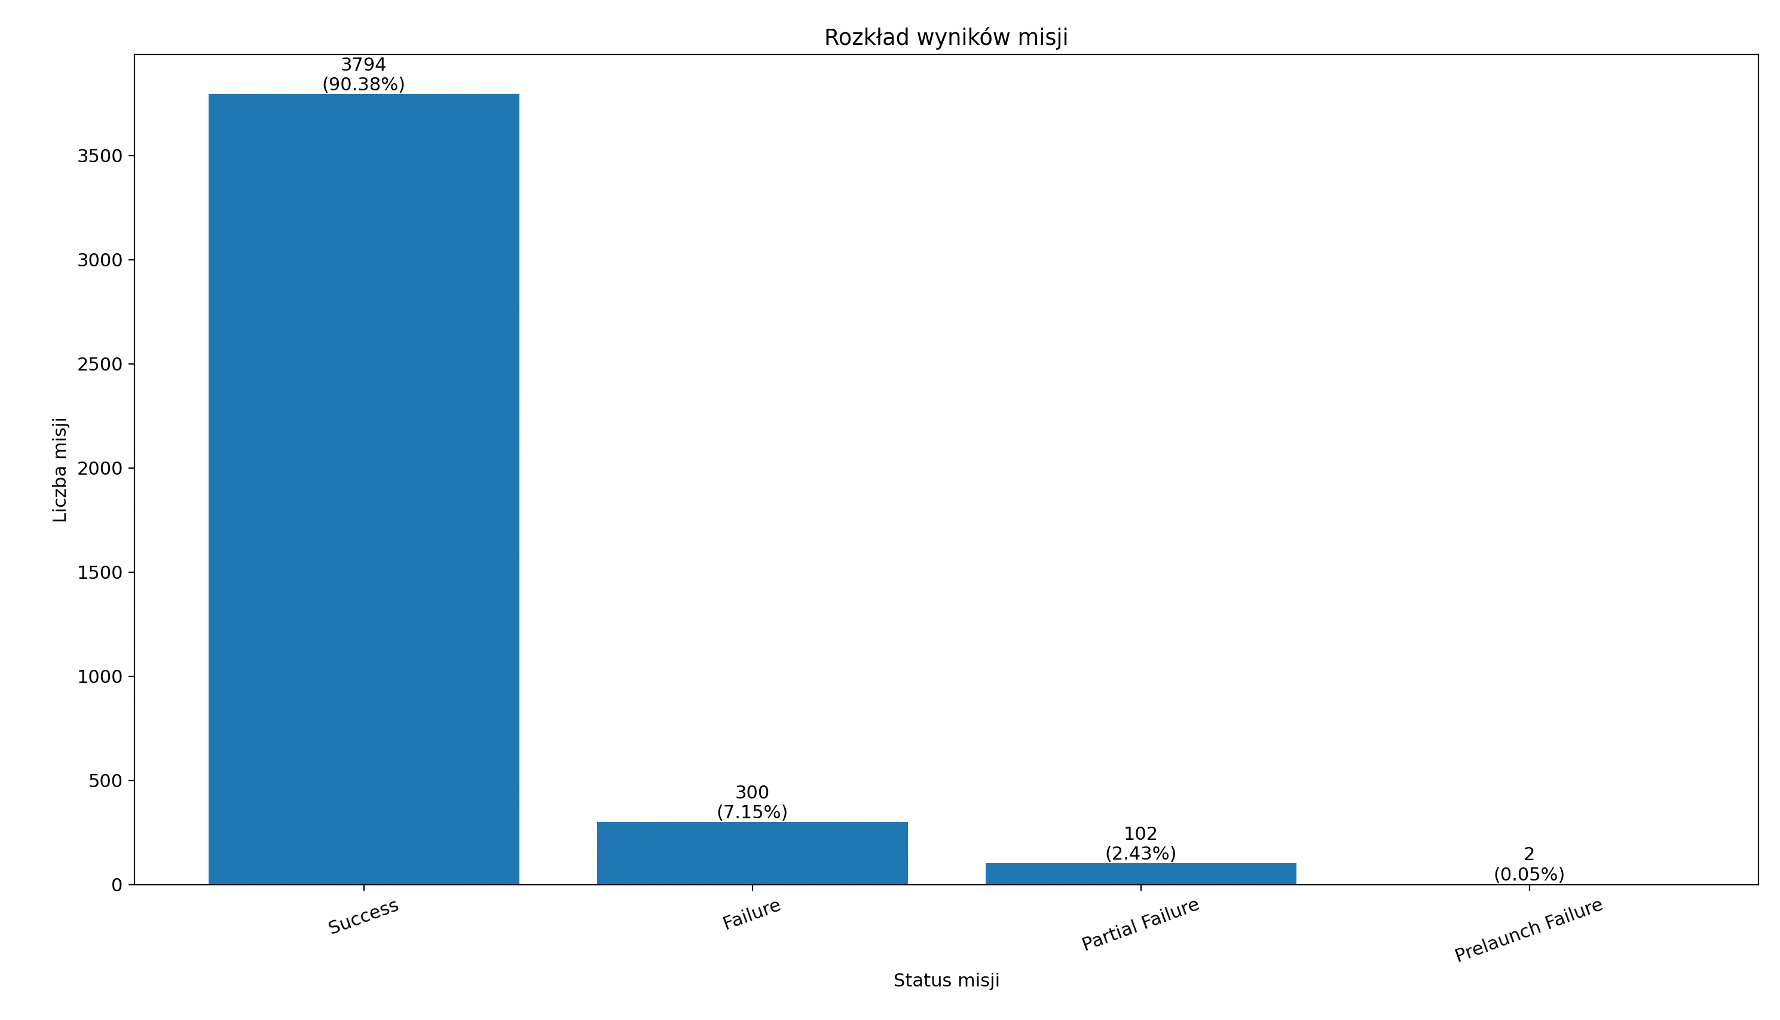
\includegraphics[width=\textwidth]{phts/5/png/5.7.png}
    \caption{Rozkład wyników misji kosmicznych.}
\end{figure}

Wizualizacja pokazuje, jak często misje kończyły się poszczególnymi statusami.
Zdecydowana większość misji zakończyła się sukcesem - 3794 przypadki, czyli około 90.38\% wszystkich misji.
Porażki stanowią znacznie mniejszą część zbioru: 300 misji, czyli około 7.15\%.

Częściowe porażki oraz porażki przedstartowe pojawiają się bardzo rzadko.
Oznacza to, że mimo wysokiego poziomu trudności technicznej misji kosmicznych, większość zarejestrowanych startów zakończyła się powodzeniem.


\subsubsection{Skuteczność misji w czasie}
\begin{figure}[H]
    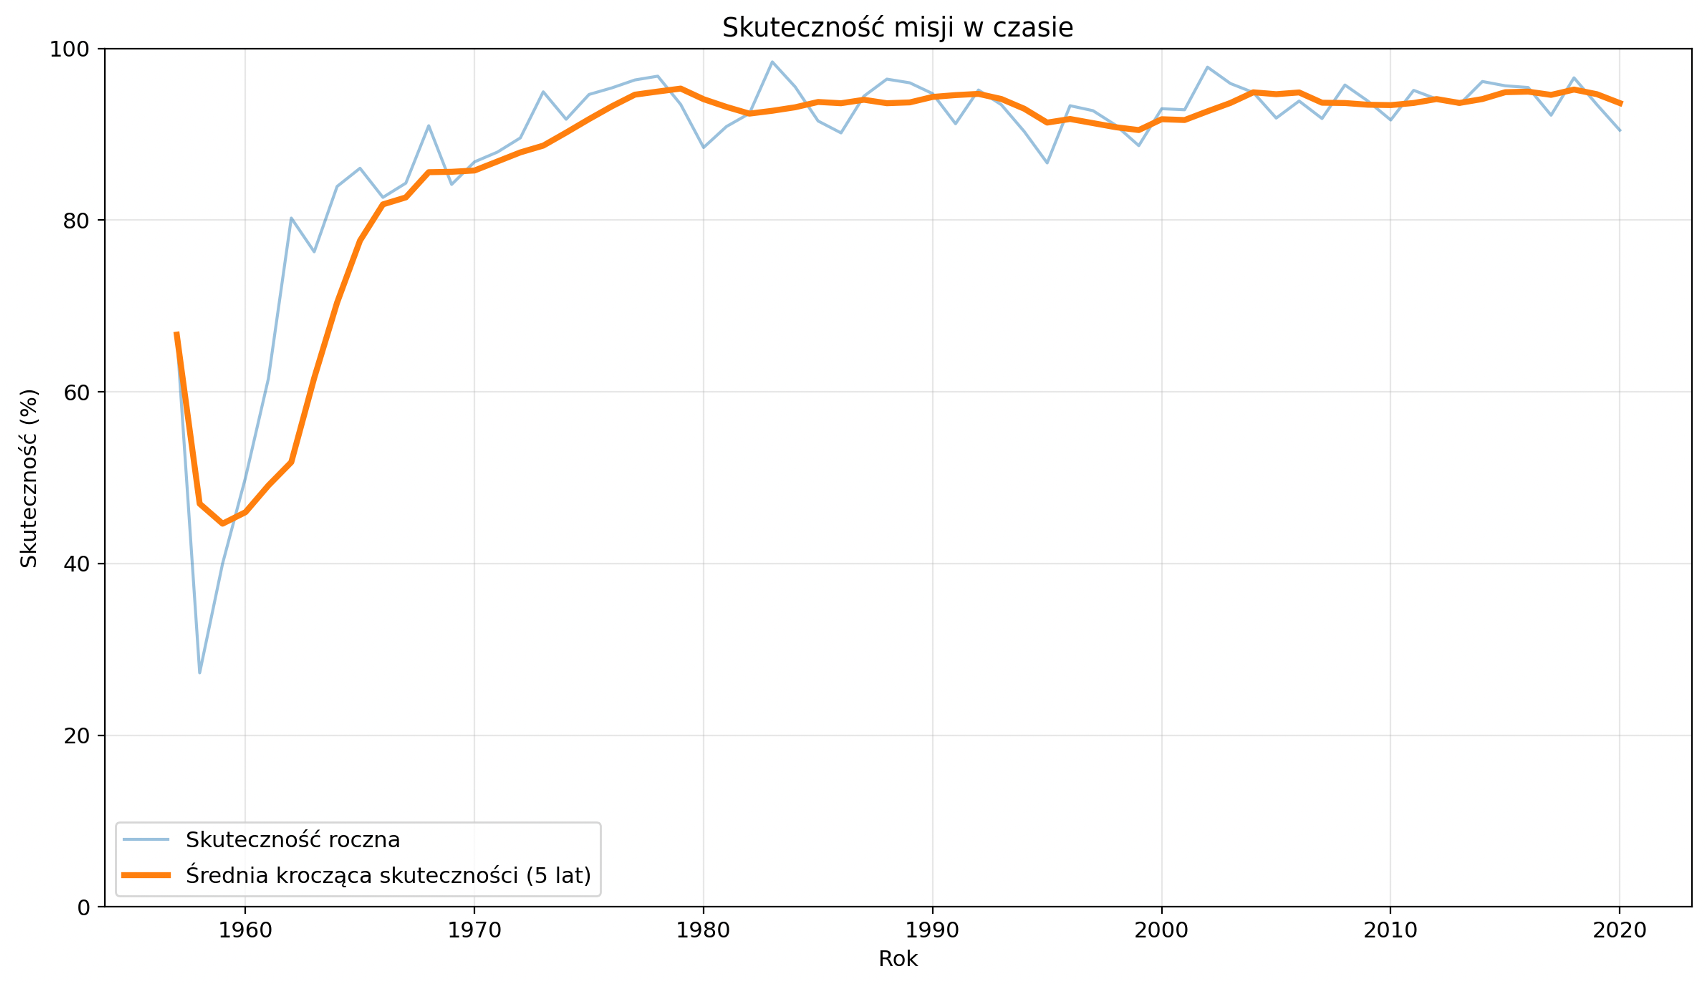
\includegraphics[width=\textwidth]{phts/5/png/5.8.png}
    \caption{Skuteczność misji kosmicznych w czasie.}
\end{figure}

Wykres przedstawia roczną skuteczność misji oraz pięcioletnią średnią kroczącą.
Na początku ery kosmicznej skuteczność była znacznie bardziej niestabilna, co jest naturalne dla okresu intensywnych eksperymentów i rozwoju nowych technologii.
W późniejszych latach skuteczność ustabilizowała się na wysokim poziomie.

Od lat 70. skuteczność misji najczęściej oscyluje w okolicach 90\% lub więcej.
Pokazuje to duży postęp technologiczny oraz coraz większą przewidywalność i dojrzałość systemów wykorzystywanych w lotach kosmicznych.


\subsubsection{Skuteczność misji kosmicznych według dekad}
\begin{figure}[H]
    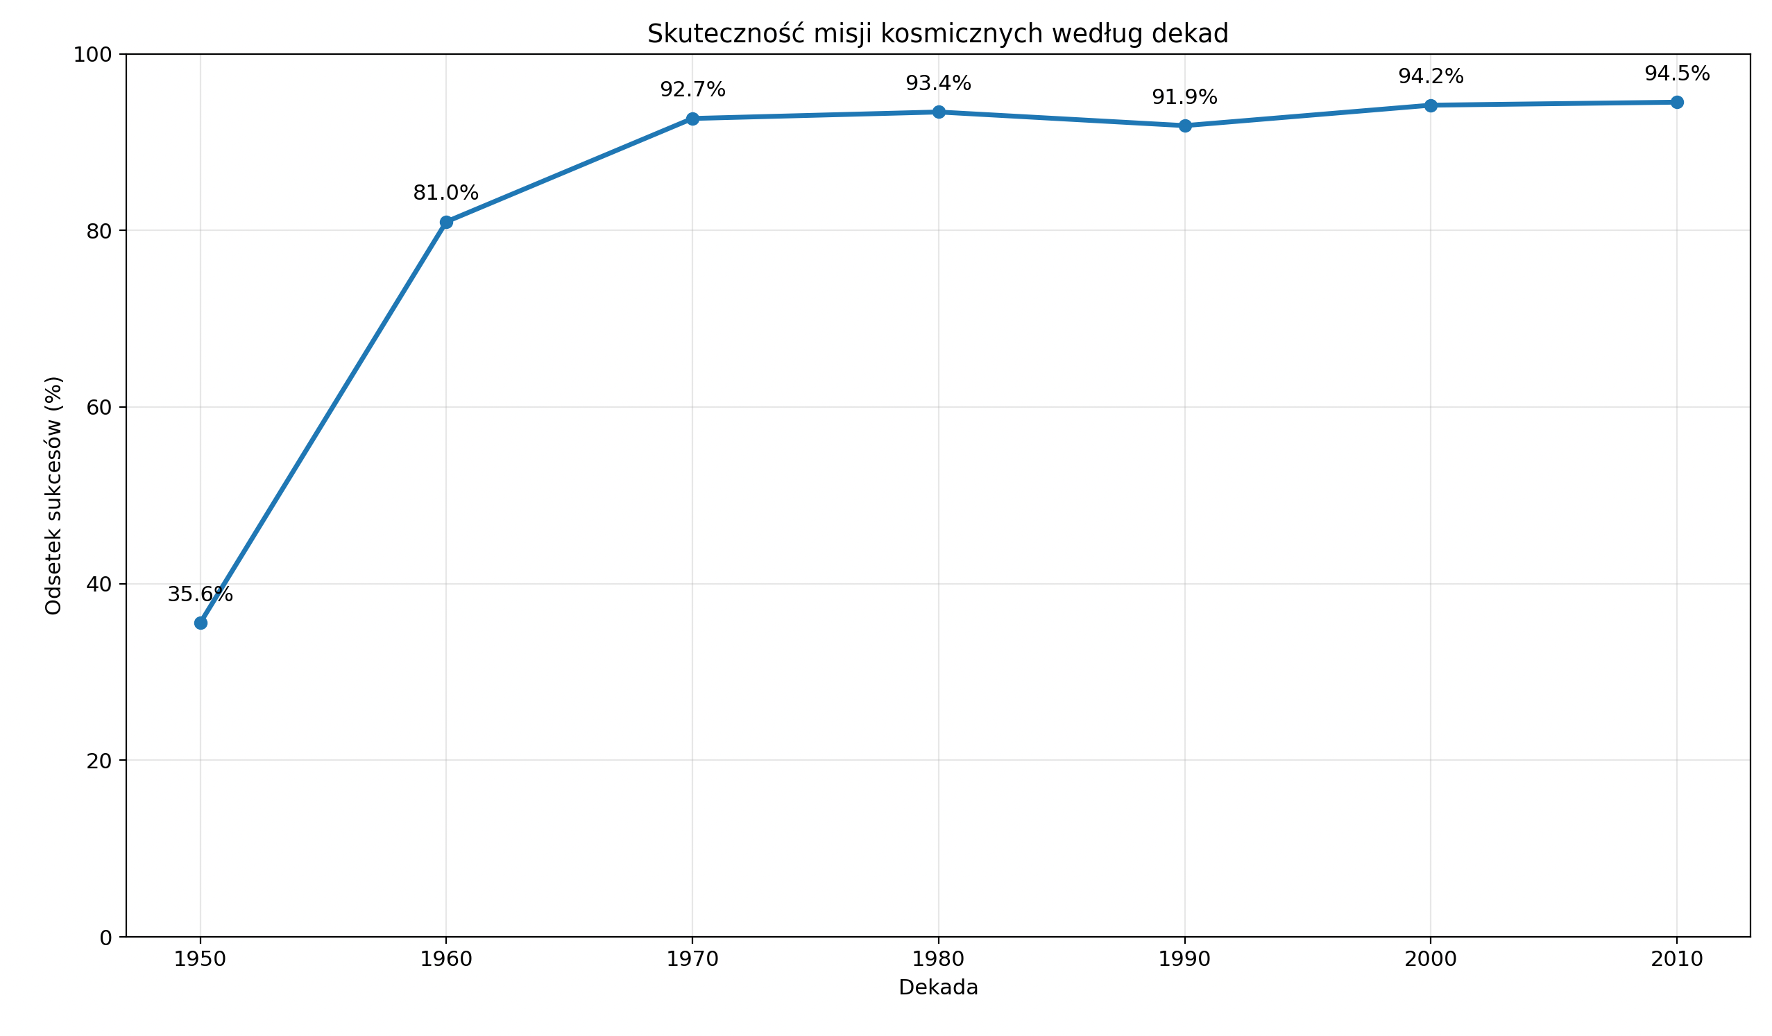
\includegraphics[width=\textwidth]{phts/5/png/5.9.png}
    \caption{Skuteczność misji kosmicznych według dekad.}
\end{figure}

Wykres pokazuje skuteczność misji kosmicznych w kolejnych dekadach.
W latach 50. skuteczność wynosiła jedynie 35.6\%, co dobrze pokazuje eksperymentalny charakter pierwszych misji kosmicznych.
Już w latach 60. skuteczność wzrosła jednak do 81.0\%.

Od lat 70. skuteczność utrzymuje się na bardzo wysokim poziomie, najczęściej powyżej 90\%.
Najwyższa wartość widoczna jest dla lat 2010., gdzie skuteczność wynosi 94.5\%.
Oznacza to, że wraz z rozwojem technologii i doświadczenia operacyjnego ryzyko niepowodzenia misji znacząco się zmniejszyło.


\subsubsection{Skuteczność misji w top 10 krajów}
\begin{figure}[H]
    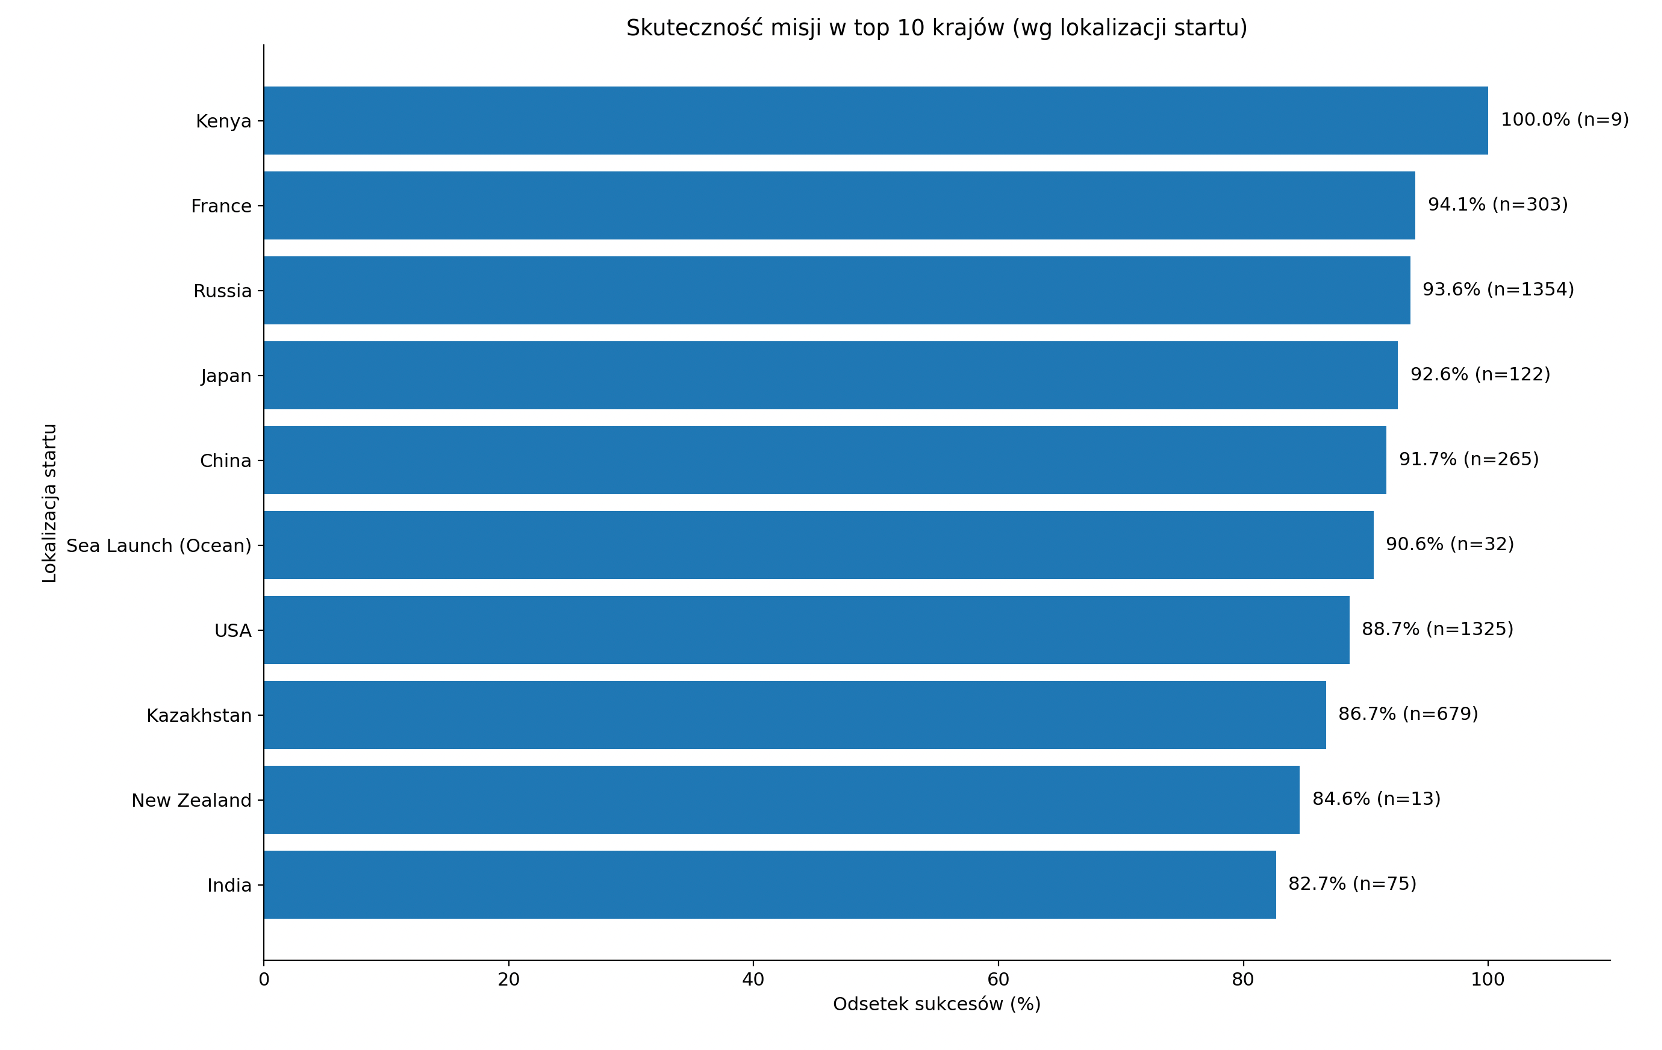
\includegraphics[width=\textwidth]{phts/5/png/5.10.png}
    \caption{Skuteczność misji w top 10 krajów według lokalizacji startu.}
\end{figure}

Wykres przedstawia skuteczność misji dla dziesięciu najważniejszych lokalizacji startu.
Najwyższą skuteczność osiąga Kenia, gdzie wszystkie 9 misji zakończyło się sukcesem.
Należy jednak pamiętać, że w tym przypadku liczba misji jest bardzo mała, więc wynik 100\% trzeba interpretować ostrożnie.

Wśród krajów z dużą liczbą misji bardzo wysoką skuteczność osiągają Francja, Rosja, Japonia oraz Chiny.
Rosja i USA mają bardzo duże liczby misji, a jednocześnie utrzymują skuteczność na poziomie odpowiednio około 93.6\% i 88.7\%.
Pokazuje to, że duża skala aktywności nie musi oznaczać niskiej skuteczności.


\subsubsection{Koszt misji kosmicznych w czasie}
\begin{figure}[H]
    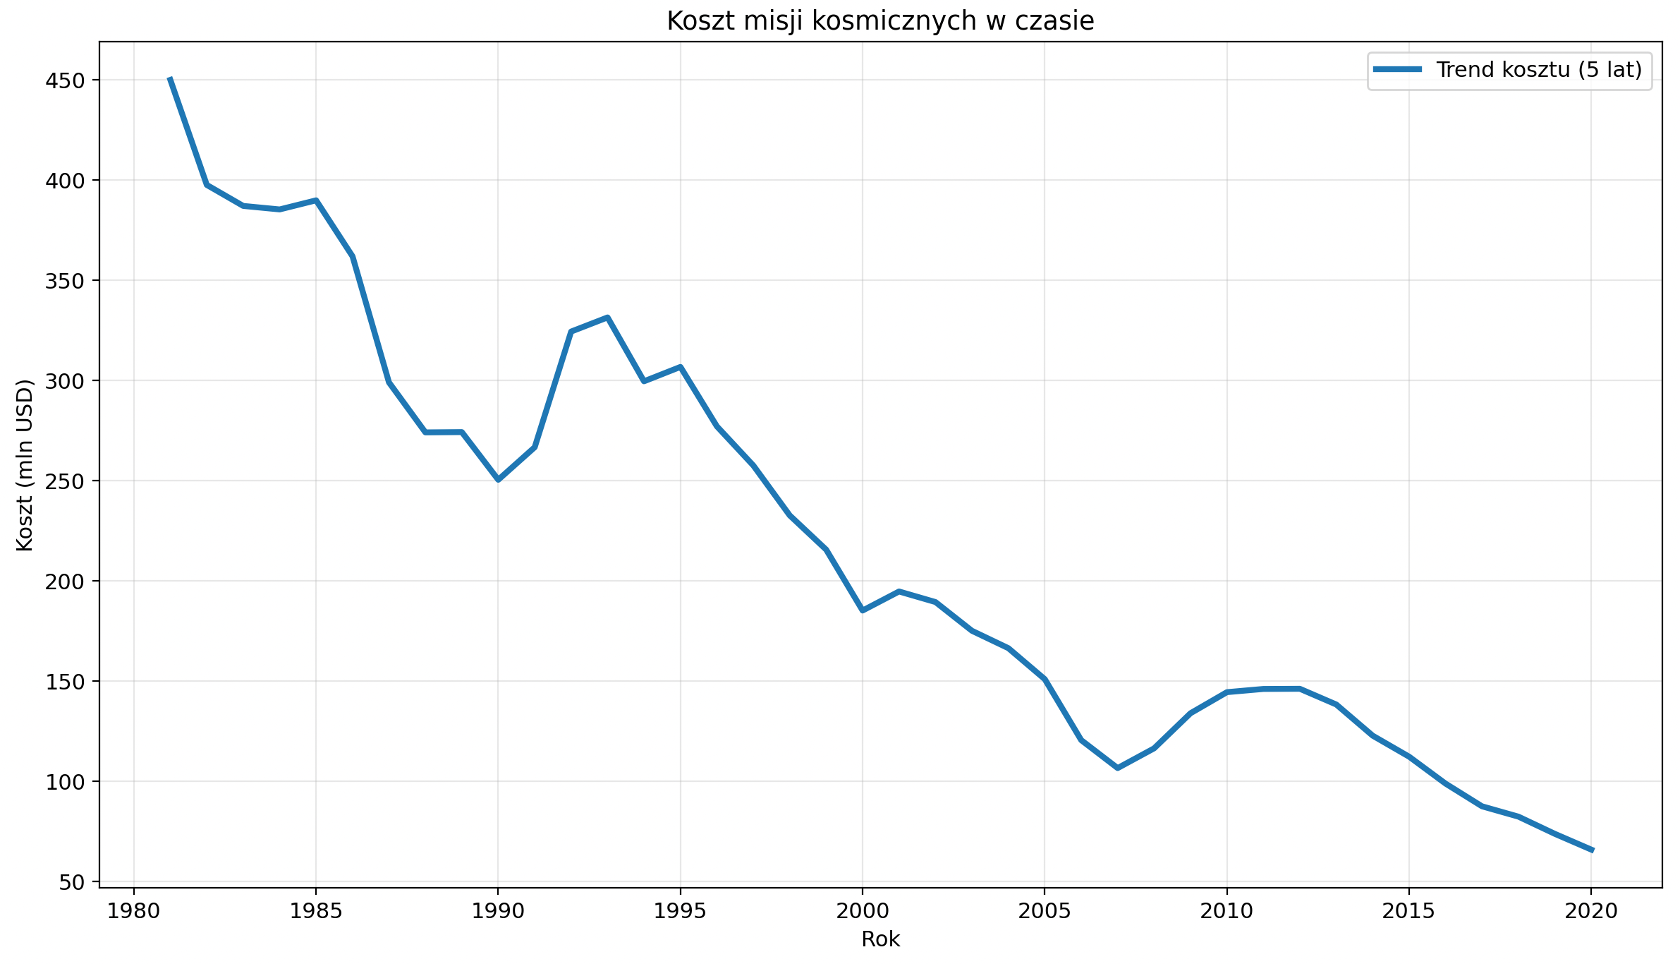
\includegraphics[width=\textwidth]{phts/5/png/5.11.png}
    \caption{Koszt misji kosmicznych w czasie.}
\end{figure}

Wykres przedstawia pięcioletni trend kosztu misji kosmicznych w milionach dolarów.
Widoczna jest ogólna tendencja spadkowa - od wartości przekraczających 400 mln USD na początku analizowanego okresu kosztowego do znacznie niższych wartości w latach 2010.
Sugeruje to, że wraz z rozwojem technologii i zwiększeniem doświadczenia operacyjnego koszty misji stopniowo malały.

Trzeba jednak pamiętać, że dane kosztowe są dostępne tylko dla części misji.
W związku z tym wykres nie opisuje wszystkich startów kosmicznych, lecz jedynie te, dla których w zbiorze podano informację o koszcie.


\subsection{Wnioski}
\begin{enumerate}
    \item Największa liczba misji kosmicznych przypadła na lata 60. i 70., czyli okres intensywnej rywalizacji kosmicznej.
    \item Najwięcej startów przeprowadzono z Rosji oraz Stanów Zjednoczonych, które zdecydowanie dominują pod względem liczby misji.
    \item Najaktywniejszą organizacją w całym zbiorze było RVSN USSR, znacznie przewyższające pozostałe firmy i agencje.
    \item Skuteczność misji kosmicznych wzrosła z 35.6\% w latach 50. do ponad 90\% w kolejnych dekadach.
    \item Większość misji zakończyła się sukcesem - 3794 przypadki, czyli około 90.38\% całego zbioru.
    \item W ostatnich latach widoczny jest ponowny wzrost liczby misji, co może wskazywać na rozwój sektora prywatnego i wzrost znaczenia nowych państw w eksploracji kosmosu.
    \item Koszt misji kosmicznych w czasie wykazuje ogólną tendencję spadkową, jednak analiza kosztów dotyczy tylko części obserwacji.
\end{enumerate}

\newpage
\section{Studenci wg płci oraz podgrup kierunków (Python)}

Przygotowane przez: Maciej Kurzydłowski

\subsection{Źródło danych}
\href{https://bdl.stat.gov.pl/bdl/metadane/cechy/3566?back=True}
{Studenci i absolwenci wg form własności uczelni, form studiów, płci, oraz podgrup kierunków studiów klasyfikacji ISCED-F 2013} \\
\url{https://bdl.stat.gov.pl/bdl/metadane/cechy/3566?back=True}

\subsection{Opis zbioru i istotnych pojęć}
\begin{itemize}
    \item Do 2016 r. dane pozyskiwane są ze sprawozdawczości GUS. Od 2017 r. dane opracowano na podstawie systemu POL-on administrowanego przez Ministerstwo Edukacji i Nauki.
    \item Dane nie obejmują uczelni prowadzonych przez kościoły oraz szkół resortu obrony narodowej i resortów spraw wewnętrznych.
    \item Zbiór zawiera liczbę studentów i absolwentów z podziałem na: formę własności uczelni (publiczne / niepubliczne), formę studiów (stacjonarne / niestacjonarne), płeć oraz podgrupy kierunków według klasyfikacji ISCED‑F 2013.
    \item Zbiór zawiera dane z lat 2014-2024, z ostatnią aktualizacją 23/10/2025.
\end{itemize}

\subsection{Wizualizacje zbioru}

\subsubsection{Liczba studentów w Polsce}
\begin{figure}[H]
    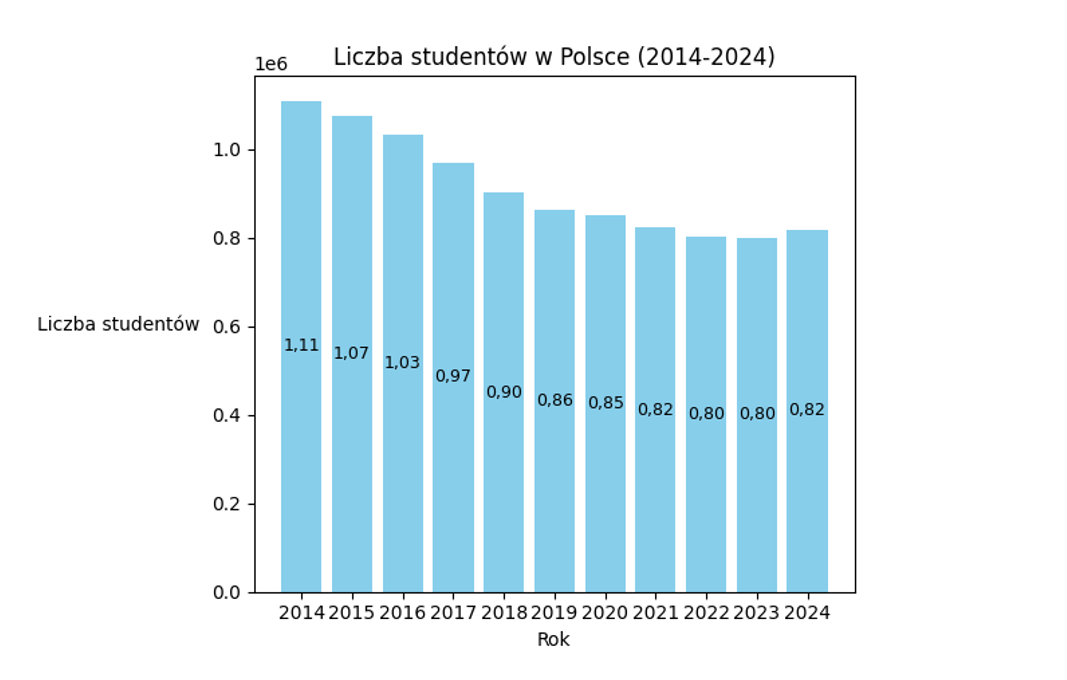
\includegraphics[width=\textwidth]{phts/6/png/6.1.png}
    \caption{Liczba studentów w Polsce (2014-2024).}
\end{figure}

\begin{figure}[H]
    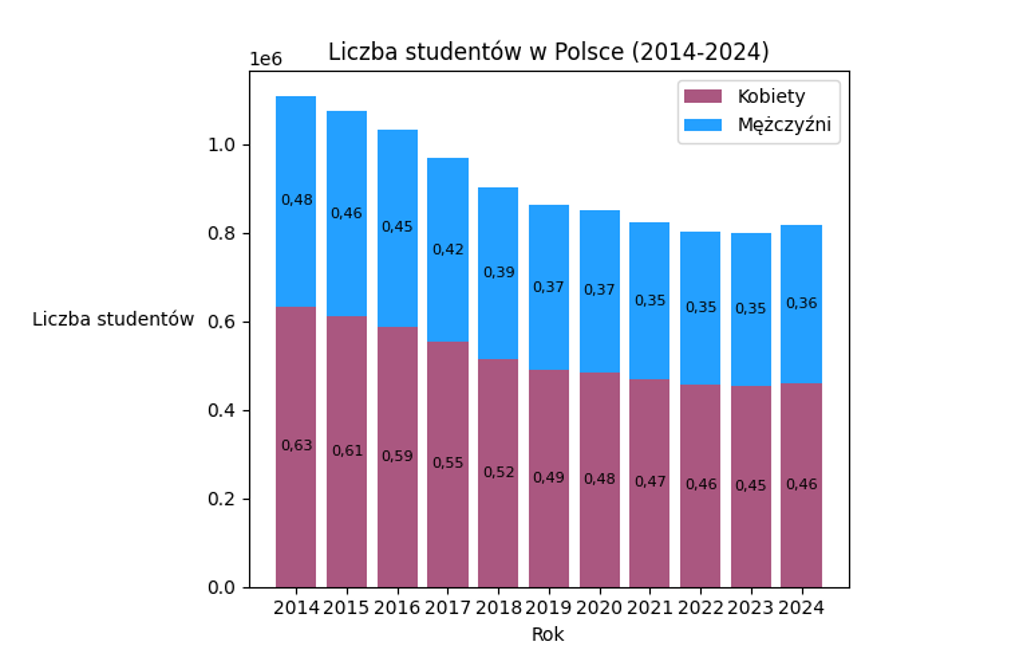
\includegraphics[width=\textwidth]{phts/6/png/6.2.png}
    \caption{Liczba studentów w Polsce według płci (2014-2024).}
\end{figure}

W latach 2014-2024 liczba studentów zmniejszyła się z około 1.1 miliona do około 0.8 miliona, co oznacza spadek o około 27\%.
Stosunek kobiet do mężczyzn nie zmienił się znacząco, utrzymując się na poziomie około 60\% kobiet i 40\% mężczyzn. 
Spadek liczby studentó jest prawdopodobnie związany z ogólnym trendem demograficznym w Polsce, gdzie liczba osób w wieku studenckim maleje.


\subsubsection{Najpopularniejsze kierunki studiów}
\begin{figure}[H]
    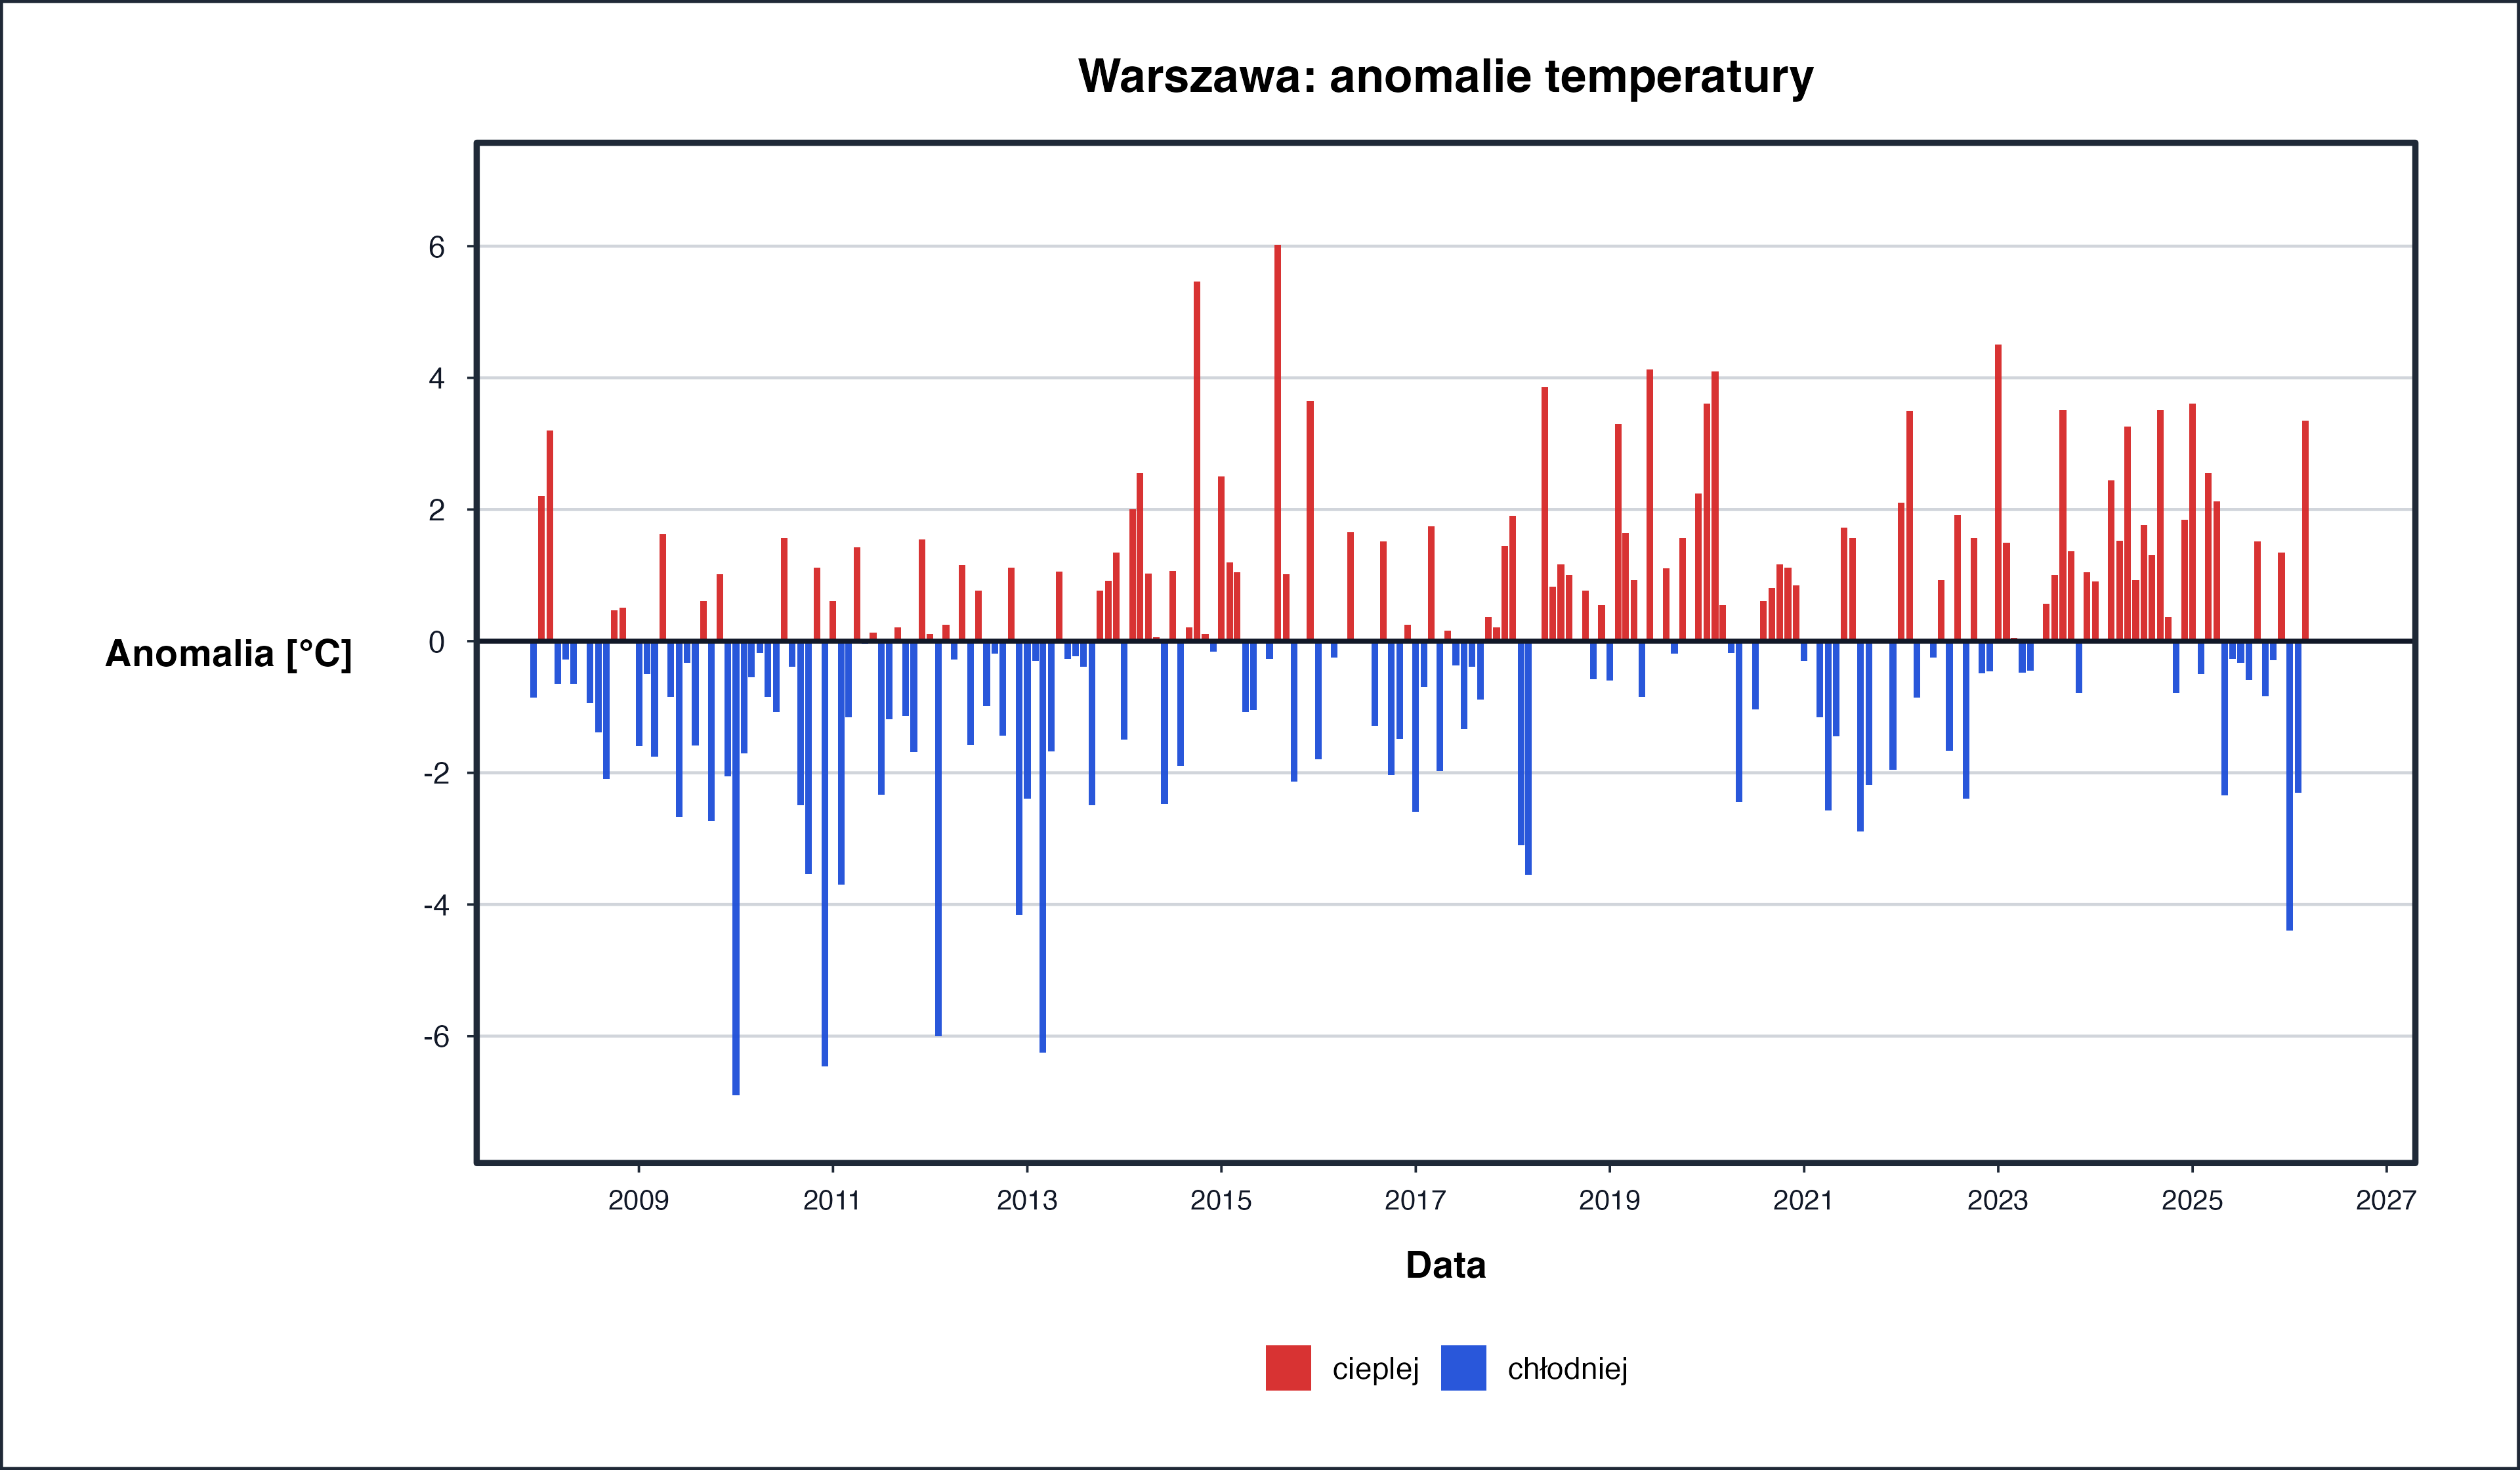
\includegraphics[width=\textwidth]{phts/6/png/6.3.png}
    \caption{Najpopularniejsze kierunki studiów (2014).}
\end{figure}

\begin{figure}[H]
    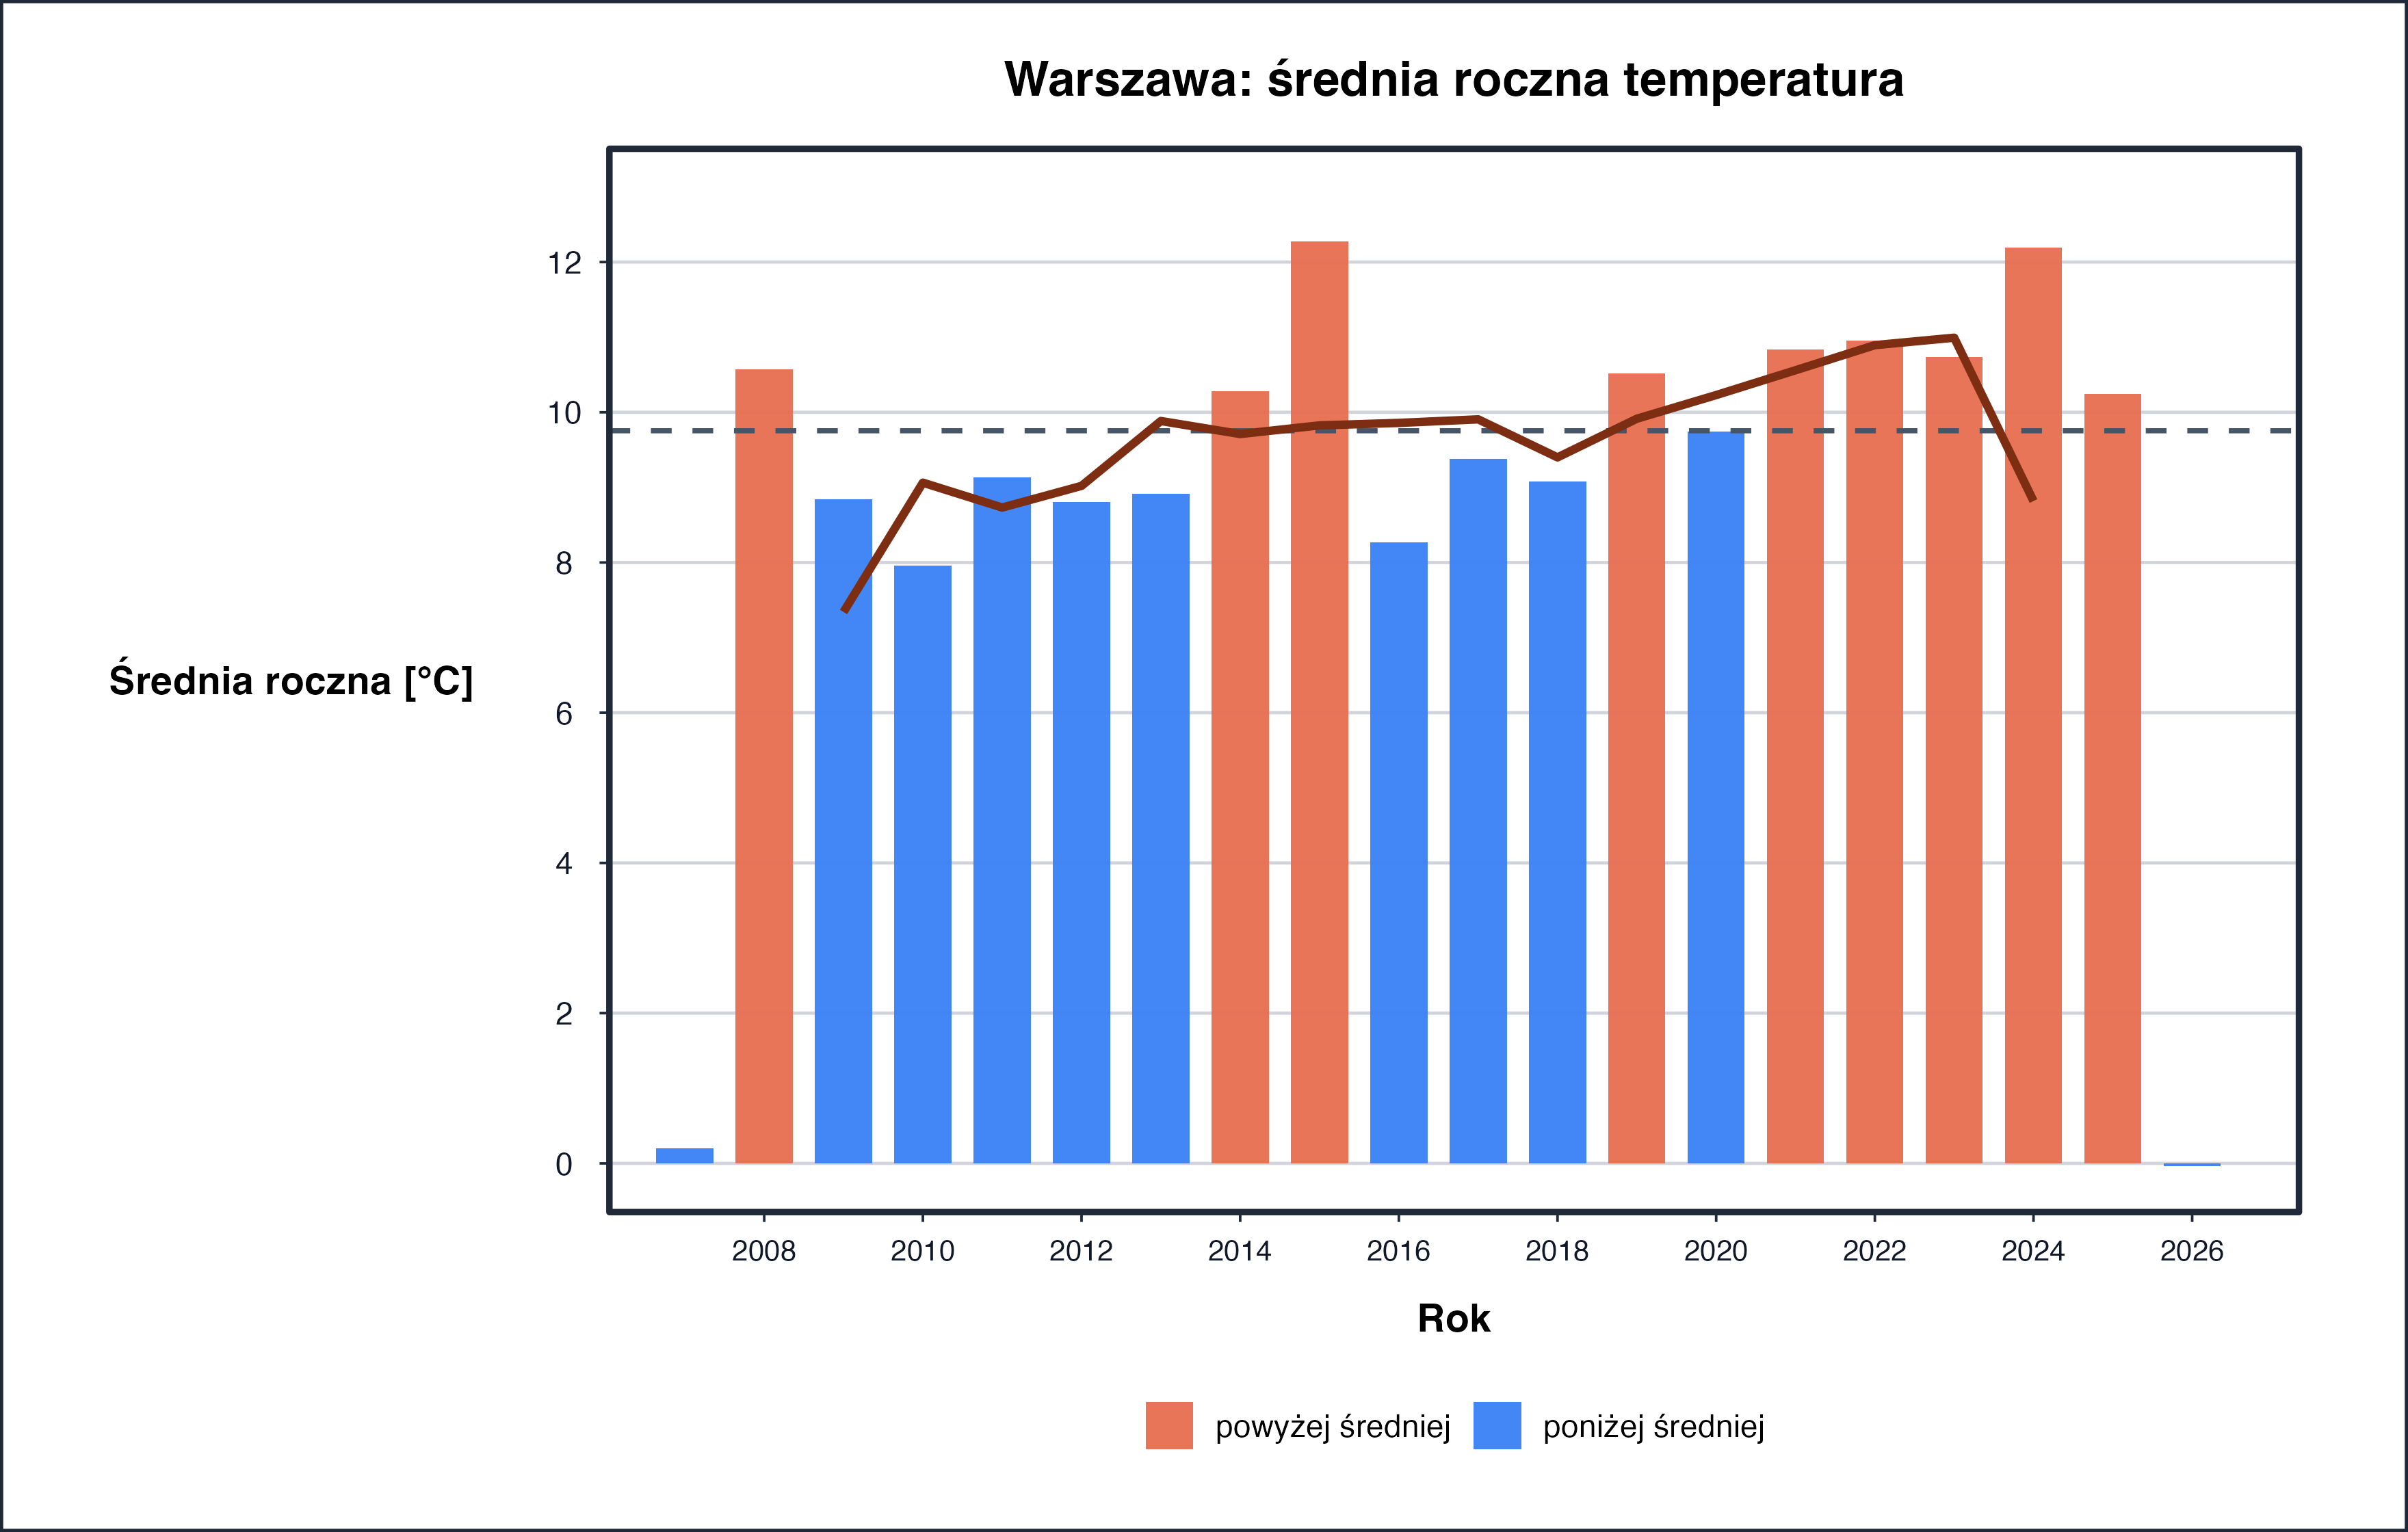
\includegraphics[width=\textwidth]{phts/6/png/6.4.png}
    \caption{Najpopularniejsze kierunki studiów (2024).}
\end{figure}

W 2014 dominowały kierunki biznesowe i inżynieryjne, natomiast w 2024 najpopularniejszym stał się kierunek medyczny.
Kierunki językowe i społeczne zyskały na znaczeniu, a niektóre kierunki, takie jak produkcja i przetwórstwo oraz pedagogika, straciły na popularności.
Technologie telekomunikacyjne jako kierunek studiów, nie zmienił się na przestrzeni dekady, utrzymując się na podobnym poziomie popularności.

Zmiany te sugerują zmianę preferencji edukacyjnych, w obszary ścisłe i medyczne, co jest zgodne z globalnymi trendami na rynku pracy, gdzie rośnie zapotrzebowanie na specjalistów w tych dziedzinach.


\subsubsection{Najmniej popularne kierunki studiów}
\begin{figure}[H]
    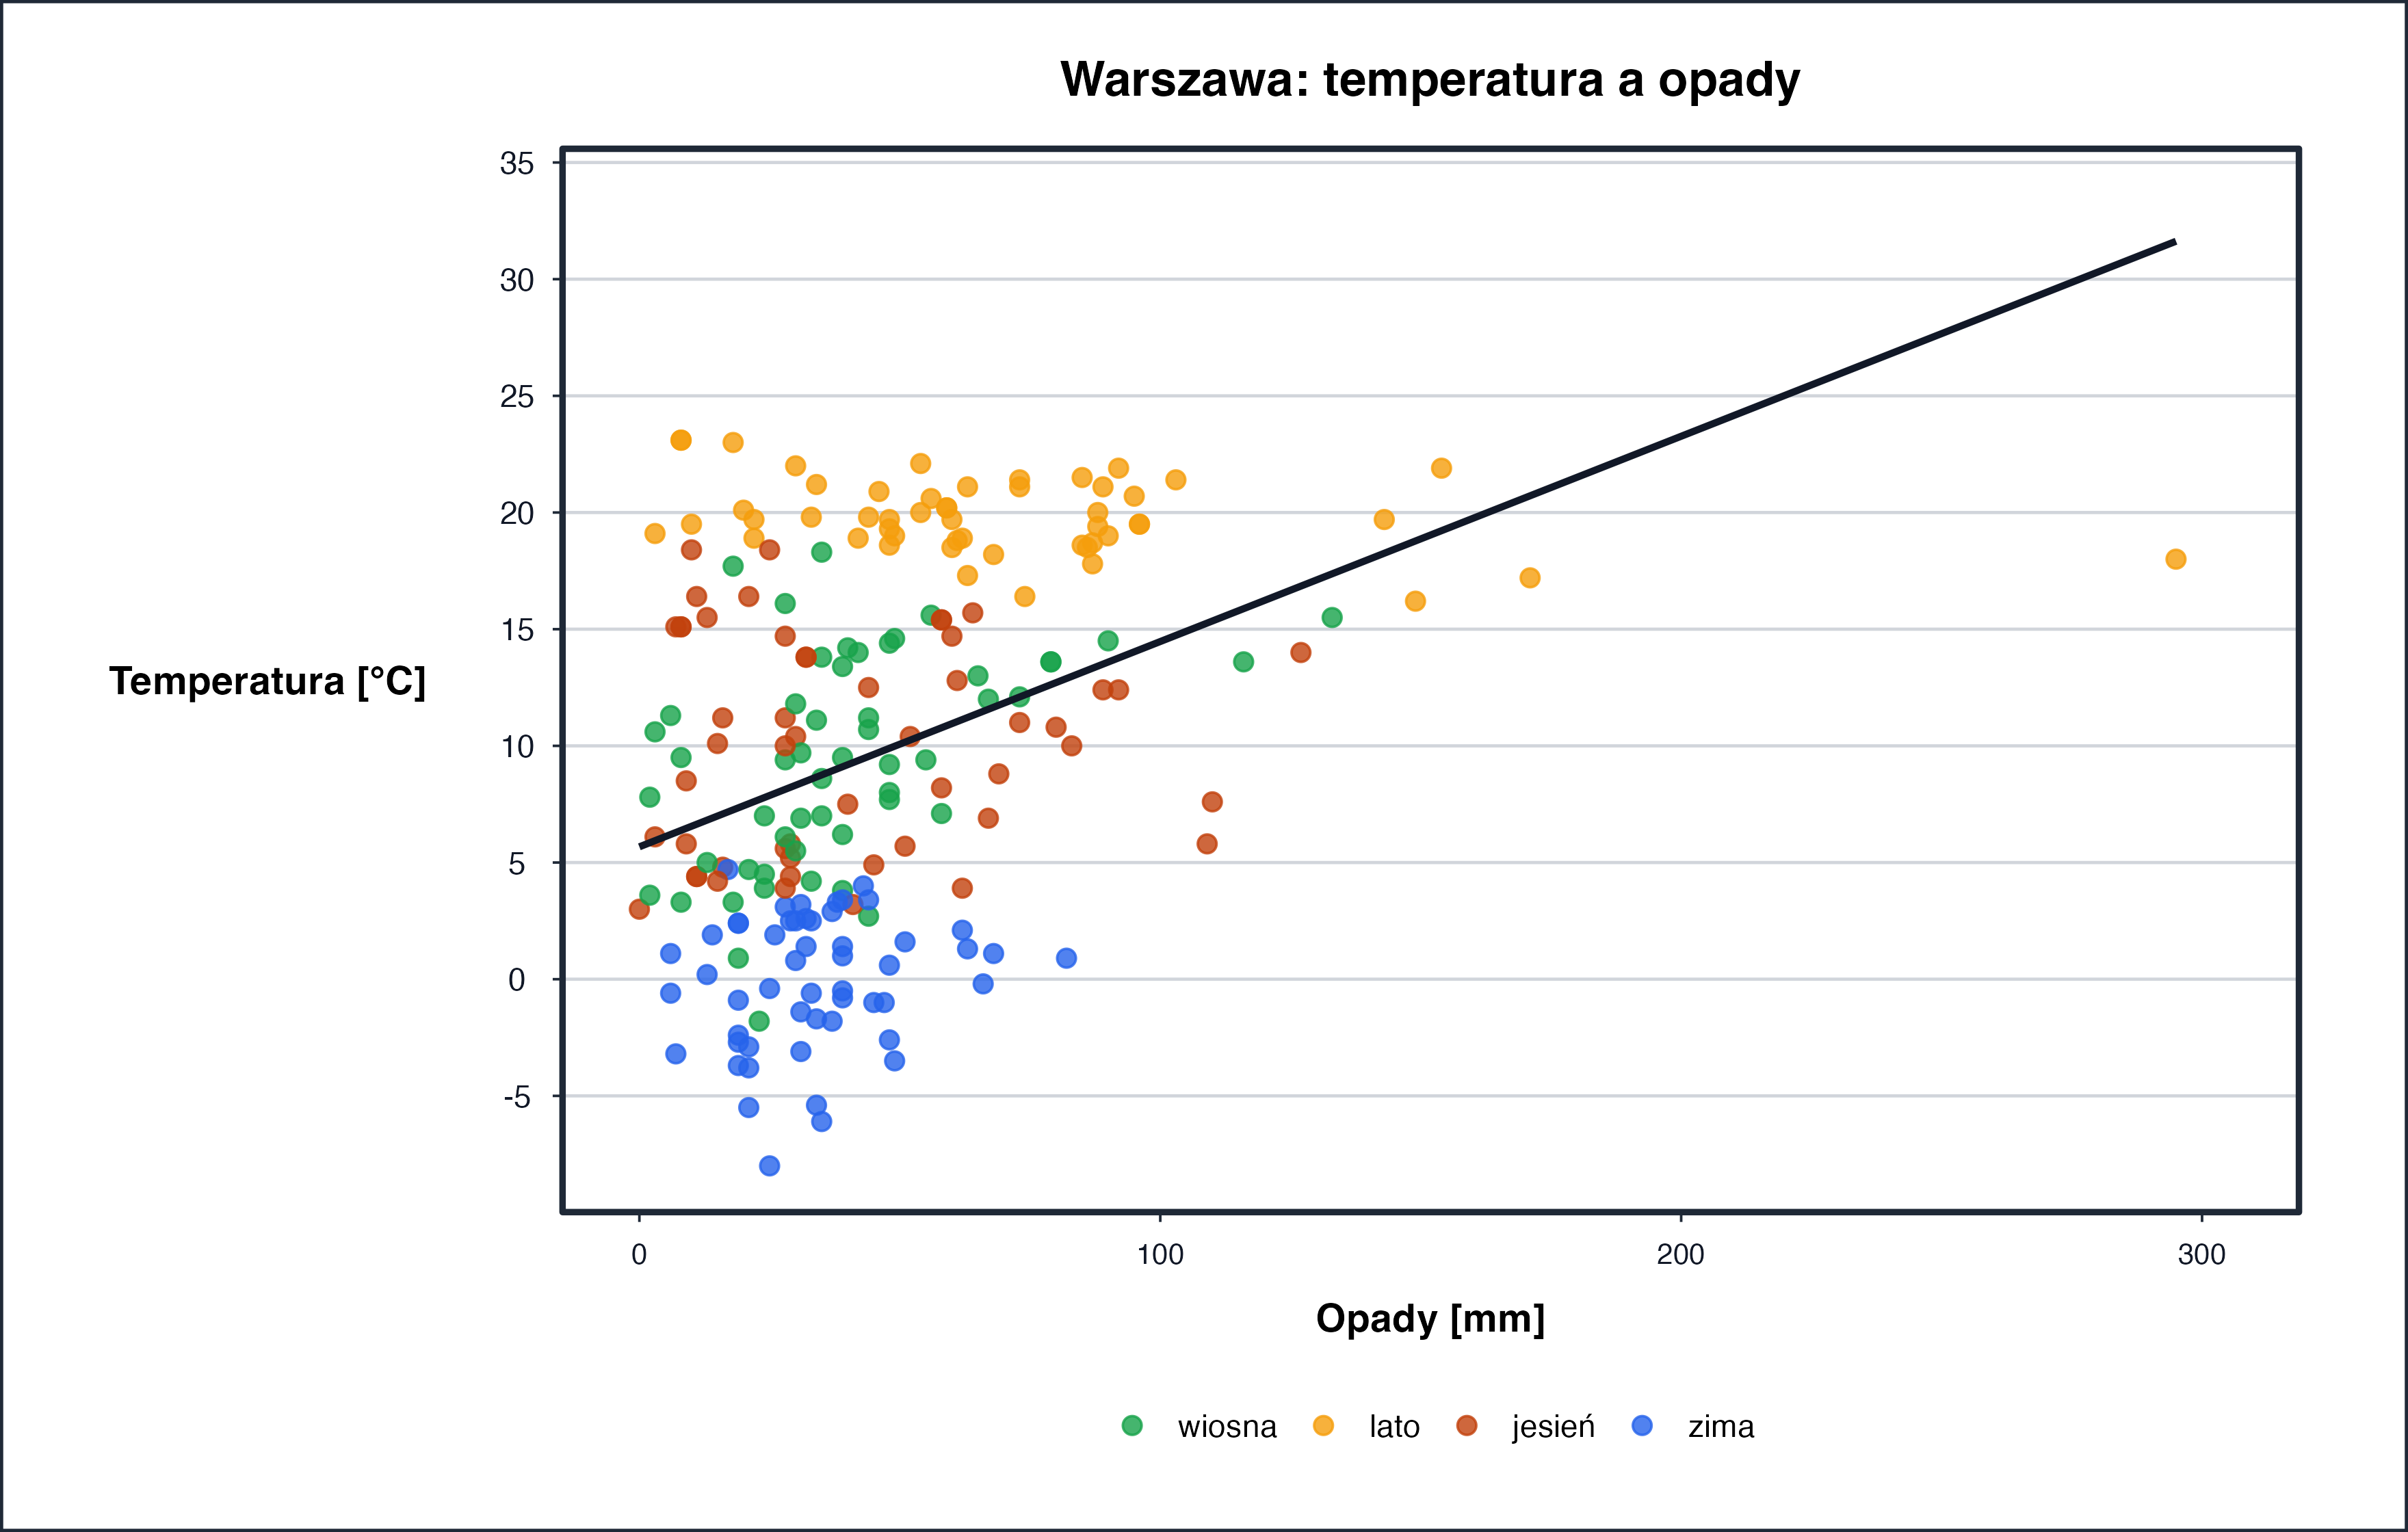
\includegraphics[width=\textwidth]{phts/6/png/6.5.png}
    \caption{Najmniej popularne kierunki studiów (2014).}
\end{figure}

\begin{figure}[H]
    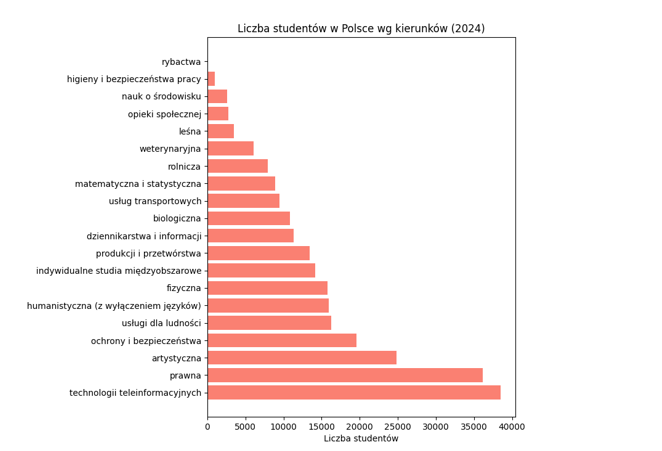
\includegraphics[width=\textwidth]{phts/6/png/6.6.png}
    \caption{Najmniej popularne kierunki studiów (2024).}
\end{figure}

Najmniej popularne kierunki: rybactwo i higiena i bezpieczeństwo pracy, nie zmieniły się znacząco w ciągu dekady, utrzymując się na bardzo niskim poziomie liczby studentów.
Kierunek nauk o środwisku stracił znacząco na popularności, co jest najprawdopodobniej związane z brakiem zainteresowania tym obszarem wśród młodych ludzi, mimo rosnącej świadomości ekologicznej.
Weterynaryjny kierunek studiów zyskał na popularności, co może być związane z rosnącym zainteresowaniem opieką nad zwierzętami.


\subsubsection{Studenci w województwach}
\begin{figure}[H]
    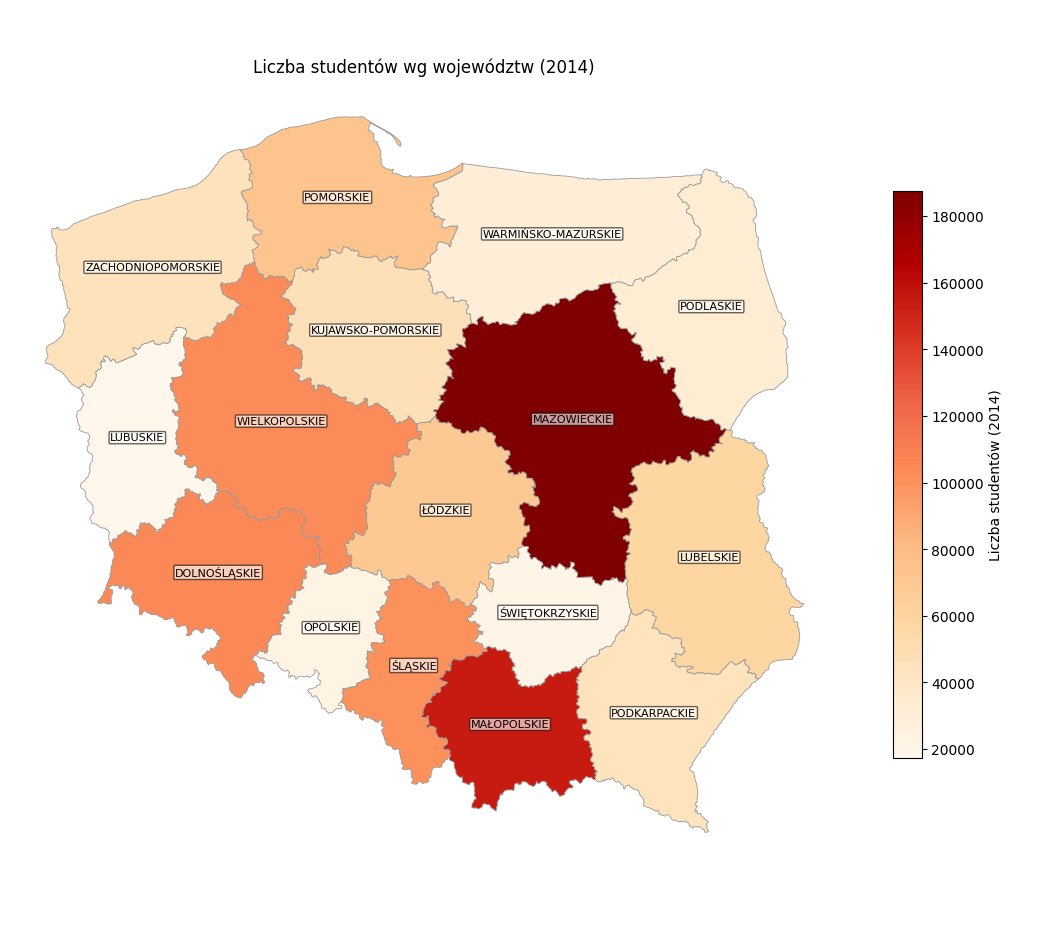
\includegraphics[width=\textwidth]{phts/6/png/6.7.png}
    \caption{Liczba studentów w województwach (2014).}
\end{figure}

Mapy pokazują silną koncentracje studentów w województwach: mazowieckim, małopolskim oraz dolnośląskim. Co spowodowane jest obecnością największych ośrodków akademickich, takich jak Warszawa, Kraków i Wrocław.


\begin{figure}[H]
    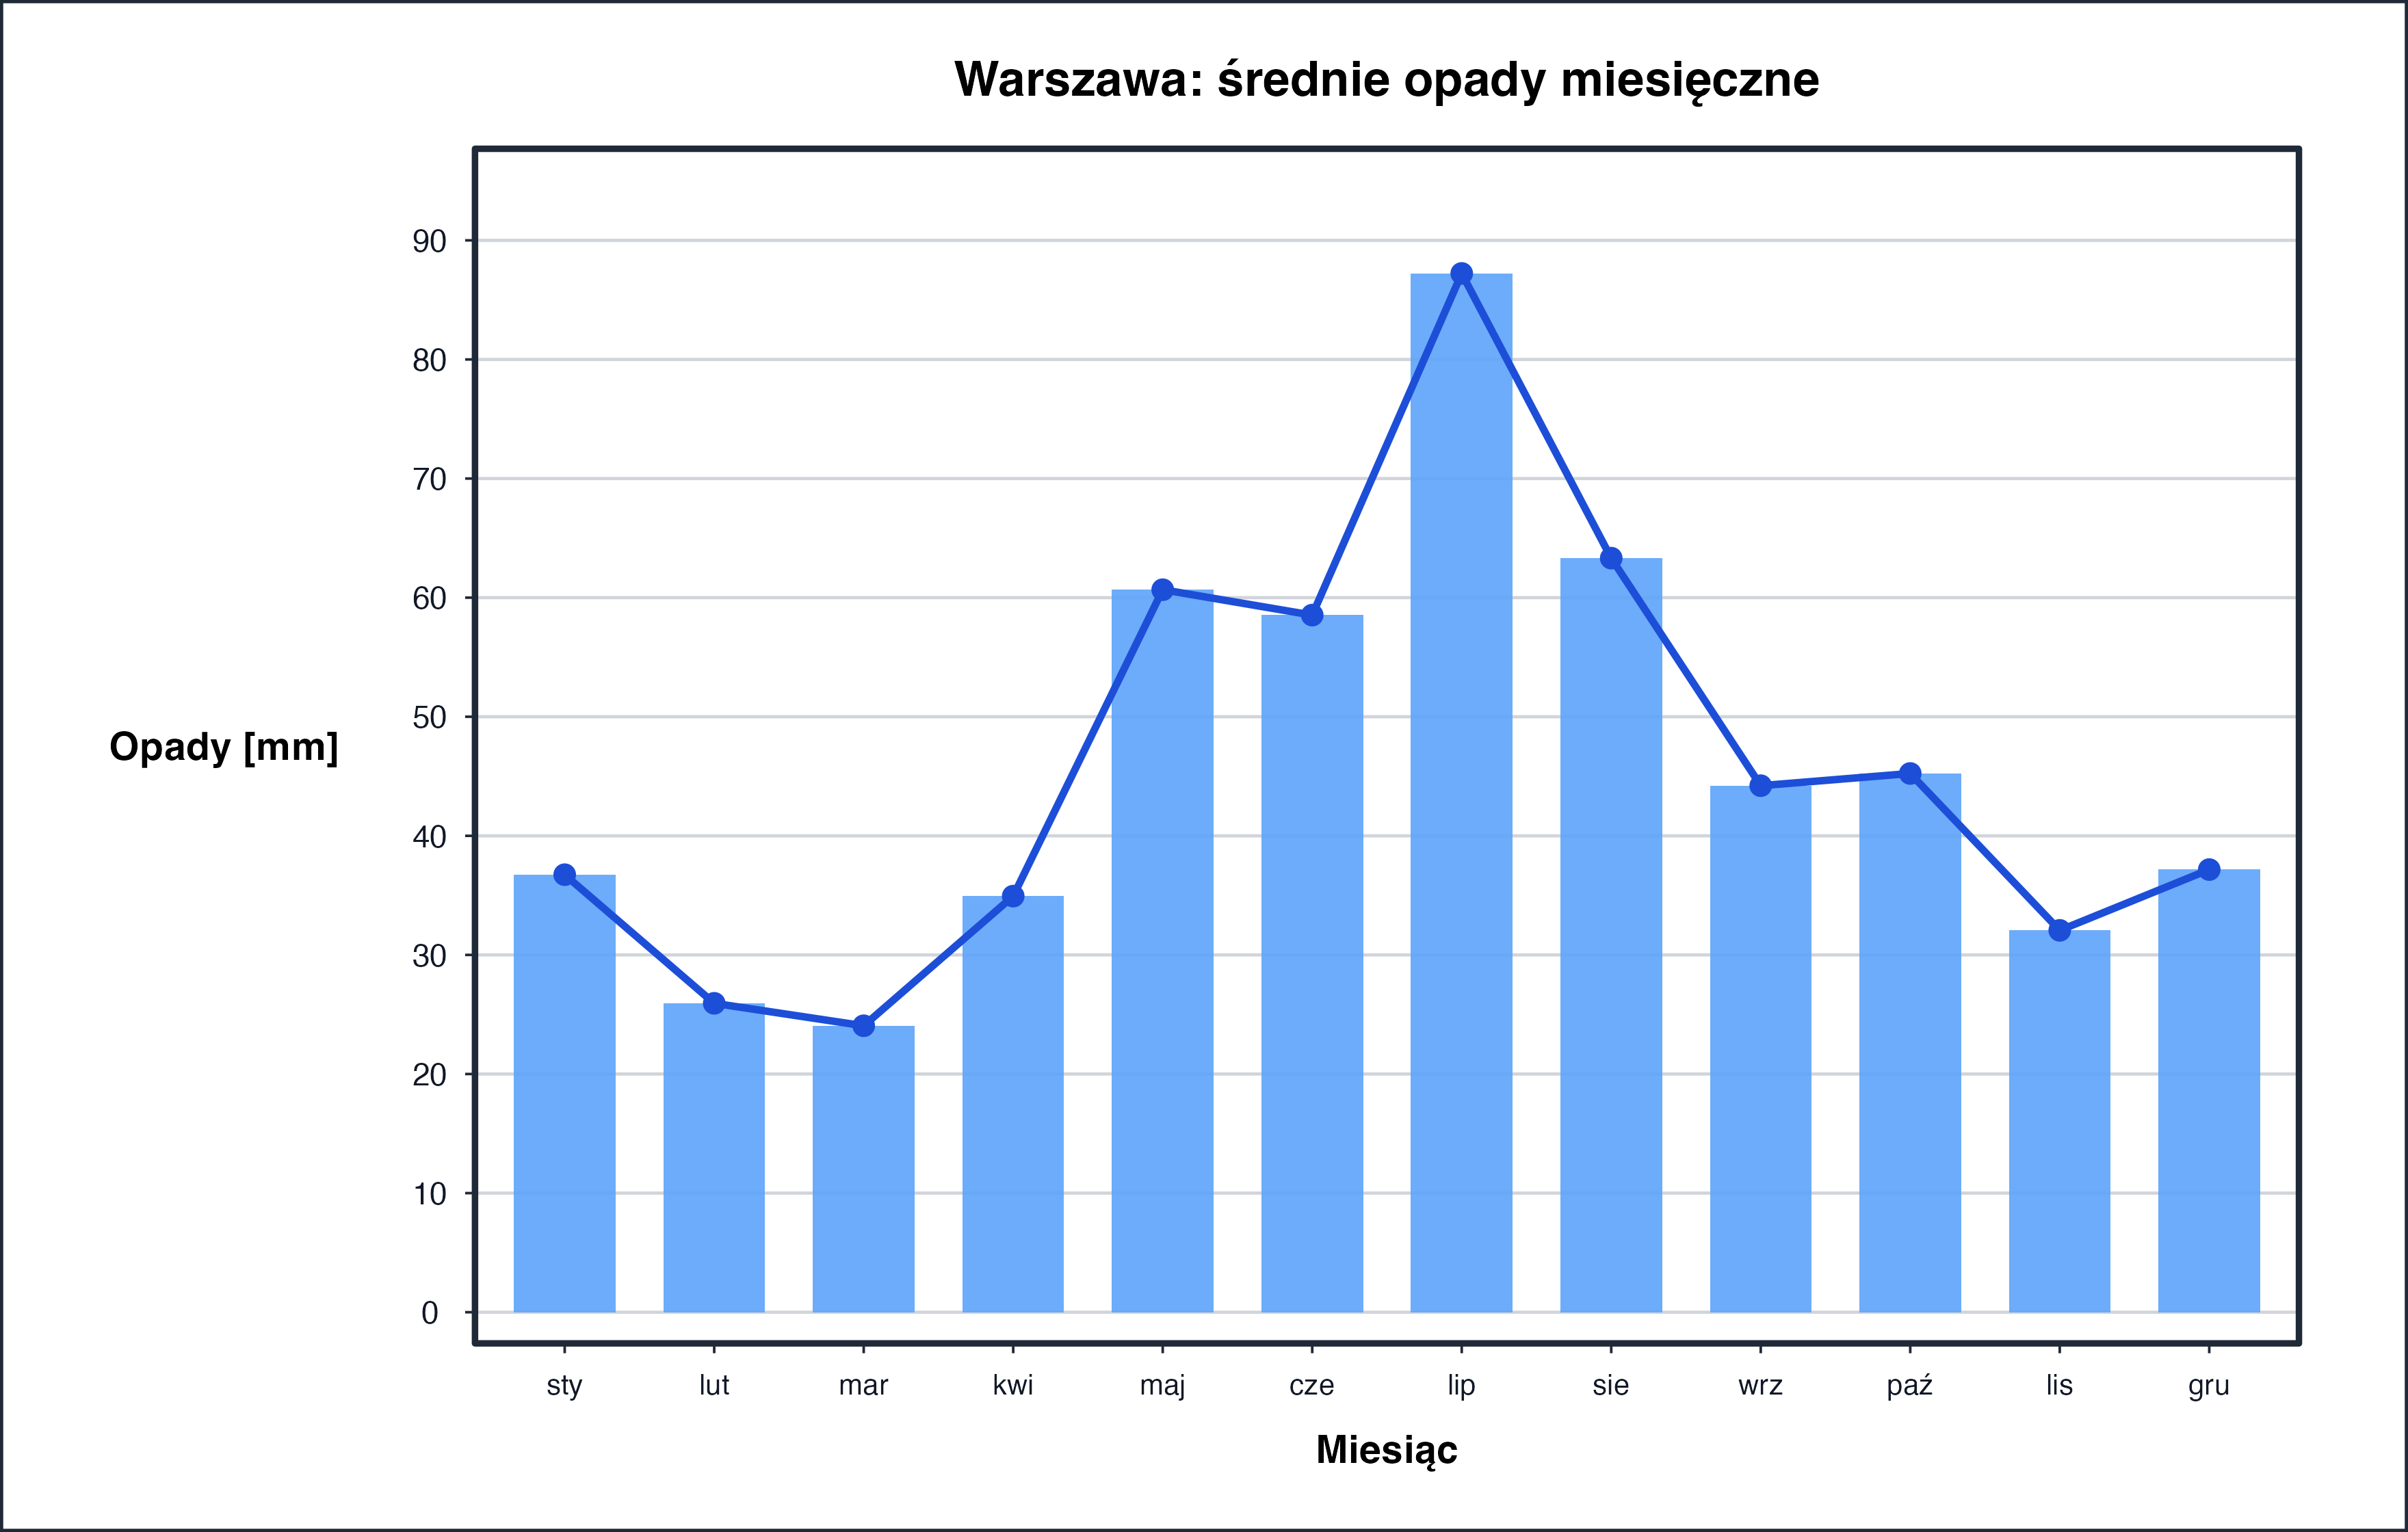
\includegraphics[width=\textwidth]{phts/6/png/6.8.png}
    \caption{Liczba studentów w województwach (2024).}
\end{figure}

W porównaniu 2024 z 2014 rokiem, liczba studentów nie zmieniła wystarczająco aby zaobserwować znaczące zmiany w rozkładzie geograficznym wraz z dominacją uczelni warszawskich.


\newpage

\subsubsection{Kierunek w stosunku do województw}

\begin{figure}[H]
    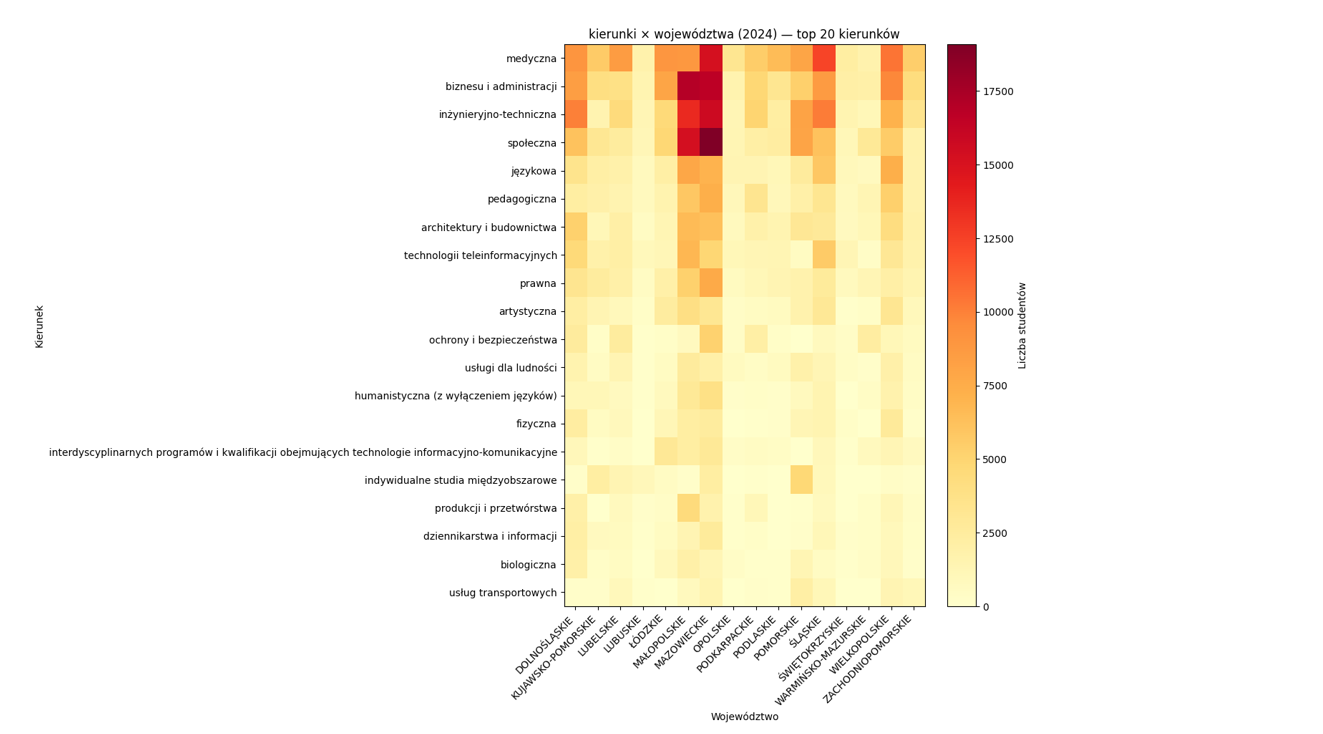
\includegraphics[width=\textwidth]{phts/6/png/6.9.png}
    \caption{Liczba studentów w województwach według kierunków studiów (2024).}
\end{figure}

Wykres pokazuje silną koncentracje w województwach: mazowieckim oraz małopolskim, gdzie dominują kierunki: medycyna, biznes i administracja, inżynieryjno-techniczna, społeczny.
W pozostałych województwach zauważalna jest tendencja do tych samych kierunków, jednak nie jest ona tak silna jak w przypadku mazowieckiego i małopolskiego.

Kierunek produkcja i przetwórstwo jest najbardziej popularny w województwie małopolskim, z znaczącą przewagą nad innymi regionami, co czyni to województwo małopolskie liderem w tej kategorii.

\subsection{Wnioski}
\begin{enumerate}
    \item Liczba studentów w Polsce spadła o około 27\% w latach 2014-2024, co jest prawdopodobnie związane z ogólnym trendem demograficznym.
    \item Stosunek kobiet do mężczyzn wśród studentów utrzymuje się na poziomie około 60\% kobiet i 40\% mężczyzn.
    \item Najpopularniejszym kierunkiem studiów w 2014 roku jest biznes i administracja, a najmniej popularne to rybactwo i higiena i bezpieczeństwo pracy.
    \item Najpopularniejszym kierunkiem studiów w 2024 roku jest medycyna, gdzie najmniej popularne kierunki nie zmieniły się od 2014 roku.
    \item Największa koncentracja studentów znajduje się w województwach mazowieckim, małopolskim oraz dolnośląskim, co jest związane z obecnością największych ośrodków akademickich.
    \item Kierunki studiów takie jak medycyna, biznes i administracja, inżynieryjno-techniczna oraz społeczny są dominujące w województwach mazowieckim i małopolskim.
\end{enumerate}

\newpage

\section{Temperatura i opady w wybranych miastach Europy (R)}

Przygotowane przez: Jan Domański, Maciej Kurzydłowski

\subsection{Źródło danych}
Dane wykorzystane w tej części projektu pochodzą z czterech plików CSV przygotowanych dla wybranych miast europejskich: Warszawy, Paryża, Dublina oraz Lizbony.

Pliki zostały uzyskane przez scraper ze strony \url{https://www.ogimet.com/gclimat.phtml.en}.

\begin{itemize}
    \item \texttt{warsaw.csv} -- dane dla Warszawy;
    \item \texttt{paris.csv} -- dane dla Paryża;
    \item \texttt{dublin.csv} -- dane dla Dublina;
    \item \texttt{lisbona.csv} -- dane dla Lizbony.
\end{itemize}

\subsection{Opis zbioru i istotnych pojęć}
\begin{itemize}
    \item Zbiór przedstawia miesięczne dane klimatyczne dla czterech miast: Warszawy, Paryża, Dublina i Lizbony;
    \item Dane obejmują różne zakresy czasowe w zależności od miasta: Warszawa od 2007-12 do 2026-03, Paryż od 2003-03 do 2026-03, Dublin od 2000-01 do 2026-03 oraz Lizbona od 2000-01 do 2026-03;
    \item Każda obserwacja odpowiada jednemu miesiącowi w danym mieście;
    \item \textbf{Temperatura} oznacza średnią miesięczną temperaturę powietrza wyrażoną w stopniach Celsjusza;
    \item \textbf{Opady} oznaczają miesięczny poziom opadów wyrażony w milimetrach;
    \item \textbf{Pora roku} została wyznaczona na podstawie miesiąca: wiosna obejmuje marzec, kwiecień i maj; lato czerwiec, lipiec i sierpień; jesień wrzesień, październik i listopad; zima grudzień, styczeń i luty;
    \item \textbf{Średnia krocząca 12-miesięczna} pozwala wygładzić miesięczne wahania temperatury i lepiej pokazać długookresowy trend;
    \item \textbf{Anomalia temperatury} oznacza różnicę między rzeczywistą temperaturą w danym miesiącu a średnią temperaturą typową dla tego samego miesiąca w całym analizowanym okresie;
    \item \textbf{Trend odporny} na wykresie zależności temperatury i opadów został zastosowany po to, aby pojedyncze skrajne obserwacje opadowe nie zniekształcały nadmiernie linii trendu.
\end{itemize}

\subsection{Wizualizacje zbioru}

\subsubsection{Warszawa}

\wykrespngwniosek{phts/7/png/7.1.png}{Warszawa: temperatura miesięczna i trend.}{wykres-7-1}{Warszawa ma bardzo wyraźną sezonowość temperatur: zimą wartości spadają często w okolice zera lub poniżej, a latem regularnie przekraczają 20\textdegree C. Linia średniej kroczącej pokazuje stopniowy wzrost temperatur w późniejszej części szeregu czasowego.}

\wykrespngwniosek{phts/7/png/7.2.png}{Warszawa: średnia roczna temperatura.}{wykres-7-2}{W kolejnych latach coraz częściej pojawiają się wartości powyżej średniej długookresowej. Widoczny jest ogólny wzrost średniej rocznej temperatury, choć pojedyncze niepełne lata na początku i końcu szeregu należy interpretować ostrożnie.}

\wykrespngwniosek{phts/7/png/7.3.png}{Warszawa: anomalie temperatury.}{wykres-7-3}{W pierwszej części szeregu częściej występują miesiące chłodniejsze od normy, natomiast w późniejszym okresie częściej pojawiają się dodatnie anomalie. Sugeruje to przesunięcie w stronę cieplejszych miesięcy względem typowych wartości sezonowych.}

\wykrespngwniosek{phts/7/png/7.4.png}{Warszawa: typowy przebieg temperatur w roku.}{wykres-7-4}{Roczny cykl temperatur jest bardzo silny: najniższe wartości przypadają na styczeń i luty, a najwyższe na lipiec i sierpień. Taki przebieg wskazuje na bardziej kontynentalny charakter klimatu Warszawy.}

\wykrespngwniosek{phts/7/png/7.5.png}{Warszawa: rozkład temperatur w porach roku.}{wykres-7-5}{Największy kontrast występuje między zimą i latem. Rozkład zimowy obejmuje wartości ujemne, natomiast lato jest wyraźnie przesunięte ku wysokim temperaturom, co potwierdza dużą amplitudę sezonową.}

\wykrespngwniosek{phts/7/png/7.6.png}{Warszawa: średnie opady miesięczne.}{wykres-7-6}{Najwyższe średnie opady przypadają na okres letni, szczególnie na lipiec. Oznacza to, że w Warszawie cieplejsza część roku jest jednocześnie okresem większych opadów.}

\wykrespngwniosek{phts/7/png/7.7.png}{Warszawa: suma opadów w latach.}{wykres-7-7}{Roczne sumy opadów są mocno zróżnicowane. Pojawiają się zarówno lata wyraźnie wilgotniejsze od średniej, jak i lata suche, co wskazuje na dużą zmienność opadów między latami.}

\wykrespngwniosek{phts/7/png/7.8.png}{Warszawa: temperatura a opady.}{wykres-7-8}{Widoczna jest dodatnia zależność między temperaturą a opadami, ale wynika ona głównie z sezonowości. Latem temperatury są wysokie i jednocześnie częściej występują większe opady. Pojedyncze bardzo wysokie opady nie powinny być usuwane, lecz wymagają ostrożnej interpretacji.}

\FloatBarrier
\subsubsection{Paryż}

\wykrespngwniosek{phts/7/png/7.9.png}{Paryż: temperatura miesięczna i trend.}{wykres-7-9}{Paryż ma wyraźną sezonowość temperatur, ale łagodniejszą niż Warszawa. Trend jest mniej jednoznaczny, a wahania miesięczne są umiarkowane.}

\wykrespngwniosek{phts/7/png/7.10.png}{Paryż: średnia roczna temperatura.}{wykres-7-10}{Średnie roczne temperatury oscylują wokół średniej długookresowej. W ostatnich latach częściej pojawiają się wartości powyżej średniej, jednak zmiany nie są tak wyraźne jak w Warszawie.}

\wykrespngwniosek{phts/7/png/7.11.png}{Paryż: anomalie temperatury.}{wykres-7-11}{Anomalie pokazują okresy zarówno chłodniejsze, jak i cieplejsze od normy miesięcznej. W końcowej części szeregu widoczna jest większa liczba dodatnich anomalii, co może wskazywać na częstsze miesiące cieplejsze niż typowo.}

\wykrespngwniosek{phts/7/png/7.12.png}{Paryż: typowy przebieg temperatur w roku.}{wykres-7-12}{Najcieplejsze miesiące to lipiec i sierpień, a najchłodniejsze styczeń i luty. Roczny przebieg temperatur jest regularny, ale różnice między zimą i latem są mniejsze niż w Warszawie.}

\wykrespngwniosek{phts/7/png/7.13.png}{Paryż: rozkład temperatur w porach roku.}{wykres-7-13}{Rozkłady sezonowe są dobrze rozdzielone, ale zima jest łagodniejsza niż w Warszawie. Lato osiąga wysokie temperatury, natomiast wiosna i jesień stanowią wyraźne okresy przejściowe.}

\wykrespngwniosek{phts/7/png/7.14.png}{Paryż: średnie opady miesięczne.}{wykres-7-14}{Opady w Paryżu są dość równomiernie rozłożone w ciągu roku. Nie występuje tak silnie zaznaczona pora sucha jak w Lizbonie ani tak wyraźne letnie maksimum jak w Warszawie.}

\wykrespngwniosek{phts/7/png/7.15.png}{Paryż: suma opadów w latach.}{wykres-7-15}{Roczne sumy opadów zmieniają się między latami, ale większość wartości pozostaje w umiarkowanym zakresie. Pojedyncze lata wilgotniejsze od średniej wyróżniają się, lecz nie dominują całego szeregu.}

\wykrespngwniosek{phts/7/png/7.16.png}{Paryż: temperatura a opady.}{wykres-7-16}{Zależność między temperaturą i opadami jest słaba. Punkty są rozproszone, a linia trendu ma niewielkie nachylenie, co oznacza, że w Paryżu sama temperatura nie wyjaśnia dobrze poziomu miesięcznych opadów.}

\FloatBarrier
\subsubsection{Dublin}

\wykrespngwniosek{phts/7/png/7.17.png}{Dublin: temperatura miesięczna i trend.}{wykres-7-17}{Dublin ma najmniejszą sezonowość temperatur spośród analizowanych miast. Temperatury są stosunkowo łagodne przez cały rok, a linia trendu pozostaje dość stabilna.}

\wykrespngwniosek{phts/7/png/7.18.png}{Dublin: średnia roczna temperatura.}{wykres-7-18}{Średnie roczne temperatury są skupione blisko średniej długookresowej. Oznacza to relatywnie stabilny przebieg temperatur w czasie, choć ostatnie pełne lata częściej przekraczają średnią.}

\wykrespngwniosek{phts/7/png/7.19.png}{Dublin: anomalie temperatury.}{wykres-7-19}{Anomalie temperatury są przeważnie mniejsze niż w Warszawie, co potwierdza bardziej stabilny charakter klimatu. W końcowej części szeregu widocznych jest więcej dodatnich odchyleń od normy miesięcznej.}

\wykrespngwniosek{phts/7/png/7.20.png}{Dublin: typowy przebieg temperatur w roku.}{wykres-7-20}{Różnica między zimą i latem jest stosunkowo niewielka. Najcieplejszy okres przypada na lipiec i sierpień, ale wartości letnie są niższe niż w pozostałych analizowanych miastach.}

\wykrespngwniosek{phts/7/png/7.21.png}{Dublin: rozkład temperatur w porach roku.}{wykres-7-21}{Rozkłady temperatur w porach roku są do siebie bardziej zbliżone niż w Warszawie czy Paryżu. Zima jest łagodna, a lato umiarkowanie ciepłe, co wskazuje na silny wpływ klimatu oceanicznego.}

\wykrespngwniosek{phts/7/png/7.22.png}{Dublin: średnie opady miesięczne.}{wykres-7-22}{Opady utrzymują się na wysokim poziomie przez większość roku. Największe wartości przypadają na jesień, zwłaszcza październik i listopad.}

\wykrespngwniosek{phts/7/png/7.23.png}{Dublin: suma opadów w latach.}{wykres-7-23}{Roczne sumy opadów są dość wysokie, ale niektóre lata wyraźnie odbiegają od średniej. Ogólnie Dublin pozostaje miastem wilgotnym w porównaniu z Warszawą i Paryżem.}

\wykrespngwniosek{phts/7/png/7.24.png}{Dublin: temperatura a opady.}{wykres-7-24}{Związek między temperaturą i opadami jest bardzo słaby. Opady występują w różnych zakresach temperatur, co oznacza, że w Dublinie wilgotność nie jest ograniczona tylko do jednej pory roku.}

\FloatBarrier
\subsubsection{Lizbona}

\wykrespngwniosek{phts/7/png/7.25.png}{Lizbona: temperatura miesięczna i trend.}{wykres-7-25}{Lizbona jest najcieplejszym z analizowanych miast. Temperatury pozostają wysokie przez cały rok, a zimy są łagodne. Trend wskazuje na utrzymywanie się wysokich temperatur w ostatnich latach.}

\wykrespngwniosek{phts/7/png/7.26.png}{Lizbona: średnia roczna temperatura.}{wykres-7-26}{Średnie roczne temperatury są najwyższe spośród czterech miast. W wielu latach wartości przekraczają średnią długookresową, choć niepełne lata na początku i końcu szeregu należy traktować ostrożnie.}

\wykrespngwniosek{phts/7/png/7.27.png}{Lizbona: anomalie temperatury.}{wykres-7-27}{Anomalie wskazują, że w późniejszej części szeregu częściej pojawiają się miesiące cieplejsze od normy. Jednocześnie występują pojedyncze silne ujemne anomalie, które pokazują, że nawet w ciepłym klimacie możliwe są chłodniejsze epizody.}

\wykrespngwniosek{phts/7/png/7.28.png}{Lizbona: typowy przebieg temperatur w roku.}{wykres-7-28}{Roczny przebieg temperatur pokazuje bardzo łagodne zimy oraz gorące lato. Najwyższe wartości przypadają na lipiec i sierpień, a nawet zimą średnie temperatury pozostają stosunkowo wysokie.}

\wykrespngwniosek{phts/7/png/7.29.png}{Lizbona: rozkład temperatur w porach roku.}{wykres-7-29}{Wszystkie pory roku są cieplejsze niż w pozostałych miastach. Szczególnie wysoko położony jest rozkład letni, natomiast zima nadal pozostaje łagodna.}

\wykrespngwniosek{phts/7/png/7.30.png}{Lizbona: średnie opady miesięczne.}{wykres-7-30}{Rozkład opadów jest bardzo nierównomierny. Lato jest prawie suche, zwłaszcza lipiec i sierpień, natomiast największe opady występują jesienią i zimą.}

\wykrespngwniosek{phts/7/png/7.31.png}{Lizbona: suma opadów w latach.}{wykres-7-31}{Roczne sumy opadów są bardzo zmienne. Występują zarówno lata wyjątkowo suche, jak i bardzo wilgotne, co jest typowe dla klimatu śródziemnomorskiego.}

\wykrespngwniosek{phts/7/png/7.32.png}{Lizbona: temperatura a opady.}{wykres-7-32}{Widoczna jest wyraźna zależność ujemna: cieplejsze miesiące są zwykle bardziej suche, a chłodniejsze miesiące częściej wiążą się z większymi opadami. Jest to typowy wzorzec klimatu śródziemnomorskiego.}

\FloatBarrier
\subsection{Wnioski ogólne}
\begin{enumerate}
    \item Spośród analizowanych miast najwyższe temperatury występują w Lizbonie, natomiast największa sezonowość temperatur widoczna jest w Warszawie.
    \item Dublin ma najbardziej wyrównany przebieg temperatur w ciągu roku, co potwierdza wpływ klimatu oceanicznego.
    \item Paryż zajmuje pozycję pośrednią między klimatem bardziej kontynentalnym a oceanicznym.
    \item Lizbona charakteryzuje się wyraźnie suchym latem i większymi opadami w chłodniejszej części roku.
    \item Analiza anomalii temperatury pozwala lepiej wychwycić miesiące nietypowo ciepłe i chłodne niż bezpośrednia analiza samych temperatur.
    \item Zależność temperatury i opadów jest częściowo kształtowana przez sezonowość i różni się między miastami.
    \item Ujęcie oddzielnych wykresów dla każdego miasta poprawia czytelność analizy i pozwala zachować pełną numerację rysunków od 6.1 do 6.32.
\end{enumerate}


\end{document}